% ======================================================================
%  MONOGRAFIA DE TCC
%  Engenharia de Controle e Automação - IFSP / Câmpus São José dos Campos
%  Aluno: Gustavo Henrique Ferraioli
%
%  Classe abnTeX2 (normas ABNT), no leiaute do modelo "IFSP CTD template"
%  do Overleaf (capa com a marca do câmpus, ficha, folha de aprovação,
%  links em azul, listagens de código). Compilar a partir desta pasta com
%      latexmk
%  (o latexmkrc manda os auxiliares para build/; o PDF fica nesta pasta).
%
%  Requer o abnTeX2. Nesta máquina ele foi instalado só para o usuário, em
%  ~/texmf (a partir do abntex2.tds.zip do CTAN). Alternativas: o pacote
%  texlive-publishers do Ubuntu, ou o Overleaf, que já o traz.
%
%  Trechos ainda por escrever estão marcados com \pendente{...}, que
%  aparece em vermelho no PDF. Para achá-los: grep -rn pendente .
% ======================================================================
\documentclass[
    12pt,
    oneside,            % impressão em um lado só (versão digital)
    a4paper,
    chapter=TITLE,      % títulos de capítulo em maiúsculas
    english,            % idioma adicional (abstract)
    brazil              % idioma principal (último da lista)
]{abntex2}

% ---------- Pacotes ----------
\usepackage[T1]{fontenc}
\usepackage[utf8]{inputenc}
\usepackage{lmodern}
\usepackage{indentfirst}
\usepackage{xcolor}
\usepackage{graphicx}
\usepackage{microtype}
\usepackage{amsmath,amssymb}
\usepackage{bm}
\usepackage{booktabs}
\usepackage[output-decimal-marker={,}]{siunitx}
\usepackage{tikz}
\usetikzlibrary{arrows.meta,positioning,calc,shapes.geometric,fit}
\usepackage{listings}
\usepackage{lastpage}           % total de páginas na ficha catalográfica
\usepackage{pdfpages}           % ficha e folha de aprovação definitivas
\usepackage[alf]{abntex2cite}   % citações autor-data (NBR 10520)

% ---------- Cores (as do modelo) ----------
\definecolor{azullink}{RGB}{41,5,195}
\definecolor{fundocodigo}{RGB}{255,255,250}

% ---------- Listagens de código ----------
\renewcommand{\lstlistingname}{Código}
\renewcommand{\lstlistlistingname}{Lista de códigos}
\lstset{
    language=C++,
    basicstyle=\ttfamily\footnotesize,
    columns=fullflexible,
    keepspaces=true,
    backgroundcolor=\color{fundocodigo},
    frame=single,
    numbers=left,
    numberstyle=\tiny,
    numbersep=4pt,
    keywordstyle=\color{azullink},
    stringstyle=\color{azullink},
    commentstyle=\color{black!55},
    showstringspaces=false,
    breaklines=true,
    captionpos=t,
    tabsize=4,
    extendedchars=true,
    literate={á}{{\'a}}1 {à}{{\`a}}1 {ã}{{\~a}}1 {â}{{\^a}}1
             {é}{{\'e}}1 {ê}{{\^e}}1 {í}{{\'i}}1 {ó}{{\'o}}1
             {õ}{{\~o}}1 {ô}{{\^o}}1 {ú}{{\'u}}1 {ç}{{\c{c}}}1
             {Á}{{\'A}}1 {É}{{\'E}}1 {Ç}{{\c{C}}}1
}

% ---------- Macros do texto ----------
\newcommand{\pendente}[1]{\textcolor{red}{[#1]}}
\newcommand{\codigo}[1]{\texttt{#1}}            % nomes de arquivo, parâmetro, função
\newcommand{\vetor}[1]{\bm{#1}}
\newcommand{\matriz}[1]{\mathbf{#1}}
\newcommand{\ardupilot}{ArduPilot}

% Texto da folha de aprovação (campo que o abnTeX2 não tem)
\newcommand{\imprimirtextoaprovacao}{}
\newcommand{\textoaprovacao}[1]{\renewcommand{\imprimirtextoaprovacao}{#1}}

% ---------- Dados do trabalho ----------
\titulo{Projeto e implementação embarcada de um controlador de atitude
para quadrirrotor no \textit{firmware} ArduPilot, validado em simulação
\textit{software-in-the-loop}}
\autor{Gustavo Henrique Ferraioli}
\local{São José dos Campos}
\data{2026}
\orientador{Prof. Clécio Fischer}
% \coorientador{Prof. ...}   % a definir
\instituicao{%
    Instituto Federal de Educação, Ciência e Tecnologia de São Paulo -- IFSP
    \par
    Câmpus São José dos Campos
    \par
    Engenharia de Controle e Automação}
\tipotrabalho{Trabalho de Conclusão de Curso (Graduação)}
\preambulo{Trabalho de Conclusão de Curso apresentado ao curso de
Engenharia de Controle e Automação do Instituto Federal de Educação,
Ciência e Tecnologia de São Paulo, Câmpus São José dos Campos, como
requisito parcial para a obtenção do título de Bacharel em Engenharia de
Controle e Automação.}
\textoaprovacao{Este trabalho foi julgado adequado para a obtenção do título
de Bacharel em Engenharia de Controle e Automação, pelo Instituto Federal de
Educação, Ciência e Tecnologia de São Paulo, e aprovado na sua forma final
pela comissão avaliadora abaixo indicada.}

% ---------- Capa (modelo IFSP CTD) ----------
% Marca do câmpus e instituição no topo; título e autor no meio; local e
% ano embaixo. A marca é vetorial: ver figuras/logo-ifsp-sjc.tex.
\renewcommand{\imprimircapa}{%
  \begin{capa}%
    \center
    
\includegraphics{figuras/logo-ifsp-sjc}\par
    \vspace*{1.2cm}
    {\ABNTEXchapterfont\bfseries\small
     INSTITUTO FEDERAL DE EDUCAÇÃO, CIÊNCIA E TECNOLOGIA DE SÃO PAULO\par
     CÂMPUS SÃO JOSÉ DOS CAMPOS\par
     ENGENHARIA DE CONTROLE E AUTOMAÇÃO\par}
    \vspace{\stretch{1.6}}
    {\ABNTEXchapterfont\bfseries\LARGE\imprimirtitulo\par}
    \vspace*{0.6cm}
    {\ABNTEXchapterfont\large\MakeUppercase{\imprimirautor}\par}
    \vspace{\stretch{1}}
    {\ABNTEXchapterfont\large\imprimirlocal\par
     \imprimirdata\par}
    \vspace*{1cm}
  \end{capa}%
}

% ---------- PDF ----------
\makeatletter
\hypersetup{
    pdftitle={\@title},
    pdfauthor={\@author},
    pdfsubject={\imprimirpreambulo},
    pdfkeywords={quadrirrotor}{controle de atitude}{ArduPilot}{SITL},
    colorlinks=true,
    linkcolor=azullink,
    citecolor=azullink,
    filecolor=magenta,
    urlcolor=azullink,
    bookmarksdepth=4
}
\makeatother

% ---------- Espaçamentos (NBR 14724) ----------
\setlength{\parindent}{1.25cm}
\setlength{\parskip}{0.2cm}

% ======================================================================
\begin{document}
\selectlanguage{brazil}
\frenchspacing

% ----------------------------------------------------------------------
%  ELEMENTOS PRÉ-TEXTUAIS
% ----------------------------------------------------------------------
\pretextual

\imprimircapa
\imprimirfolhaderosto{}         % o {} é necessário: a macro do abnTeX2
                                % engole o próximo token como argumento
% ---------------------------------------------------------------------
%  FICHA CATALOGRÁFICA (provisória, no formato do modelo IFSP CTD).
%  A definitiva é emitida pela biblioteca do câmpus após a defesa. Quando
%  vier o PDF, salvá-lo nesta pasta e trocar todo o conteúdo abaixo por:
%      \begin{fichacatalografica}
%          \includepdf{pretextuais/ficha-catalografica.pdf}
%      \end{fichacatalografica}
% ---------------------------------------------------------------------
\begin{fichacatalografica}
    \sffamily
    \vspace*{\fill}
    \begin{center}
    \fbox{\begin{minipage}[c][8cm]{13.5cm}
    \small
    Ferraioli, Gustavo Henrique

    \hspace{0.5cm} \imprimirtitulo~/ \imprimirautor. --
    \imprimirlocal, \imprimirdata-

    \hspace{0.5cm} \pageref{LastPage} p. : il. (algumas color.) ; 30 cm.

    \hspace{0.5cm} \imprimirorientadorRotulo~\imprimirorientador

    \hspace{0.5cm}
    \parbox[t]{12.8cm}{\imprimirtipotrabalho~--~\imprimirinstituicao,
    \imprimirdata.}

    \hspace{0.5cm}
    1. Quadrirrotor.
    2. Controle de atitude.
    3. ArduPilot.
    4. Regulador linear quadrático.
    5. Simulação \textit{software-in-the-loop}.
    I. Fischer, Clécio.
    II. Instituto Federal de Educação, Ciência e Tecnologia de São Paulo.
    III. Título.
    \end{minipage}}
    \end{center}
\end{fichacatalografica}
      % provisória, até a biblioteca emitir
% ---------------------------------------------------------------------
%  FOLHA DE APROVAÇÃO (NBR 14724, elemento obrigatório).
%  Usar esta versão até a defesa. Depois, trocar todo o conteúdo abaixo
%  pela página assinada pela banca:
%      \includepdf{pretextuais/folha-aprovacao-assinada.pdf}
% ---------------------------------------------------------------------
\begin{folhadeaprovacao}

    \begin{center}
        {\ABNTEXchapterfont\large\MakeUppercase{\imprimirautor}}

        \vspace*{\fill}\vspace*{\fill}
        \begin{center}
            \ABNTEXchapterfont\bfseries\Large\MakeUppercase{\imprimirtitulo}
        \end{center}
        \vspace*{\fill}

        \imprimirtextoaprovacao

        \vspace*{1cm}

        \imprimirlocal, \underline{\hspace{1cm}} de
        \underline{\hspace{3.5cm}} de \imprimirdata.

        \vspace*{\fill}
    \end{center}

    \assinatura{\textbf{\imprimirorientador} \\ Orientador \\
        Instituto Federal de São Paulo}
    \assinatura{\textbf{\pendente{Nome do avaliador}} \\
        \pendente{Instituição}}
    \assinatura{\textbf{\pendente{Nome do avaliador}} \\
        \pendente{Instituição}}

    \vspace*{1cm}

\end{folhadeaprovacao}
   % trocar pela assinada após a defesa
% % ---------------------------------------------------------------------
%  DEDICATÓRIA (opcional; ativar o \input no tcc.tex)
% ---------------------------------------------------------------------
\begin{dedicatoria}
    \vspace*{\fill}
    \begin{flushright}
        \noindent
        \textit{\pendente{Texto da dedicatória.}}
        \vspace*{2cm}
    \end{flushright}
\end{dedicatoria}
   % opcional
% ---------------------------------------------------------------------
%  AGRADECIMENTOS (opcional)
% ---------------------------------------------------------------------
\begin{agradecimentos}
\pendente{Agradecimentos, a escrever ao final do trabalho.}
\end{agradecimentos}

% % ---------------------------------------------------------------------
%  EPÍGRAFE (opcional; ativar o \input no tcc.tex)
% ---------------------------------------------------------------------
%  Fonte: SANTOS-DUMONT, A. O que eu vi, o que nós veremos. São Paulo,
%  1918, p. 43 (grafia atualizada: o original traz "logar").
\begin{epigrafe}
    \vspace*{\fill}
    \begin{flushright}
        \textit{``As invenções são, sobretudo, o resultado\\
        de um trabalho teimoso, em que não deve\\
        haver lugar para o esmorecimento.''\\
        (Alberto Santos-Dumont)}
    \end{flushright}
\end{epigrafe}
      % opcional

% ---------------------------------------------------------------------
%  RESUMO (NBR 6028: parágrafo único, 150 a 500 palavras, voz ativa,
%  terceira pessoa). Reescrito em nov. 2026 com os resultados.
% ---------------------------------------------------------------------
\setlength{\absparsep}{18pt}
\begin{resumo}
Os quadrirrotores são plantas subatuadas, não lineares, acopladas e
instáveis em malha aberta, e o seu voo depende de uma malha de controle de
atitude executada em tempo real. Nos pilotos automáticos de código aberto,
essa malha é feita por controladores proporcional-integral-derivativo (PID)
em cascata, sintonizados de forma empírica ou automática, e não a partir de
um modelo da aeronave. Este trabalho projeta três controladores de atitude
baseados em modelo --- LQI, LQR com observador de estado estendido e LQG
---, implementa-os no \textit{firmware} ArduPilot pelo \textit{framework}
\codigo{AC\_CustomControl} e os compara ao PID nativo, sintonizado pelo
AutoTune. A comparação é feita em simulação \textit{software-in-the-loop}
(SITL), em que o \textit{firmware} compilado voa contra um modelo de dinâmica
de voo. O modelo da aeronave vem das equações de Newton-Euler, é linearizado
em torno do voo pairado e é confrontado com o simulador, no tempo e na
frequência. O LQI e o LQR com observador usam a banda do nativo; o LQG usa um
filtro de Kalman que modela o caminho de medida do \textit{firmware} e é
projetado para não passar aos motores mais ruído do giroscópio que o nativo.
Os ensaios aplicam a todos os controladores, nas mesmas condições, degraus
de atitude e perturbações de torque em impulso, em degrau curto, em degrau
sustentado, em varredura e estocásticas. Há também cenários com ruído de
giroscópio, erro de modelo, falha de motor, saturação e ângulos grandes,
num lote de 558 voos com o \textit{firmware} congelado. Em rolagem e
arfagem, o LQI e o LQR com observador não superam o nativo no pico da
perturbação, e o LQI equivale à cascata nativa com outros ganhos. O LQG é o
único que reduz o pico, de 7\,\% a 11\,\%, também com ruído de giroscópio e
em voos repetidos. A ablação mostra que essa vantagem vem de modelar o
filtro do giroscópio e o erro do ângulo estimado. Em guinada, todos os
propostos eliminam a recuperação lenta do nativo, de \SI{22}{\second} para
0,7 a \SI{2.3}{\second}, mas o próprio PID ressintonizado também o faz; o
pico só cai com mais banda e mais ruído no esforço ou, no LQG, em 7\,\% a
8\,\%. A vantagem no rastreamento do degrau de atitude vem da alimentação
direta pela inversão do modelo, que o próprio PID poderia usar. Os limites
encontrados vêm mais da informação disponível --- o filtro e o ruído do
giroscópio e a baixa autoridade em guinada --- que da lei de controle.

\textbf{Palavras-chave}: quadrirrotor; controle de atitude; ArduPilot;
regulador linear quadrático; filtro de Kalman; simulação
\textit{software-in-the-loop}.
\end{resumo}

% ---------------------------------------------------------------------
%  ABSTRACT — tradução do resumo; manter os dois sincronizados.
% ---------------------------------------------------------------------
\begin{resumo}[Abstract]
\begin{otherlanguage*}{english}
Quadrotors are underactuated, nonlinear, coupled and open-loop unstable
plants, and their flight depends on an attitude control loop running in real
time. In open-source autopilots this loop is built from cascaded
proportional-integral-derivative (PID) controllers, tuned empirically or
automatically rather than from a model of the vehicle. This work designs
three model-based attitude controllers --- LQI, LQR with an extended state
observer and LQG ---, implements them inside the ArduPilot firmware through
the \codigo{AC\_CustomControl} framework and compares them with the native
PID controller, tuned by AutoTune. The comparison runs in software-in-the-loop
(SITL) simulation, in which the compiled firmware flies against a flight
dynamics model. The vehicle model is derived from the Newton-Euler equations,
linearised around hover and checked against the simulator, in the time and
frequency domains. The LQI and the LQR with observer use the native
bandwidth; the LQG uses a Kalman filter that models the firmware's
measurement path and is designed to pass no more gyroscope noise to the
motors than the native controller. The tests apply to all controllers, under
the same conditions, attitude steps and torque disturbances shaped as
impulses, short steps, sustained steps, frequency sweeps and stochastic
processes. There are also scenarios with gyroscope noise, model error, motor
failure, saturation and large angles, in a batch of 558 flights with frozen
firmware. In roll and pitch, the LQI and the LQR with observer do not
outperform the native controller in peak disturbance rejection, and the LQI
is equivalent to the native cascade with different gains. The LQG is the
only one that reduces the peak, by 7\,\% to 11\,\%, also with gyroscope noise
and in repeated flights. An ablation shows that this advantage comes from
modelling the gyroscope filter and the error of the estimated angle. In yaw,
all proposed controllers remove the native controller's slow recovery, from
22~s to 0.7 to 2.3~s, but a retuned PID does so as well; the peak only drops
with more bandwidth and more noise in the control effort or, with the LQG,
by 7\,\% to 8\,\%. The advantage in attitude step tracking comes from
feedforward by model inversion, which the PID itself could use. The limits
found stem more from the available information --- the gyroscope filter and
noise and the low yaw authority --- than from the control law.

\vspace{\onelineskip}

\noindent
\textbf{Keywords}: quadrotor; attitude control; ArduPilot; linear quadratic
regulator; Kalman filter; software-in-the-loop simulation.
\end{otherlanguage*}
\end{resumo}


\pdfbookmark[0]{\listfigurename}{lof}
\listoffigures*
\cleardoublepage

\pdfbookmark[0]{\listtablename}{lot}
\listoftables*
\cleardoublepage

% Lista de códigos: ativar quando entrar o primeiro lstlisting.
% \pdfbookmark[0]{\lstlistlistingname}{lol}
% \begin{KeepFromToc}
% \lstlistoflistings
% \end{KeepFromToc}
% \cleardoublepage

% ---------------------------------------------------------------------
%  LISTA DE ABREVIATURAS E SIGLAS (ordem alfabética)
% ---------------------------------------------------------------------
\begin{siglas}
    \item[ADRC] \textit{Active Disturbance Rejection Control} --- controle por
        rejeição ativa de perturbações
    \item[AHRS] \textit{Attitude and Heading Reference System} --- sistema de
        referência de atitude e rumo
    \item[CG] Centro de gravidade
    \item[DCM] \textit{Direction Cosine Matrix} --- matriz de cossenos diretores
    \item[EKF] \textit{Extended Kalman Filter} --- filtro de Kalman estendido
    \item[ESC] \textit{Electronic Speed Controller} --- controlador eletrônico
        de velocidade
    \item[ESO] \textit{Extended State Observer} --- observador de estado
        estendido
    \item[FF] \textit{Feedforward} --- alimentação direta (antecipação)
    \item[FRD] \textit{Forward-Right-Down} --- referencial do corpo: frente,
        direita, baixo
    \item[GPS] \textit{Global Positioning System}
    \item[HAL] \textit{Hardware Abstraction Layer} --- camada de abstração de
        \textit{hardware}
    \item[IMU] \textit{Inertial Measurement Unit} --- unidade de medição
        inercial
    \item[INS] \textit{Inertial Navigation System} --- sistema de navegação
        inercial
    \item[LQR] \textit{Linear Quadratic Regulator} --- regulador linear
        quadrático
    \item[MAVLink] \textit{Micro Air Vehicle Link} --- protocolo de comunicação
        com o veículo
    \item[NED] \textit{North-East-Down} --- referencial local: norte, leste,
        baixo
    \item[PID] Proporcional-integral-derivativo
    \item[PWM] \textit{Pulse Width Modulation} --- modulação por largura de
        pulso
    \item[RMS] \textit{Root Mean Square} --- valor eficaz
    \item[SITL] \textit{Software-In-The-Loop}
    \item[VANT] Veículo aéreo não tripulado
    \item[ZOH] \textit{Zero-Order Hold} --- segurador de ordem zero
\end{siglas}

% ---------------------------------------------------------------------
%  LISTA DE SÍMBOLOS (na ordem em que aparecem no texto)
% ---------------------------------------------------------------------
\begin{simbolos}
    \item[$\vetor{u} = {[T\ \tau_x\ \tau_y\ \tau_z]}^{\mathsf{T}}$] Entradas do
        modelo de corpo rígido: empuxo total e torques de controle
    \item[$\{\mathcal{N}\}$, $\{\mathcal{B}\}$] Referencial inercial local (NED)
        e referencial do corpo (FRD)
    \item[$\phi, \theta, \psi$] Ângulos de rolagem, arfagem e guinada
        (sequência $Z$-$Y$-$X$)
    \item[$\matriz{R}$] Matriz de rotação do corpo para o referencial inercial
    \item[$\vetor{q}$] Quatérnio unitário de atitude
    \item[$\vetor{\omega} = {[p\ q\ r]}^{\mathsf{T}}$] Velocidade angular do
        corpo, expressa em $\{\mathcal{B}\}$
    \item[$\vetor{p}, \vetor{v}$] Posição e velocidade do centro de massa em
        $\{\mathcal{N}\}$
    \item[$m$] Massa da aeronave
    \item[$\matriz{J}$] Tensor de inércia em torno do centro de massa
    \item[$J_{xx}, J_{yy}, J_{zz}$] Momentos principais de inércia
    \item[$g$] Aceleração da gravidade
    \item[$T_i$, $T$] Empuxo do rotor $i$ e empuxo total
    \item[$Q_i$] Torque de reação aerodinâmica do rotor $i$
    \item[$\Omega_i$] Velocidade de rotação do rotor $i$
    \item[$k_T, k_Q$] Coeficientes de empuxo e de torque de reação
    \item[$\kappa$] Razão $Q_i/T_i$ entre torque de reação e empuxo
    \item[$\ell$, $\ell_{xy}$] Braço (centro ao motor) e alavanca efetiva em
        rolagem e arfagem
    \item[$\vetor{\tau}$] Torque de controle no corpo
    \item[$\vetor{\tau}_d$] Torque de perturbação no corpo
    \item[$\vetor{f}_d$] Força de perturbação sobre o centro de massa
    \item[$\matriz{A}, \matriz{B}, \matriz{C}$] Matrizes da representação em
        espaço de estados
    \item[$k_\theta, k_\omega$] Ganhos de realimentação do ângulo e da
        velocidade angular, em aceleração angular
    \item[$\matriz{K}$] Ganho de realimentação de estados
    \item[$\matriz{Q}, \matriz{R}_u$] Matrizes de ponderação do LQR
    \item[$\matriz{G}, \matriz{W}, \matriz{V}$] Matriz de entrada e
        covariância do ruído de processo e covariância do ruído de medida
    \item[$\matriz{L}$] Ganho do filtro de Kalman
    \item[$L(z), P(z), S(z)$] Ganho de malha aberta, planta e função de
        sensibilidade de um eixo
    \item[$T_s$] Período de amostragem da malha de controle
    \item[$k_P, k_I, k_D, k_{FF}$] Ganhos proporcional, integral, derivativo
        e de alimentação direta
    \item[$\sigma_u, \sigma_v$] Intensidades da turbulência (desvio-padrão)
    \item[$L_u, L_v$] Escalas de comprimento da turbulência
    \item[$G_{uu}, G_{uy}$] Densidades espectrais auto e cruzada
    \item[$\gamma^2_{uy}$] Coerência entre entrada e saída
    \item[$\vetor{u} = {[u_x\ u_y\ u_z]}^{\mathsf{T}}$] Esforços normalizados
        de rolagem, arfagem e guinada
    \item[$t_c$, $t_i$, $t_h$] Empuxo coletivo comandado, fração de empuxo
        do motor $i$ e coletivo de pairado
    \item[$I_i$, $V_{m,i}$] Corrente e tensão do motor $i$
    \item[$L_m, R_m$] Indutância e resistência do motor
    \item[$K_e, K_\tau$] Constantes de força contraeletromotriz e de torque
        do motor
    \item[$J_m, B_m$] Inércia e atrito viscoso do conjunto motor--hélice
    \item[$\tau_m$] Constante de tempo do conjunto motor--hélice
    \item[$c_i$] Comando do motor $i$ no SITL
    \item[$f_{x,i}, f_{y,i}, f_{z,i}$] Fatores de alocação do motor $i$
    \item[$k_t$] Empuxo por unidade de fração de empuxo
    \item[$\kappa'$] Razão incremental entre torque de reação e empuxo
    \item[$k_{md}$] Coeficiente de arrasto de momento de um rotor
    \item[$a$, $a_{md}$, $a_r$] Amortecimento do modelo de atitude, total,
        por arrasto de momento e explícito do SITL
    \item[$b_x, b_y, b_z$] Eficácia de controle de cada eixo
    \item[$\vetor{d}$] Perturbação em aceleração angular,
        $\matriz{J}^{-1}\vetor{\tau}_d$
    \item[$u_{ff}$] Esforço de alimentação direta dos controladores propostos
    \item[$x_I$, $k_i$] Integral do erro de ângulo e ganho do LQI
    \item[$T_I$] Tempo da regra de Bryson para o estado integral do LQI
    \item[$\omega_o$] Banda do observador de estado estendido
    \item[$q_d$, $q_n$] Intensidades da perturbação e do ruído do giroscópio
        no filtro de Kalman do LQG
    \item[$\eta$, $\tau_c$] Erro do ângulo do AHRS no estimador do LQG e a sua
        constante de tempo
    \item[$b_g$] Polarização do giroscópio estimada pelo LQG
    \item[$\alpha$] Peso da mistura dos estimadores lento e rápido do LQG
\end{simbolos}

\vspace{\baselineskip}
\noindent\textbf{Nota:} vetores e matrizes vêm em negrito. Alguns símbolos de uso consagrado
se repetem com significados diferentes e são distinguidos pela fonte, pelo
índice ou pelo contexto: $q$ (velocidade de arfagem) e $\vetor{q}$ (quatérnio),
além de $q_d$ e $q_n$ (intensidades no filtro de Kalman); $p$ (velocidade de
rolagem) e $\vetor{p}$ (posição); $\vetor{u}$, que no modelo de corpo rígido
(Seção~\ref{sec:modelo}) é o vetor $[T\ \tau_x\ \tau_y\ \tau_z]^{\mathsf{T}}$
e, a partir do Capítulo~\ref{cap:modelagem}, o de esforços normalizados;
$\matriz{L}$ (ganho de Kalman), $L(z)$ (malha aberta), $L_u, L_v$ (escalas da
turbulência) e $L_m$ (indutância do motor).



\pdfbookmark[0]{\contentsname}{toc}
\tableofcontents*
\cleardoublepage

% ----------------------------------------------------------------------
%  ELEMENTOS TEXTUAIS
% ----------------------------------------------------------------------
\textual

% ======================================================================
%  CAPÍTULO 1 — INTRODUÇÃO
% ======================================================================
\chapter{Introdução}
\label{cap:introducao}

\section{Contextualização}
\label{sec:contextualizacao}

Os veículos aéreos não tripulados (VANTs) de asas rotativas, em especial os
quadrirrotores, deixaram de ser objeto exclusivo de pesquisa e passaram a
ocupar aplicações cotidianas de inspeção de estruturas, agricultura de
precisão, levantamento topográfico, monitoramento ambiental e logística de
última milha. Na pesquisa em robótica, tornaram-se plataforma padrão, por
permitirem experimentação segura e de baixo custo~\cite{mahony2012}, e os
pilotos automáticos de código aberto, hoje maduros, permitem que outros
pesquisadores validem e ampliem os trabalhos existentes~\cite{ebeid2018}.

Do ponto de vista da Engenharia de Controle e Automação, o quadrirrotor é uma
planta de interesse particular. Ele é \emph{subatuado} --- possui seis graus
de liberdade e apenas quatro entradas independentes, os empuxos dos rotores
---, \emph{não linear}, \emph{acoplado} entre os eixos de atitude e de
translação e \emph{instável em malha aberta}~\cite{bouabdallah2007,beard2008}.
Sem realimentação, a aeronave não voa: todo o comportamento observado em voo é
produto de uma malha de controle executada em tempo real, a algumas centenas
de hertz. Dessa malha, a mais interna e mais rápida é a de \emph{atitude}, que
regula a orientação do corpo no espaço. É a orientação que aponta o vetor de
empuxo, e por isso todas as malhas externas --- de velocidade, de posição, de
navegação --- dependem do desempenho da malha de atitude para funcionar.

Os principais projetos abertos de piloto automático, entre eles o
ArduPilot~\cite{ardupilot2026}, licenciado sob a GPLv3, organizam o controle
em cascata: o comando é refinado sucessivamente da posição para a velocidade,
desta para a aceleração, para a atitude e, por fim, para a velocidade angular,
cujo erro é convertido em esforços de rolagem, arfagem e guinada e repassado à
alocação de empuxo entre os motores. Nas duas malhas internas, o ArduPilot
emprega um controlador proporcional sobre o erro de ângulo seguido de um
controlador proporcional-integral-derivativo (PID) sobre o erro de velocidade
angular, ambos precedidos por um modelador de referência que limita a
aceleração angular comandada~\cite{ardupilotdev,ardupilot2026}.

\section{Problema e motivação}
\label{sec:motivacao}

O PID em cascata é consagrado pelo bom desempenho, pela robustez e pela
facilidade de sintonia empírica~\cite[Cap.~10]{astrom2008}: mais de 95\,\%
dos problemas de controle industrial são resolvidos por controle
PID~\cite[Cap.~1]{astrom2008}. No ArduPilot, ele é
sintonizado por mais de uma década de uso em campo e, em cada aeronave, por um
procedimento automático que excita os eixos em voo e ajusta os ganhos pela
resposta observada. Os ganhos resultantes, contudo, não decorrem de um modelo
dinâmico explícito da aeronave, e a estrutura do controlador permanece a mesma
qualquer que seja a planta. Surge daí a pergunta de pesquisa central deste
trabalho: \emph{um controlador projetado por métodos de controle moderno, a
partir de um modelo dinâmico obtido analiticamente e refinado por
identificação, é capaz de igualar ou superar o desempenho do PID nativo quando
efetivamente embarcado no firmware e submetido às mesmas condições de ensaio?}

Responder a essa pergunta exige mais do que uma simulação em ambiente de
projeto. Um controlador que se comporta bem em um simulador de propósito geral
não é equivalente a um controlador que se comporta bem dentro do laço de tempo
real de um piloto automático, onde a lei de controle convive com período de
amostragem fixo, filtragem dos giroscópios, estimação de estados, saturação
dos atuadores, prioridades da alocação de empuxo e comutação de modos de voo.
O ArduPilot oferece um ponto de entrada para essa avaliação: o
\textit{framework} \codigo{AC\_CustomControl} permite substituir as malhas de
ângulo e de velocidade angular nativas por uma implementação própria em C++,
executada imediatamente antes da biblioteca de motores e comutável em pleno
voo por uma chave do rádio~\cite{ardupilot2026}. A comutação é
metodologicamente valiosa: em um mesmo voo, sob a mesma referência e a mesma
perturbação, é possível medir tanto os controladores propostos quanto a linha
de base.

Há ainda um aspecto que distingue o desempenho aceitável em bancada do
desempenho aceitável em operação: a aeronave real voa sob perturbações. Para a
malha de atitude, o que conta são os momentos: os de assimetrias de massa e
de empuxo, os de rajadas que atingem os rotores de forma desigual e os da
perda parcial de um motor (Seção~\ref{sec:perturbacoes}). Avaliar um
controlador apenas pela resposta ao degrau em condição nominal diz, portanto,
pouco sobre sua utilidade prática. No simulador usado neste trabalho, porém,
o vento quase não gera momento de atitude: ele age como força no centro de
massa e desloca a aeronave (Seção~\ref{sec:res-vento}). Por isso, as
perturbações de atitude são aplicadas diretamente como torque, e tratadas ao
mesmo tempo como \emph{cenário de ensaio}, por meio de perfis reprodutíveis
de torque aplicados igualmente a todos os controladores, e como \emph{objeto
de projeto}, por meio de mecanismos de estimação e compensação de perturbação
incorporados à lei de controle. A capacidade de rejeição de perturbação passa,
assim, de efeito colateral a critério explícito de comparação.

A validação é feita em ambiente \textit{software-in-the-loop} (SITL), no qual
o firmware efetivamente compilado é executado contra um modelo de dinâmica de
voo, sem \textit{hardware}~\cite{ardupilotdev}. Os ensaios são plenamente
repetíveis, as perturbações são programáveis e não há risco material ou à
integridade física. Sob a ótica da Engenharia de Controle e Automação, o
trabalho percorre o ciclo completo de projeto de um sistema de controle ---
modelar a planta, identificá-la, projetar a lei de controle, discretizá-la,
embarcá-la e avaliá-la experimentalmente --- com custo material praticamente
nulo.

\section{Objetivos}
\label{sec:objetivos}

\subsection{Objetivo geral}

Projetar, implementar e validar em simulação um controlador de atitude
baseado em modelo para um quadrirrotor, em três variantes (LQI, LQR com
observador de estado estendido e LQG), embarcado no firmware ArduPilot por
meio do
\textit{framework} \codigo{AC\_CustomControl}, comparando quantitativamente
seu desempenho ao do controlador PID nativo em ambiente SITL, com uso
exclusivo de ferramentas de código aberto.

\subsection{Objetivos específicos}

\begin{alineas}
    \item Obter o modelo dinâmico não linear do quadrirrotor a partir das
          equações de Newton-Euler, incluindo a cinemática de atitude, o modelo
          dos rotores e a matriz de alocação, e levantar os parâmetros físicos
          correspondentes ao modelo simulado;
    \item linearizar o modelo em torno do voo pairado, obter as
          representações em espaço de estados contínua e discreta, verificar a
          controlabilidade e a observabilidade e validar a linearização contra
          o modelo não linear;
    \item caracterizar experimentalmente o controlador PID nativo do
          ArduPilot e estabelecê-lo como linha de base quantitativa;
    \item identificar a dinâmica de atitude da aeronave simulada no domínio da
          frequência e confrontá-la com o modelo analítico;
    \item projetar o controlador de atitude pelo regulador linear quadrático
          (LQR) com ação integral (LQI), pelo LQR com observador de estado
          estendido e pelo LQG, verificar as margens de estabilidade e
          projetá-lo em tempo discreto, na taxa de execução do laço;
    \item modelar e implementar perturbações externas reprodutíveis ---
          perturbações de torque em pulso, em degrau sustentado, em varredura
          de frequência e estocásticas, e uma rajada de vento, para verificar
          o seu efeito sobre a atitude no simulador ---, compondo cenários de
          ensaio parametrizáveis, e cenários de robustez com erro de modelo,
          falha de motor, ruído de giroscópio, saturação e grandes ângulos;
    \item estimar e compensar a perturbação, por um observador de estado
          estendido e por um filtro de Kalman, e comparar essa estratégia à
          da ação integral;
    \item implementar os controladores em C++ no ArduPilot, com ganhos expostos
          como parâmetros ajustáveis em tempo de execução, registro dos sinais
          internos e reinicialização adequada dos estados na comutação entre
          controladores;
    \item comparar os controladores em SITL por métricas objetivas de
          desempenho transitório, erro de rastreamento, rejeição de
          perturbação e esforço de controle;
    \item documentar o procedimento de forma reprodutível, com código, cenários
          e análises versionados.
\end{alineas}

\section{Justificativa}
\label{sec:justificativa}

A relevância do tema é reforçada por trabalhos consolidados na área.
\citeonline{bouabdallah2007} desenvolveu a modelagem, o projeto e o
controle de um quadrirrotor, comparando estratégias lineares e não lineares em
uma plataforma experimental construída para esse fim.
\citeonline{sabatino2015}, por sua vez, derivou o modelo não linear de seis
graus de liberdade e projetou controladores por realimentação de estados e
por técnicas não lineares, avaliando-os exclusivamente em simulação numérica.

Este trabalho fica entre essas duas abordagens. Em vez de
construir uma aeronave própria, o que desloca o esforço para a montagem
mecânica e eletrônica, ou de encerrar a avaliação no ambiente de projeto, o
que deixa em aberto a questão da implementação, a proposta consiste em
\emph{embarcar o controlador projetado em um piloto automático de uso real e
de código aberto} e confrontá-lo diretamente com o controlador de produção sob
condições de ensaio idênticas. O controlador passa a enfrentar a mesma cadeia
de estimação, o mesmo modelador de referência, a mesma alocação de empuxo e o
mesmo período de amostragem que o PID nativo enfrenta, e a comparação deixa de
depender de simplificações feitas apenas de um dos lados.

Um resultado adicional esperado é de natureza metodológica: um roteiro
reprodutível, em português, que vai da equação de Newton-Euler até o código
embarcado e até a bateria de ensaios automatizada, construído exclusivamente
com software livre e passível de continuidade por outros alunos.

\section{Trabalhos relacionados}
\label{sec:relacionados}

Três grupos de trabalhos cercam este. O primeiro compara o PID com o controle
ótimo no próprio quadrirrotor. \citeonline{bouabdallah2004} aplicaram ao OS4
um PID, projetado sobre uma dinâmica simplificada, e um LQ, projetado sobre um
modelo mais completo. Em voo, o PID estabilizou a atitude sob perturbações
pequenas, e o LQ teve resultado apenas mediano, que os autores atribuíram às
imperfeições do modelo. A vantagem de um projeto baseado em modelo depende,
portanto, de o modelo representar o que o controlador de fato enfrenta. É por
isso que este trabalho identifica o modelo no próprio SITL
(Capítulo~\ref{cap:modelagem}).

O segundo grupo embarca controladores em pilotos automáticos de código aberto.
O controlador de ângulo do PX4 implementa a lei em quatérnios de
\citeonline{brescianini2013}, segundo a documentação do próprio PX4
\cite{px4controladores}. \citeonline{smeur2016} levaram ao voo de
microveículos a inversão dinâmica incremental adaptativa. Três trabalhos
comparam o controlador proposto com o de produção dentro do mesmo
\textit{firmware}:
\begin{itemize}
\item \citeonline{nguyen2015} compararam, no ArduPilot, o PID original, um
PID novo e um \textit{backstepping} integral;
\item \citeonline{bressan2020} trocaram o controlador de taxa do PX4 por um
controlador adaptativo com observador, que pode ser ligado e desligado em
voo. Eles o compararam com a cascata original sob um torque de perturbação no
pairado, medindo o tempo até a atitude nivelar, o pico do desvio e o esforço
de controle, as mesmas famílias de métrica usadas aqui;
\item \citeonline{saldiran2024} implementaram a inversão dinâmica incremental
como biblioteca à parte no ArduPilot, com chaveamento para o controlador
original. Eles a verificaram no SITL e a compararam em voo com o PID ajustado
pelo AutoTune, a mesma linha de base deste trabalho.
\end{itemize}

O terceiro grupo estima a perturbação e a cancela. O observador de estado
estendido do LQR+ESO vem do controle por rejeição ativa de perturbações de
\citeonline{han2009}, e \citeonline{chen2016} revisam o controle baseado em
observador de perturbação. \citeonline{sanz2016} aplicaram à atitude de um
quadrirrotor um estimador de incerteza e perturbação em que um só parâmetro
troca rejeição por amplificação do ruído de medida no sinal de controle; no
voo, escolheram um valor com esforço próximo ao de um PID de dois graus de
liberdade. \citeonline{lyu2018} projetaram o observador por síntese
$H_\infty$ e notaram que a banda do controlador de base da aeronave deles
era limitada pelo ruído e pelos modos flexíveis.

Esses trabalhos medem o ganho na rejeição. O esforço de controle aparece como
uma métrica a mais \cite{bressan2020}, e o compromisso com o ruído de medida
aparece como verificação depois do projeto \cite{sanz2016}. Este trabalho faz
desse compromisso uma restrição do projeto: um controlador proposto só é
comparado ao nativo se não passar aos motores mais ruído do giroscópio do
que ele (Seção~\ref{sec:projeto-lqg}). Com essa regra, parte da vantagem que
um projeto de banda maior mostraria se revela efeito do ruído, e não da
estrutura do controlador. Além disso, como o LQG age sobre o caminho de medida, o
desempenho é conferido também na atitude verdadeira do simulador, e não só
na estimada pelo AHRS (Apêndice~\ref{ap:bases}).

\section{Delimitação do escopo}
\label{sec:delimitacao}

O trabalho restringe-se à malha de atitude --- rolagem, arfagem e guinada ---
de um quadrirrotor em configuração X, no modelo de multirrotor nativo do SITL
do ArduPilot, com os parâmetros físicos descritos na
Seção~\ref{sec:sitl}. As malhas de altitude, de velocidade e de posição
permanecem as nativas. Toda a validação ocorre em simulação; o firmware
utilizado é a versão de desenvolvimento 4.8 do ArduCopter, fixada em um
\textit{commit} específico do repositório oficial~\cite{ardupilot2026}, de modo
que os resultados possam ser reproduzidos.

O SITL simplifica a aeronave em pontos que favorecem os controladores
baseados em modelo: não tem dinâmica de motor, não modela o termo giroscópico
$\vetor{\omega}\times\matriz{J}\,\vetor{\omega}$, trata o vento quase só como
perturbação de posição, aplica a carga suspensa e o cabo sem momento e, nos
ensaios-base, entrega um giroscópio praticamente sem ruído
(Seções~\ref{sec:sitl} e~\ref{sec:motor-sitl}). O último capítulo discute o
que isso implica para uma aeronave real.

Quanto às perturbações, o escopo abrange perturbações aditivas de torque nos
três eixos --- em pulso, em degrau, em varredura e estocásticas ---, uma
rajada de vento uniforme no volume ocupado pela aeronave e variações da
própria aeronave e dos sensores: erro de modelo, falha de motor e ruído de
giroscópio. O injetor de perturbações implementa também o vento médio e a
turbulência de Dryden (Apêndice~\ref{ap:vento}), que não são usados nos
ensaios. Ficam
fora do escopo os campos de vento espacialmente distribuídos, as esteiras de
obstáculos e os efeitos aerodinâmicos de proximidade ao solo ou a paredes, que
exigiriam simulação fluidodinâmica. Ficam igualmente fora do escopo o voo em
\textit{hardware} real, o controle de trajetória por métodos preditivos, a
operação cooperativa de múltiplas aeronaves e o uso de visão computacional,
registrados como possibilidades de trabalhos futuros.

\section{Organização do trabalho}
\label{sec:organizacao}

Este trabalho está organizado em sete capítulos. O
Capítulo~\ref{cap:fundamentacao} apresenta a fundamentação teórica: a
representação da atitude, o modelo dinâmico do quadrirrotor e sua
linearização, a arquitetura de estimação e de controle de atitude do
ArduPilot, as técnicas de controle empregadas --- PID, LQR, observador de
estado estendido e LQG ---, a integral de Bode, os modelos de perturbação, a
identificação de sistemas no domínio da frequência e o simulador SITL. O
Capítulo~\ref{cap:metodos} descreve os materiais e métodos: o ambiente de
simulação, o injetor de perturbações, as dezessete configurações de
controlador, os 55 cenários de ensaio, as métricas de comparação e a
automação. O Capítulo~\ref{cap:modelagem} trata da modelagem e da
identificação da aeronave simulada e valida o modelo linear contra o SITL. O
Capítulo~\ref{cap:projeto} projeta o LQI, o LQR com observador de estado
estendido e o LQG, descreve a sua implementação no firmware e confere o
código embarcado contra o modelo. O Capítulo~\ref{cap:resultados} verifica o
caminho de integração, caracteriza o PID nativo e compara com ele os
controladores propostos em todos os grupos de cenários. O
Capítulo~\ref{cap:conclusoes} responde à pergunta de pesquisa, discute os
limites encontrados e as limitações do simulador, situa outras técnicas de
controle e propõe trabalhos futuros. O Apêndice~\ref{ap:vento} reúne os
modelos de vento e a sua implementação no injetor de perturbações; o
Apêndice~\ref{ap:validacao-proposto} lista, ensaio a ensaio, o confronto entre o modelo
e o SITL dos controladores propostos; o Apêndice~\ref{ap:reproduzir} descreve
como reproduzir os resultados; e o Apêndice~\ref{ap:bases} compara a
atitude do AHRS com a atitude verdadeira do simulador.

% ======================================================================
%  CAPÍTULO 2 — FUNDAMENTAÇÃO TEÓRICA
%
%  Os valores numéricos do ArduPilot e do SITL citados aqui foram
%  conferidos no código-fonte (commit ce9c2d01a4) e nos params.parm
%  gravados pelos ensaios em ensaios/resultados/.
% ======================================================================
\chapter{Fundamentação teórica}
\label{cap:fundamentacao}

Este capítulo reúne a base teórica sobre a qual o trabalho se apoia. A
Seção~\ref{sec:atitude} define os referenciais e as representações de atitude;
as Seções~\ref{sec:modelo} e~\ref{sec:linearizacao} derivam o modelo dinâmico
do quadrirrotor e sua aproximação linear em torno do voo pairado. A
Seção~\ref{sec:ardupilot} descreve como o ArduPilot estima a atitude e a
controla, e onde os controladores propostos se inserem nessa cadeia. As
Seções~\ref{sec:tecnicas} a~\ref{sec:identificacao} tratam das técnicas de
controle, dos modelos de perturbação e da identificação no domínio da
frequência, e a Seção~\ref{sec:sitl} descreve o simulador em que os ensaios
são executados.

% ----------------------------------------------------------------------
\section{Referenciais e representação da atitude}
\label{sec:atitude}

Adotam-se dois referenciais, ambos dextrógiros e consistentes com a convenção
do ArduPilot. O referencial inercial local $\{\mathcal{N}\}$ é o NED
(\textit{North-East-Down}), com origem fixa na superfície e eixos apontando
para o norte, para o leste e para baixo; a hipótese de Terra plana e sem
rotação é adequada às distâncias e às durações envolvidas~\cite[Cap.~3]{beard2012}. O
referencial do corpo $\{\mathcal{B}\}$ é o FRD (\textit{Forward-Right-Down}),
com origem no centro de massa e eixos $x_b$ para a frente, $y_b$ para a
direita e $z_b$ para baixo (Figura~\ref{fig:quadx}).

\subsection{Ângulos de Euler}

A orientação de $\{\mathcal{B}\}$ em relação a $\{\mathcal{N}\}$ pode ser
descrita pelos ângulos de Euler na sequência $Z$-$Y$-$X$: guinada $\psi$ em
torno de $z$, arfagem $\theta$ em torno do $y$ intermediário e rolagem $\phi$
em torno de $x_b$. A matriz de rotação que leva vetores do corpo para o
referencial inercial é~\cite{beard2008,sabatino2015,beard2012}
\begin{equation}
\matriz{R} = \matriz{R}_z(\psi)\,\matriz{R}_y(\theta)\,\matriz{R}_x(\phi) =
\begin{bmatrix}
c_\theta c_\psi & s_\phi s_\theta c_\psi - c_\phi s_\psi & c_\phi s_\theta c_\psi + s_\phi s_\psi \\
c_\theta s_\psi & s_\phi s_\theta s_\psi + c_\phi c_\psi & c_\phi s_\theta s_\psi - s_\phi c_\psi \\
-s_\theta       & s_\phi c_\theta                         & c_\phi c_\theta
\end{bmatrix},
\label{eq:rotacao}
\end{equation}
em que $c_\alpha = \cos\alpha$ e $s_\alpha = \sin\alpha$. A velocidade
angular do corpo, $\vetor{\omega} = [p\ q\ r]^{\mathsf{T}}$, é a grandeza
medida pelos giroscópios e não coincide com as derivadas dos ângulos de Euler.
A relação entre ambas é~\cite{beard2012}
\begin{equation}
\begin{bmatrix} \dot\phi \\ \dot\theta \\ \dot\psi \end{bmatrix} =
\begin{bmatrix}
1 & s_\phi t_\theta & c_\phi t_\theta \\
0 & c_\phi          & -s_\phi \\
0 & s_\phi/c_\theta & c_\phi/c_\theta
\end{bmatrix}
\vetor{\omega},
\qquad t_\theta = \tan\theta,
\label{eq:cinematica-euler}
\end{equation}
singular em $\theta = \pm\pi/2$. Os ângulos de Euler são a representação mais
intuitiva para especificar referências e apresentar resultados, e é nela que
as métricas deste trabalho são calculadas. Não são, contudo, a representação
usada internamente pelo firmware.

\subsection{Quatérnios, matriz de cossenos diretores e vetor de rotação}

O ArduPilot representa a atitude por quatérnios unitários
$\vetor{q} = [q_0\ q_1\ q_2\ q_3]^{\mathsf{T}} =
[\cos(\alpha/2)\ \ \vetor{e}^{\mathsf{T}}\sin(\alpha/2)]^{\mathsf{T}}$, que
descrevem uma rotação de ângulo $\alpha$ em torno do eixo unitário
$\vetor{e}$, sem singularidades. A biblioteca matemática do firmware segue a
convenção de Hamilton para o produto de quatérnios, e seus testes unitários
conferem a conversão de quatérnio para matriz de rotação contra o exemplo
publicado por \citeonline{sommer2018}\footnote{O código do ArduPilot cita a
versão do artigo publicada no arXiv,
\url{https://doi.org/10.48550/arXiv.1801.07478}.}, que discutem as
inconsistências causadas pela convenção alternativa. Nessa convenção, a
cinemática de atitude é~\cite{sola2017,hager2026}
\begin{equation}
\dot{\vetor{q}} = \frac{1}{2}\,\vetor{q} \otimes
\begin{bmatrix} 0 \\ \vetor{\omega} \end{bmatrix},
\label{eq:cinematica-quaternio}
\end{equation}
com $\otimes$ o produto de Hamilton e $\vetor{q}$ a rotação do corpo para o
referencial inercial.

Duas outras representações aparecem no código do ArduPilot e na literatura
que ele referencia. A primeira é a própria matriz $\matriz{R}$, ou matriz de
cossenos diretores (DCM), integrada diretamente por
$\dot{\matriz{R}} = \matriz{R}\,[\vetor{\omega}]_\times$ e periodicamente
re-ortogonalizada: é a base do estimador \codigo{AP\_AHRS\_DCM}, derivado do
trabalho de \citeonline{premerlani2009}. A segunda é o vetor de rotação
$\delta\vetor{\theta} = \alpha\,\vetor{e}$, uma parametrização mínima, de três
componentes, adequada a representar \emph{erros} pequenos de atitude; é a
formulação de erro adotada nas derivações simbólicas de filtros de Kalman que
acompanham o código, conforme \citeonline{pittelkau2003}.

A distinção entre a representação interna e a de apresentação tem
consequência prática. O firmware modela a referência de atitude como uma
rotação suave em quatérnio; quando os três eixos são comandados ao mesmo
tempo, os ângulos de Euler dessa referência deixam de evoluir de forma
independente, e a referência expressa em rolagem e arfagem pode ultrapassar
transitoriamente o valor final comandado (Seção~\ref{sec:res-degrau}), sem
que o controlador tenha participação nisso. Por esse motivo, nos ensaios com os três eixos
simultâneos, a comparação entre controladores se faz pelo erro de
rastreamento em relação à referência efetivamente modelada, e não apenas pelo
sobressinal em relação ao degrau nominal.

% ----------------------------------------------------------------------
\section{Modelo dinâmico do quadrirrotor}
\label{sec:modelo}

\subsection{Princípio de funcionamento e configuração X}

O quadrirrotor possui quatro rotores de passo fixo, montados nas extremidades
de braços de comprimento $\ell$ e girando aos pares em sentidos opostos, de
modo que os torques de reação se cancelem em equilíbrio. Na configuração X,
adotada neste trabalho, os braços formam ângulos de \ang{45} com o eixo
longitudinal. A Figura~\ref{fig:quadx} mostra a numeração e o sentido de
rotação dos motores segundo a convenção do ArduPilot.

\begin{figure}[htbp]
\centering
\caption{Quadrirrotor em configuração X, visto de cima, com a numeração e o
sentido de rotação dos motores adotados pelo ArduPilot.}
\label{fig:quadx}
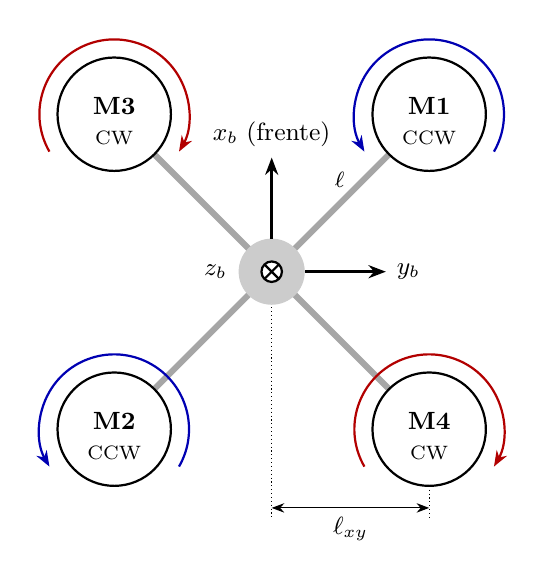
\begin{tikzpicture}[
    font=\small,
    seta/.style={-{Stealth[length=2.2mm]}},
    giro/.style={-{Stealth[length=2mm]}, thick},
    cota/.style={{Stealth[length=1.6mm]}-{Stealth[length=1.6mm]}},
]
    % braços
    \draw[line width=2.2pt, gray!70] (-2,-2) -- (2,2);
    \draw[line width=2.2pt, gray!70] (-2,2) -- (2,-2);
    \fill[gray!40] (0,0) circle (0.42);
    % rotores: posição na página (x = direita = y_b, y = cima = x_b)
    \foreach \x/\y/\n/\s in {2/2/1/CCW, -2/-2/2/CCW, -2/2/3/CW, 2/-2/4/CW} {
        \fill[white] (\x,\y) circle (0.72);
        \draw[thick] (\x,\y) circle (0.72);
        \node at (\x,\y+0.1) {\textbf{M\n}};
        \node[font=\scriptsize] at (\x,\y-0.3) {\s};
    }
    % sentido de giro visto de cima (anti-horário = CCW)
    \foreach \x/\y in {2/2, -2/-2}
        \draw[giro, blue!70!black] ($(\x,\y)+(-30:0.95)$)
            arc[start angle=-30, end angle=210, radius=0.95];
    \foreach \x/\y in {-2/2, 2/-2}
        \draw[giro, red!70!black] ($(\x,\y)+(210:0.95)$)
            arc[start angle=210, end angle=-30, radius=0.95];
    % eixos do corpo; z_b entra na página
    \draw[seta, very thick] (0,0.42) -- (0,1.45) node[above] {$x_b$ (frente)};
    \draw[seta, very thick] (0.42,0) -- (1.45,0) node[right] {$y_b$};
    \draw[thick, fill=white] (0,0) circle (0.13);
    \draw[thick] (-0.09,-0.09) -- (0.09,0.09) (-0.09,0.09) -- (0.09,-0.09);
    \node[left] at (-0.45,0) {$z_b$};
    % braço e alavanca
    \node[above left=-2pt, font=\footnotesize] at (1.0,1.0) {$\ell$};
    \draw[densely dotted] (0,-0.45) -- (0,-3.15);
    \draw[densely dotted] (2,-2.72) -- (2,-3.15);
    \draw[cota] (0,-3.0) -- (2,-3.0) node[midway, below] {$\ell_{xy}$};
\end{tikzpicture}
\fonte{Elaborada pelo autor.}
\end{figure}

A rolagem é produzida pela diferença de empuxo entre os lados direito e
esquerdo, e a arfagem, pela diferença entre a frente e a traseira. A guinada
não tem atuador próprio: resulta do desequilíbrio entre os torques de reação
dos pares que giram em sentidos opostos. Como esse torque de reação é muito
menor que o momento que o mesmo empuxo produz com o braço, a autoridade de
controle em guinada é muito inferior à de rolagem e arfagem --- característica
quantificada na Seção~\ref{sec:sitl} para a aeronave simulada.

\subsection{Hipóteses de modelagem}

O modelo é derivado sob as hipóteses usuais da
literatura~\cite{bouabdallah2007,beard2008,sabatino2015}:
\begin{alineas}
    \item a aeronave é um corpo rígido de massa constante, simétrico em relação
          aos planos $x_b z_b$ e $y_b z_b$, de modo que o tensor de inércia é
          diagonal, $\matriz{J} = \operatorname{diag}(J_{xx}, J_{yy}, J_{zz})$;
    \item o centro de massa coincide com a origem de $\{\mathcal{B}\}$ e está
          no plano dos rotores;
    \item o empuxo e o torque de reação de cada rotor são proporcionais ao
          quadrado da sua velocidade de rotação $\Omega_i$;
    \item a dinâmica dos motores e dos controladores eletrônicos de
          velocidade, o arrasto do corpo, o \textit{blade flapping} e o efeito
          solo são desprezados no modelo nominal e tratados como fontes
          conhecidas de discrepância.
\end{alineas}

\subsection{Equações de Newton-Euler}

A dinâmica de translação, escrita no referencial inercial, é
\begin{equation}
\dot{\vetor{p}} = \vetor{v}, \qquad
m\,\dot{\vetor{v}} = m g\,\vetor{e}_3 - T\,\matriz{R}\,\vetor{e}_3 + \vetor{f}_d,
\label{eq:translacao}
\end{equation}
em que $\vetor{p}$ e $\vetor{v}$ são a posição e a velocidade do centro de
massa, $\vetor{e}_3 = [0\ 0\ 1]^{\mathsf{T}}$, $T$ é o empuxo total, que atua
ao longo de $-z_b$, e $\vetor{f}_d$ reúne as forças de perturbação, entre elas
a força aerodinâmica devida ao vento. A dinâmica de rotação, escrita no
referencial do corpo, é dada pela equação de Euler~\cite{beard2008,beard2012}:
\begin{equation}
\matriz{J}\,\dot{\vetor{\omega}} =
-\vetor{\omega}\times\matriz{J}\,\vetor{\omega} + \vetor{\tau} + \vetor{\tau}_d,
\label{eq:rotacao-euler}
\end{equation}
em que $\vetor{\tau} = [\tau_x\ \tau_y\ \tau_z]^{\mathsf{T}}$ é o torque
produzido pelos rotores e $\vetor{\tau}_d$ é um torque de perturbação aditivo.
É por $\vetor{\tau}_d$ que entram, neste trabalho, os efeitos de momento não
modelados --- assimetrias, rajadas que atingem os rotores de forma desigual,
perda de eficiência de um rotor --- e as perturbações de torque usadas nos
ensaios (Seção~\ref{sec:perturbacoes}).

O conjunto formado por \eqref{eq:translacao}, \eqref{eq:rotacao-euler} e pela
cinemática \eqref{eq:cinematica-euler} ou \eqref{eq:cinematica-quaternio}
define um sistema de doze estados,
$\vetor{x} = [\vetor{p}^{\mathsf{T}}\ \vetor{v}^{\mathsf{T}}\
\phi\ \theta\ \psi\ \vetor{\omega}^{\mathsf{T}}]^{\mathsf{T}}$, com quatro
entradas, $\vetor{u} = [T\ \tau_x\ \tau_y\ \tau_z]^{\mathsf{T}}$. A
subatuação fica evidente: as acelerações horizontais não podem ser comandadas
diretamente, apenas por meio da inclinação do vetor de empuxo, o que impõe a
estrutura em cascata em que a atitude é a malha interna.

\subsection{Modelo dos rotores e matriz de alocação}

Cada rotor $i$ produz um empuxo $T_i = k_T\,\Omega_i^2$ ao longo de $-z_b$ e
um torque de reação $Q_i = k_Q\,\Omega_i^2 = \kappa\,T_i$ em torno de $z_b$,
com $\kappa = k_Q/k_T$. O torque de reação tem sentido oposto ao da rotação do
rotor: um rotor que gira no sentido anti-horário visto de cima (CCW) produz
sobre o corpo um torque no sentido horário, isto é, positivo em torno de
$z_b$. Com o motor $i$ na posição $(x_i, y_i)$ do plano dos rotores, o torque
do empuxo é $(x_i, y_i, 0)\times(0, 0, -T_i) = (-y_i T_i,\ x_i T_i,\ 0)$. Na
configuração X, $|x_i| = |y_i| = \ell_{xy} = \ell/\sqrt{2}$, e a numeração da
Figura~\ref{fig:quadx} leva à matriz de alocação
\begin{equation}
\begin{bmatrix} T \\ \tau_x \\ \tau_y \\ \tau_z \end{bmatrix} =
\underbrace{\begin{bmatrix}
1          & 1          & 1          & 1 \\
-\ell_{xy} & \ell_{xy}  & \ell_{xy}  & -\ell_{xy} \\
\ell_{xy}  & -\ell_{xy} & \ell_{xy}  & -\ell_{xy} \\
\kappa     & \kappa     & -\kappa    & -\kappa
\end{bmatrix}}_{\matriz{M}}
\begin{bmatrix} T_1 \\ T_2 \\ T_3 \\ T_4 \end{bmatrix}.
\label{eq:alocacao}
\end{equation}
A matriz $\matriz{M}$ é invertível, e $\matriz{M}^{-1}$ fornece os empuxos
individuais que realizam um par empuxo--torque desejado, desde que nenhum
deles saia da faixa disponível. A comparação entre a segunda e a quarta linhas
explica a fraca autoridade em guinada: um mesmo padrão de diferença de empuxo
produz torques na razão $\ell_{xy}/\kappa$ entre rolagem e guinada, da ordem
de 25 na aeronave simulada; como o torque de reação do SITL cresce com o
comando, a razão que vale para variações de empuxo é $\ell_{xy}/\kappa'$, com
$\kappa' = \mathrm{d}Q_i/\mathrm{d}T_i$, cerca de 15
(Seção~\ref{sec:forcas-momentos}).

% ----------------------------------------------------------------------
\section{Linearização em torno do voo pairado}
\label{sec:linearizacao}

O ponto de equilíbrio de interesse é o voo pairado: $\vetor{v} = \vetor{0}$,
$\phi = \theta = 0$, $\psi = \psi_0$, $\vetor{\omega} = \vetor{0}$, com
$T = mg$ e $\vetor{\tau} = \vetor{0}$. Tomando, sem perda de generalidade,
$\psi_0 = 0$ e desprezando produtos de pequenas variações, obtém-se de
\eqref{eq:rotacao}--\eqref{eq:rotacao-euler}
\begin{equation}
\delta\ddot{x} = -g\,\delta\theta, \quad
\delta\ddot{y} = g\,\delta\phi, \quad
\delta\ddot{z} = -\frac{\delta T}{m}, \quad
\ddot\phi = \frac{\tau_x}{J_{xx}}, \quad
\ddot\theta = \frac{\tau_y}{J_{yy}}, \quad
\ddot\psi = \frac{\tau_z}{J_{zz}}.
\label{eq:linear}
\end{equation}
O termo giroscópico $\vetor{\omega}\times\matriz{J}\vetor{\omega}$ e o
acoplamento da cinemática \eqref{eq:cinematica-euler} são de segunda ordem e
desaparecem; o sistema se decompõe em subsistemas de altitude, de atitude e de
posição horizontal, este último alimentado pela atitude. Essa estrutura
fundamenta tanto a arquitetura em cascata do firmware quanto o projeto do
controlador por eixo.

Cada eixo de atitude é, em primeira aproximação, um duplo
integrador~\cite{rao2001}. Para a
rolagem, com estado $\vetor{x}_\phi = [\phi\ \ p]^{\mathsf{T}}$,
\begin{equation}
\dot{\vetor{x}}_\phi =
\underbrace{\begin{bmatrix} 0 & 1 \\ 0 & 0 \end{bmatrix}}_{\matriz{A}}
\vetor{x}_\phi +
\underbrace{\begin{bmatrix} 0 \\ 1/J_{xx} \end{bmatrix}}_{\matriz{B}}
(\tau_x + \tau_{d,x}),
\qquad
\frac{\Phi(s)}{\tau_x(s)} = \frac{1}{J_{xx}\,s^2},
\label{eq:duplo-integrador}
\end{equation}
e analogamente para arfagem e guinada. O par $(\matriz{A}, \matriz{B})$ é
controlável, pois $[\matriz{B}\ \ \matriz{A}\matriz{B}]$ tem posto 2, e o par
$(\matriz{A}, \matriz{C})$ é observável já com
$\matriz{C} = [1\ \ 0]$~\cite{ogata2010}; na
prática, os dois estados são disponíveis, o ângulo pelo estimador e a
velocidade angular pelo giroscópio. Os dois autovalores na origem, num bloco
de Jordan, tornam o sistema instável em malha aberta. Em malha fechada, os
integradores da planta não ajudam a rejeitar um torque de perturbação
constante, porque ele entra antes deles: com realimentação proporcional dos
estados, $\tau_x = -J_{xx}\,(k_\theta\,\phi + k_\omega\,p)$, o ângulo se
acomoda num erro $\tau_{d,x}/(J_{xx}k_\theta)$. Erro nulo em regime exige um
integrador no controlador ou uma estimativa da perturbação, como prevê o
princípio do modelo interno~\cite{francis1976}.

Como o controlador é executado a cada $T_s$ segundos e o torque comandado é
mantido constante entre execuções, o modelo de projeto é a discretização por
segurador de ordem zero (ZOH)~\cite{franklin1998}:
\begin{equation}
\vetor{x}_{\phi,k+1} =
\begin{bmatrix} 1 & T_s \\ 0 & 1 \end{bmatrix} \vetor{x}_{\phi,k} +
\begin{bmatrix} T_s^2/(2J_{xx}) \\ T_s/J_{xx} \end{bmatrix} \tau_{x,k},
\label{eq:discreto}
\end{equation}
com $T_s = \SI{2.5}{\milli\second}$ para a taxa de \SI{400}{\hertz} usada
neste trabalho. O duplo integrador é o modelo \emph{nominal}; a planta efetiva
vista pelo controlador inclui ainda o filtro passa-baixas dos giroscópios, os
atrasos de amostragem e a saturação da alocação e, numa aeronave real, a
dinâmica dos motores, ausente no SITL (Seção~\ref{sec:motor-sitl}), que
acrescentam atraso de fase e limitam a banda passante alcançável. É essa
diferença que a identificação da Seção~\ref{sec:identificacao} quantifica.

% ----------------------------------------------------------------------
\section{Estimação e controle de atitude no ArduPilot}
\label{sec:ardupilot}

\subsection{Laço de execução}

No ArduCopter, a malha de atitude é executada no laço rápido do escalonador,
na taxa definida pelo parâmetro \codigo{SCHED\_LOOP\_RATE}, de
\SI{400}{\hertz} neste trabalho. A cada ciclo, na ordem definida em
\codigo{ArduCopter/Copter.cpp}~\cite{ardupilot2026}, o firmware lê os sensores
inerciais, executa o controlador de velocidade angular, executa o controlador
customizado, quando habilitado, envia os comandos aos motores e só então
atualiza o estimador de atitude e o modo de voo, cujo controlador de ângulo
produz o alvo de velocidade angular consumido no ciclo seguinte. A ordem
minimiza a latência entre a amostra do giroscópio e o comando dos motores. A
Figura~\ref{fig:cascata} resume a cadeia.

\begin{figure}[htbp]
\centering
\caption{Cadeia de controle de atitude do ArduCopter e ponto de inserção do
\codigo{AC\_CustomControl}. O modelador de referência fornece também a
velocidade angular de alimentação direta $\vetor{\omega}_{ff}$, e o
controlador customizado recebe as mesmas referências e estimativas que o
nativo.}
\label{fig:cascata}
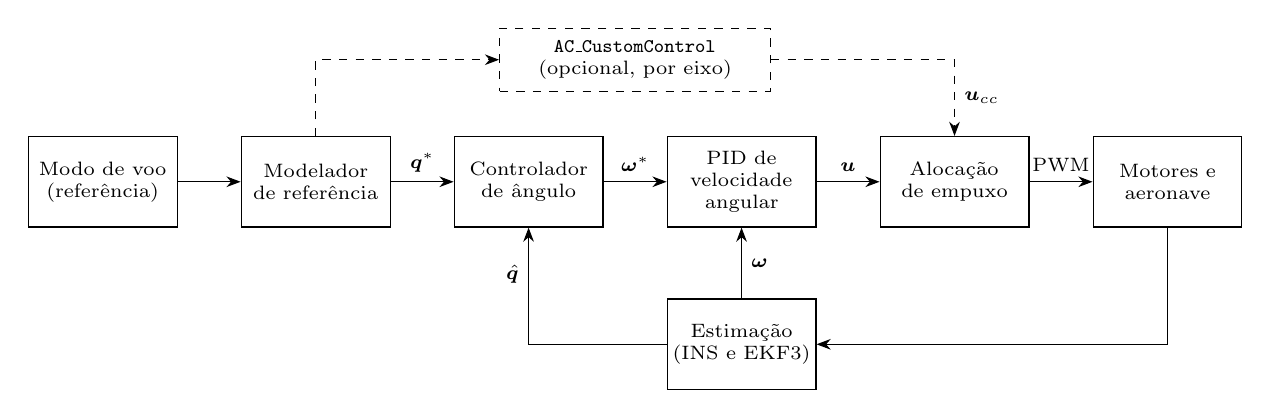
\begin{tikzpicture}[
    font=\scriptsize,
    bloco/.style={draw, rectangle, align=center, minimum height=1.15cm,
                  text width=1.75cm, inner sep=2pt},
    seta/.style={-{Stealth[length=1.8mm]}},
    node distance=0.8cm,
]
    \node[bloco] (ref) {Modo de voo\\(referência)};
    \node[bloco, right=of ref] (mod) {Modelador de referência};
    \node[bloco, right=of mod] (ang) {Controlador de ângulo};
    \node[bloco, right=of ang] (taxa) {PID de velocidade angular};
    \node[bloco, right=of taxa] (mix) {Alocação de empuxo};
    \node[bloco, right=of mix] (planta) {Motores e aeronave};
    \node[bloco, below=0.9cm of taxa] (est) {Estimação\\(INS e EKF3)};
    \node[bloco, dashed, text width=3.3cm, minimum height=0.8cm]
        (cc) at ($(ang)!0.5!(taxa) + (0,1.55)$)
        {\codigo{AC\_CustomControl}\\(opcional, por eixo)};

    \draw[seta] (ref) -- (mod);
    \draw[seta] (mod) -- node[above] {$\vetor{q}^*$} (ang);
    \draw[seta] (ang) -- node[above] {$\vetor{\omega}^*$} (taxa);
    \draw[seta] (taxa) -- node[above] {$\vetor{u}$} (mix);
    \draw[seta] (mix) -- node[above] {PWM} (planta);
    \draw[seta] (planta.south) |- (est.east);
    \draw[seta] (est.west) -| node[pos=0.8, left] {$\hat{\vetor{q}}$} (ang.south);
    \draw[seta] (est.north) -- node[right] {$\vetor{\omega}$} (taxa.south);
    \draw[seta, dashed] (mod.north) |- (cc.west);
    \draw[seta, dashed] (cc.east) -| node[pos=0.75, right] {$\vetor{u}_{cc}$} (mix.north);
\end{tikzpicture}
\fonte{Elaborada pelo autor com base em \citeonline{ardupilot2026}.}
\end{figure}

\subsection{Estimação de atitude}

Os sensores inerciais são integrados em incrementos de ângulo e de
velocidade. Como rotações finitas não comutam, a simples soma dos incrementos
do giroscópio acumula erro quando a aeronave oscila em mais de um eixo ao
mesmo tempo (efeito de \textit{coning}); o firmware aplica a correção de
\textit{coning} descrita por Tian et al.\ (2010, p.~26) \textit{apud}
\citeonline{ardupilot2026} antes de entregar os
incrementos ao estimador.

O estimador padrão é o EKF3, um filtro de Kalman estendido que funde os
sensores inerciais com GPS, barômetro e magnetômetro e estende o vetor de
estados com as polarizações dos sensores inerciais, o campo magnético e o
vento~\cite{ardupilotdev,ardupilot2026}. O EKF3 calcula ainda, por um filtro
complementar de terceira ordem baseado em \citeonline{widnall1980}, que
combina a aceleração vertical com a altura estimada, uma derivada da altura
cinematicamente consistente com ela; as malhas de altitude só a usam no lugar
da velocidade vertical do EKF quando esta não está disponível ou sob vibração
elevada. Como alternativa de contingência, o firmware mantém o
estimador \codigo{AP\_AHRS\_DCM}, um filtro complementar sobre a matriz de
cossenos diretores~\cite{premerlani2009}. Em todos os casos, a malha de
atitude recebe a atitude estimada $\hat{\vetor{q}}$ e a velocidade angular
$\vetor{\omega}$ medida pelo giroscópio após um filtro passa-baixas
(\SI{20}{\hertz} neste trabalho, parâmetro \codigo{INS\_GYRO\_FILTER}).

\subsection{Modelador de referência}

A referência que chega do modo de voo --- do piloto, no modo estabilizado, ou
das malhas externas, nos modos automáticos --- não é aplicada diretamente ao
controlador de ângulo. Ela passa por um modelador que gera uma atitude alvo
$\vetor{q}^*$ cinematicamente consistente, com aceleração angular limitada
pelos parâmetros \codigo{ATC\_ACC\_R\_MAX}, \codigo{ATC\_ACC\_P\_MAX} e
\codigo{ATC\_ACC\_Y\_MAX} e suavizada por uma constante de tempo
(\codigo{ATC\_INPUT\_TC} em rolagem e arfagem e \codigo{PILOT\_Y\_RATE\_TC}
em guinada). O modelador, habilitado por \codigo{ATC\_RATE\_FF\_ENAB} (padrão
1; com 0, a atitude alvo recebe a referência sem limitação de aceleração),
produz também a velocidade angular correspondente à trajetória do alvo,
$\vetor{\omega}_{ff}$, que é somada à saída do controlador de ângulo como
alimentação direta~\cite{ardupilot2026}. Um degrau
comandado ao firmware, portanto, não chega ao controlador como degrau, e sim
como uma transição de aceleração limitada; os ensaios deste trabalho medem a
resposta a essa referência modelada, que é a mesma para todos os
controladores.

\subsection{Controlador de ângulo}

O erro de atitude é calculado em quatérnio e decomposto em duas rotações
sucessivas: a que alinha o vetor de empuxo estimado ao alvo, que define os
erros de rolagem e arfagem, e a rotação residual em torno do eixo do empuxo,
que define o erro de guinada. A decomposição permite priorizar o vetor de
empuxo: quando o erro de inclinação supera \ang{30}, a correção de guinada é
atenuada, e o erro de guinada é limitado ao valor que saturaria a saída em
regime~\cite{ardupilot2026}.

Cada componente $e$ do erro é convertida em velocidade angular alvo por um
controlador proporcional com limite de aceleração, chamado no código de
controlador de raiz quadrada:
\begin{equation}
\omega^*(e) =
\begin{cases}
k\,e, & |e| \le e_{\mathrm{lin}}, \\[2pt]
\operatorname{sgn}(e)\sqrt{2\,a_{\max}\left(|e| - e_{\mathrm{lin}}/2\right)},
   & |e| > e_{\mathrm{lin}},
\end{cases}
\qquad e_{\mathrm{lin}} = \frac{a_{\max}}{k^2},
\label{eq:sqrt-controller}
\end{equation}
em que $k$ é o ganho \codigo{ATC\_ANG\_*\_P} e $a_{\max}$ é metade da
aceleração máxima do eixo, \codigo{ATC\_ACC\_*\_MAX}/2, limitada à faixa de
40 a \SI{720}{\degree\per\second\squared} em rolagem e arfagem e à de 10 a
\SI{120}{\degree\per\second\squared} em guinada. Para erros pequenos, a lei é linear; para erros
grandes, a velocidade angular cresce com a raiz do erro, o que garante que a
aeronave consiga desacelerar até o alvo sem exceder $a_{\max}$. As duas
expressões e suas derivadas coincidem em $|e| = e_{\mathrm{lin}}$. O resultado
é limitado às velocidades angulares máximas configuradas e somado à
alimentação direta $\vetor{\omega}_{ff}$, expressa no corpo, formando o alvo
$\vetor{\omega}^*$ do controlador de velocidade angular.

\subsection{Controlador de velocidade angular}

Cada eixo tem um controlador PID (\codigo{AC\_PID}) sobre o erro de
velocidade angular, cuja saída é um esforço normalizado em $[-1, 1]$, fração
do torque máximo disponível no eixo:
\begin{equation}
u = k_P\,e_f + \int_0^t k_I\,e_f\,\mathrm{d}t' + k_D\,\frac{\mathrm{d}e_f}{\mathrm{d}t}
    + k_{FF}\,\omega^*_f,
\qquad e_f = F_E\{\omega^*_f - \omega\},\quad \omega^*_f = F_T\{\omega^*\},
\label{eq:pid-taxa}
\end{equation}
em que $F_T$ e $F_E$ são filtros passa-baixas de primeira ordem sobre o alvo e
sobre o erro (\codigo{FLTT} e \codigo{FLTE}), e o termo derivativo tem o seu
próprio filtro (\codigo{FLTD}). O integrador é limitado a \codigo{IMAX} e,
quando a biblioteca de motores sinaliza saturação no eixo, só pode diminuir
em módulo, como proteção contra \textit{windup}~\cite[Cap.~10]{astrom2008}. A Tabela~\ref{tab:ganhos}
reúne os ganhos usados neste trabalho.

\begin{table}[htbp]
\centering
\caption{Ganhos do controlador de atitude nativo na linha de base
(\codigo{nativo.yaml}).}
\label{tab:ganhos}
\begin{tabular}{lccc}
\toprule
Parâmetro & Rolagem & Arfagem & Guinada \\
\midrule
Ganho de ângulo $k$ (\si{\per\second})      & 26,7     & 25,4     & 2,29 \\
$k_P$ de velocidade angular                 & 0,0862   & 0,0862   & 0,608 \\
$k_I$ de velocidade angular                 & 0,0862   & 0,0862   & 0,0608 \\
$k_D$ de velocidade angular                 & 0,000375 & 0,000375 & 0 \\
Limite do integrador (\codigo{IMAX})        & 0,5      & 0,5      & 0,5 \\
Filtro do alvo, \codigo{FLTT} (\si{\hertz}) & 20       & 20       & 20 \\
Filtro do erro, \codigo{FLTE} (\si{\hertz}) & ---      & ---      & 1 \\
Filtro do derivativo, \codigo{FLTD} (\si{\hertz}) & 20 & 20       & 20 \\
Aceleração máxima (\si{\degree\per\second\squared}) & 5857 & 5703 & 115 \\
\bottomrule
\end{tabular}


\fonte{\citeonline{ardupilot2026}; parâmetros gravados nos ensaios.}
\nota{\raggedright Ganhos, filtro do erro de guinada e acelerações máximas
obtidos pelo AutoTune do ArduPilot na própria aeronave simulada
(Seção~\ref{sec:autotune}); filtros do alvo e do derivativo e limite do
integrador, que o AutoTune não ajusta, nos padrões compilados. ``---'' indica
filtro desabilitado. As variantes \codigo{nativo\_lqi} e
\codigo{nativo\_filtro10} voam o mesmo controlador com outros ganhos
(Seção~\ref{sec:controladores}).}
\end{table}

\subsection{Alocação de empuxo}

Os esforços normalizados de rolagem, arfagem e guinada e o comando de empuxo
coletivo são combinados pela biblioteca \codigo{AP\_MotorsMatrix}, que
implementa uma versão normalizada de $\matriz{M}^{-1}$ em
\eqref{eq:alocacao}: cada motor recebe o empuxo coletivo somado aos esforços
ponderados por fatores de rolagem, arfagem e guinada próprios da sua posição e
do seu sentido de rotação. Quando a soma excede a faixa disponível, a
alocação dá prioridade à rolagem e à arfagem sobre a guinada, preservando
apenas uma folga mínima para a guinada (\codigo{MOT\_YAW\_HEADROOM}), e
sinaliza a saturação ao controlador. Por fim, o empuxo desejado $t \in [0,1]$
de cada motor é convertido em comando $c$ pela inversa da curva de empuxo
$t = (1-e)\,c + e\,c^2$:
\begin{equation}
c = \frac{-(1-e) + \sqrt{(1-e)^2 + 4\,e\,t}}{2\,e},
\label{eq:linearizacao-empuxo}
\end{equation}
com $e$ dado por \codigo{MOT\_THST\_EXPO}, de modo que o esforço do controlador
seja aproximadamente linear em empuxo; o comando é então mapeado na faixa útil
do motor e convertido em largura de pulso.

\subsection{O \textit{framework} \texorpdfstring{\codigo{AC\_CustomControl}}{AC\_CustomControl}}
\label{sec:customcontrol}

O \codigo{AC\_CustomControl} é a biblioteca do ArduPilot destinada a
hospedar controladores de atitude alternativos sem alterar o restante do
firmware~\cite{ardupilot2026}. Sua função de atualização é chamada no laço
rápido logo depois do controlador de velocidade angular nativo e antes da
saída para os motores (Figura~\ref{fig:cascata}); ela recebe a mesma atitude
alvo, a mesma alimentação direta e as mesmas estimativas usadas pelo
controlador nativo e devolve os esforços de rolagem, arfagem e guinada,
que sobrescrevem os do nativo antes da alocação. A latência adicional é,
portanto, nula.

O \textit{framework} separa uma interface comum (\textit{frontend}) das
implementações (\textit{backends}). O parâmetro \codigo{CC\_TYPE} escolhe o
\textit{backend} --- 1 para um modelo vazio e 2 para um PID de exemplo, com
parâmetros próprios de prefixo \codigo{CC2\_} --- e \codigo{CC\_AXIS\_MASK}
escolhe, por máscara de bits, em quais eixos a saída do controlador
customizado substitui a do nativo. A ativação em voo é feita por uma chave do
rádio configurada com a função 109. Na volta ao controlador nativo, o
\textit{framework} zera os integradores do PID nativo e, com
\codigo{ATC\_RATE\_FF\_ENAB} habilitado, leva a atitude alvo e o alvo de
velocidade angular ao estado atual da aeronave e reinicializa os filtros dos
PIDs, para suavizar a transição; enquanto o \textit{backend} está ativo, os
integradores do nativo são zerados a cada laço nos eixos que ele controla. O
\textit{backend} de exemplo reproduz a arquitetura nativa de ângulo e
velocidade angular sem as suas proteções: o controlador de ângulo é só
proporcional, sem o controlador de raiz quadrada e sem a atenuação da guinada
acima de \ang{30}, e o PID de velocidade angular não recebe o sinal de
saturação da alocação. Os ganhos padrão são 90\,\% dos padrões compilados do
nativo; por isso serve como verificação do procedimento de ensaio, e não como
controlador alternativo. Os controladores propostos neste trabalho são
implementados como dois novos
\textit{backends} (Capítulo~\ref{cap:projeto}).

% ----------------------------------------------------------------------
\section{Técnicas de controle}
\label{sec:tecnicas}

\subsection{Controle PID em tempo discreto}

O controlador PID combina uma ação proporcional ao erro, uma ação integral,
que elimina o erro em regime diante de perturbações constantes, e uma ação
derivativa, que antecipa a tendência do erro~\cite{astrom2008,ogata2010}. Na
implementação digital, três cuidados são essenciais: a derivada deve ser
filtrada, porque a diferenciação amplifica o ruído de medição; o integrador
deve ser protegido contra \textit{windup} quando o atuador satura; e a
discretização deve preservar o comportamento contínuo na faixa de frequências
de interesse, o que exige taxa de amostragem bem acima da banda passante da
malha~\cite{franklin1998,wang2020}. A Equação~\eqref{eq:pid-taxa} mostra como o
ArduPilot trata esses três pontos, e acrescenta um termo de alimentação
direta que reduz a carga sobre a realimentação no rastreamento.

\subsection{Realimentação de estados e regulador linear quadrático}

Na realimentação de estados, a lei de controle $\vetor{u} = -\matriz{K}\vetor{x}$
aloca os autovalores de malha fechada $\matriz{A} - \matriz{B}\matriz{K}$
sempre que o par $(\matriz{A}, \matriz{B})$ é
controlável~\cite{ogata2010,fadali2009}.
No regulador linear quadrático (LQR), em vez de especificar os autovalores, o
projetista especifica o compromisso entre desvio dos estados e esforço de
controle por meio do custo
\begin{equation}
\mathcal{J} = \sum_{k=0}^{\infty}
\left(\vetor{x}_k^{\mathsf{T}}\matriz{Q}\,\vetor{x}_k
    + \vetor{u}_k^{\mathsf{T}}\matriz{R}_u\,\vetor{u}_k\right),
\qquad \matriz{Q} \succeq 0,\ \matriz{R}_u \succ 0,
\label{eq:custo-lqr}
\end{equation}
cujo mínimo, para o sistema discreto
$\vetor{x}_{k+1} = \matriz{A}_d\vetor{x}_k + \matriz{B}_d\vetor{u}_k$, é
atingido pelo ganho~\cite{franklin1998,datta2003}
\begin{equation}
\matriz{K} = \left(\matriz{R}_u + \matriz{B}_d^{\mathsf{T}}\matriz{P}\matriz{B}_d\right)^{-1}
             \matriz{B}_d^{\mathsf{T}}\matriz{P}\matriz{A}_d,
\label{eq:ganho-lqr}
\end{equation}
em que $\matriz{P}$ é a solução estabilizante, simétrica e semidefinida
positiva, da equação algébrica de Riccati discreta
\begin{equation}
\matriz{P} = \matriz{A}_d^{\mathsf{T}}\matriz{P}\matriz{A}_d
 - \matriz{A}_d^{\mathsf{T}}\matriz{P}\matriz{B}_d
   \left(\matriz{R}_u + \matriz{B}_d^{\mathsf{T}}\matriz{P}\matriz{B}_d\right)^{-1}
   \matriz{B}_d^{\mathsf{T}}\matriz{P}\matriz{A}_d + \matriz{Q}.
\label{eq:riccati}
\end{equation}
Essa solução existe e é única quando o par $(\matriz{A}_d, \matriz{B}_d)$ é
estabilizável e o par $(\matriz{A}_d, \matriz{Q}^{1/2})$ é
detectável~\cite{datta2003}; nos eixos deste trabalho, as duas condições
valem, porque a planta é controlável e $\matriz{Q}$ é diagonal positiva. Uma
escolha inicial usual para as ponderações é normalizar cada estado e cada
entrada pelo seu valor máximo admissível (regra de Bryson; ver
\citeonline{hespanha2009}), refinando-as a seguir pela resposta
de malha fechada. Com realimentação de todos os estados, o LQR de tempo
contínuo tem margens de estabilidade garantidas em cada canal de entrada:
tolera aumento ilimitado ou redução de até 50\,\% do ganho e tem margem de
fase de ao menos \ang{60}~\cite{safonov1977}. Em tempo discreto, mesmo com
realimentação de todos os estados, as margens garantidas são menores e
dependem de $\matriz{R}_u$ e de $\matriz{B}_d^{\mathsf{T}}\matriz{P}\matriz{B}_d$~\cite{shaked1986};
com estimador, deixam de existir~\cite{doyle1978}; e os filtros e atrasos da
planta real as reduzem ainda mais. Por isso as margens são verificadas em
cada projeto.

A realimentação de estados pura não anula o erro em regime diante de uma
perturbação constante, que é o caso de $\vetor{\tau}_d$ em degrau. A solução
clássica~\cite{young1972} é aumentar o vetor de estados com a integral do erro de
rastreamento, $x_{I,k+1} = x_{I,k} + T_s\,(r_k - y_k)$, e projetar o LQR sobre
o sistema aumentado, chamado LQI (\textit{linear quadratic integral}), o que
preserva a formulação de projeto ao custo de um
estado a mais por eixo e da necessidade de proteção contra \textit{windup}.

\subsection{Observador de estado estendido}

Uma alternativa à ação integral é estimar a perturbação e cancelá-la. No
controle por rejeição ativa de perturbações (ADRC), sistematizado em inglês
por \citeonline{han2009}, todo o efeito que separa a planta de um modelo nominal
simples --- perturbações externas, erros de modelo e acoplamentos --- é
agrupado em uma \emph{perturbação total} $f$, tratada como estado adicional e
estimada por um observador de estado estendido (ESO). Para um eixo de atitude
com a velocidade angular medida, a dinâmica se escreve
$\dot p = b_0\,u + f$, com $b_0$ a estimativa do ganho de controle, e um ESO
linear de segunda ordem é~\cite{gao2003}
\begin{equation}
\dot{\hat p} = \hat f + b_0\,u + l_1\,(p - \hat p), \qquad
\dot{\hat f} = l_2\,(p - \hat p),
\label{eq:eso}
\end{equation}
com $l_1$ e $l_2$ escolhidos para alocar os polos do observador. A lei de
controle $u = (u_0 - \hat f)/b_0$ reduz o eixo, dentro da banda do observador,
ao duplo integrador nominal, sobre o qual $u_0$ é projetado. O compromisso
central está na banda do observador: quanto maior, mais rápida a estimativa da
perturbação e maior a sensibilidade ao ruído do giroscópio.

\subsection{Filtro de Kalman e controle LQG}
\label{sec:lqg}

A lei $\vetor{u} = -\matriz{K}\vetor{x}$ supõe todos os estados medidos sem
erro. Quando parte deles não é medida, ou é medida com ruído e por um caminho
com dinâmica própria, o estado é estimado a partir de um modelo. Seja o
sistema discreto
\begin{equation}
\vetor{x}_{k+1} = \matriz{A}_d\vetor{x}_k + \matriz{B}_d\vetor{u}_k
                + \matriz{G}\,\vetor{w}_k,
\qquad
\vetor{y}_k = \matriz{C}\vetor{x}_k + \vetor{v}_k,
\label{eq:modelo-estocastico}
\end{equation}
com $\vetor{w}_k$ e $\vetor{v}_k$ ruídos brancos independentes, de
covariâncias $\matriz{W}$ e $\matriz{V}$. O filtro de
Kalman~\cite{kalman1960b} corrige a predição do modelo pela inovação, a
diferença entre a medida e a sua predição:
\begin{equation}
\hat{\vetor{x}}_{k|k} = \hat{\vetor{x}}_{k|k-1}
    + \matriz{L}\left(\vetor{y}_k - \matriz{C}\,\hat{\vetor{x}}_{k|k-1}\right),
\qquad
\hat{\vetor{x}}_{k+1|k} = \matriz{A}_d\hat{\vetor{x}}_{k|k} + \matriz{B}_d\vetor{u}_k.
\label{eq:kalman}
\end{equation}
Em regime, o ganho $\matriz{L}$ é constante e sai de uma equação de Riccati
com a forma de~\eqref{eq:riccati}, com $\matriz{A}_d^{\mathsf{T}}$ e
$\matriz{C}^{\mathsf{T}}$ no lugar de $\matriz{A}_d$ e $\matriz{B}_d$ e com as
covariâncias $\matriz{G}\matriz{W}\matriz{G}^{\mathsf{T}}$ e $\matriz{V}$ no
lugar das ponderações: é a dualidade entre o filtro e o
regulador~\cite{kalman1960b}. Como no ESO, o vetor de estados pode ser
estendido com a perturbação, modelada como passeio aleatório, que o filtro
passa a estimar; e pode ser estendido também com a dinâmica do caminho de
medida --- filtros, atrasos e polarizações dos sensores ---, que o ESO
de~\eqref{eq:eso} ignora. É o que faz o controlador LQG deste trabalho
(Capítulo~\ref{cap:projeto}).

O controlador LQG (\textit{linear quadratic Gaussian}) aplica o ganho do LQR
ao estado estimado, $\vetor{u}_k = -\matriz{K}\hat{\vetor{x}}_{k|k}$, e trata
o projeto como um problema estocástico de regulação~\cite{athans1971}. Pelo
princípio da separação~\cite{joseph1961}~\cite[seção~8.2]{anderson1989}, os
autovalores da malha fechada são a união dos autovalores da realimentação de
estados, $\matriz{A}_d - \matriz{B}_d\matriz{K}$, com os do erro de
estimação, e $\matriz{K}$ e $\matriz{L}$ podem ser projetados separadamente.
A separação vale para a estabilidade nominal, mas não para a robustez: as
margens garantidas do LQR com realimentação de todos os estados não se
transferem ao LQG, cujas margens dependem do projeto e precisam ser
verificadas~\cite{doyle1978}. Uma forma de recuperá-las é a recuperação da
malha (LTR, \textit{loop transfer recovery}): aumentando a intensidade do
ruído fictício de processo na entrada da planta, a função de transferência de
malha na entrada da planta tende à do LQR com realimentação de todos os
estados~\cite{doyle1979,doyle1981}~\cite[seção~8.4]{anderson1989}. A
recuperação exige planta de fase mínima e, em tempo discreto e com atraso na
medida, pode ser incompleta; o seu preço é um estimador mais rápido, que deixa
passar mais ruído de medida para o esforço de controle
(Capítulo~\ref{cap:projeto}).

\subsection{Limite de desempenho: a integral de Bode}
\label{sec:bode}

Seja $L(z)$ o ganho de malha aberta de um eixo, que inclui o controlador e a
planta $P(z)$, e $S(z) = 1/[1 + L(z)]$ a função de sensibilidade. Um torque
de perturbação que entra na planta chega ao ângulo por $P(z)\,S(z)$, a
sensibilidade à perturbação na entrada da planta~\cite{landau2011}, e não por
$S(z)$: é essa a grandeza que as varreduras de torque deste trabalho estimam
(Seção~\ref{sec:identificacao}). Para $L(z)$ estritamente própria e sem polos
fora do círculo unitário, como nos eixos deste trabalho, a sensibilidade em
tempo discreto obedece a~\cite{sung1988,mohtadi1990}
\begin{equation}
\frac{1}{\pi}\int_0^{\pi}\ln\left|S\!\left(\mathrm{e}^{\mathrm{j}\vartheta}\right)\right|
\mathrm{d}\vartheta = 0,
\qquad \vartheta = \omega\,T_s,
\label{eq:bode}
\end{equation}
versão discreta da integral de sensibilidade de
\citeonline{bode1945}; com polos instáveis em malha aberta, o lado direito
passa a ser positivo~\cite{freudenberg1985}. A atenuação da perturbação numa
faixa de frequências ($|S| < 1$) é paga com amplificação em outra
($|S| > 1$), em áreas iguais de $\ln|S|$: é o efeito conhecido como colchão
d'água, que nenhuma lei de controle linear e invariante no tempo contorna;
\citeonline{iglesias2001} estende a restrição a sistemas lineares variantes no
tempo. Em tempo discreto, a integral cobre uma faixa finita, de 0 à
frequência de Nyquist, e a amplificação não pode ser diluída numa banda
arbitrariamente larga, como no caso contínuo; com o laço a \SI{400}{\hertz}
e o filtro de \SI{20}{\hertz}, o compromisso fica mais apertado.
Como a planta $P$ é a mesma para todos os controladores, a diferença entre os
$\ln|P\,S|$ medidos com dois controladores é a diferença entre os seus
$\ln|S|$, e a comparação das varreduras de torque herda a
restrição~\eqref{eq:bode}.

% ----------------------------------------------------------------------
\section{Modelos de perturbação}
\label{sec:perturbacoes}

\subsection{Perturbações de torque}

Um vento uniforme aplicado ao centro de massa produz força, mas não momento:
afeta a posição e, apenas indiretamente, a atitude. Em uma aeronave real, o
vento também gera momentos --- pelo afastamento entre o centro de pressão e o
centro de massa, pelo \textit{blade flapping} e pela incidência desigual nos
rotores --- e são esses momentos que exercitam a malha de atitude. Para
avaliar a malha de atitude de forma direta e controlada, empregam-se
perturbações aditivas de torque, isto é, o termo $\vetor{\tau}_d$ de
\eqref{eq:rotacao-euler}, em quatro formas: o \emph{pulso retangular}, cujo
impulso angular é conhecido de antemão e que mede a recuperação após um
deslocamento; o \emph{degrau sustentado}, que expõe o erro em regime e a
suficiência da ação integral; a \emph{varredura em frequência}, que
caracteriza, ao longo de uma faixa de frequências, a resposta do ângulo ao
torque de perturbação, isto é, a sensibilidade à perturbação na entrada da
planta (Seção~\ref{sec:bode}); e o \emph{torque estocástico}, um processo de
Gauss-Markov de primeira ordem em cada eixo --- o processo de
Ornstein-Uhlenbeck~\cite{uhlenbeck1930} ---, que representa uma perturbação
contínua de banda limitada e é avaliado pelo erro quadrático médio. Com
desvio-padrão $\sigma$ e tempo de correlação $\tau$, o processo admite
discretização exata~\cite{gillespie1996}:
\begin{equation}
x_{k+1} = \mathrm{e}^{-\Delta t/\tau}\,x_k
        + \sigma\sqrt{1 - \mathrm{e}^{-2\Delta t/\tau}}\;w_k,
\qquad w_k \sim \mathcal{N}(0,1),
\label{eq:gauss-markov-discreto}
\end{equation}
que preserva a variância $\sigma^2$ para qualquer passo $\Delta t$.

Para que os ensaios sejam reprodutíveis, o ruído branco $w_k$ deve ser gerado
de forma determinística a partir de uma semente. Neste trabalho, ele é
obtido de um gerador congruencial linear multiplicativo,
$x_{k+1} = 16807\,x_k \bmod (2^{31}-1)$, o padrão mínimo de
\citeonline{park1988}, calculado sem estouro em aritmética de 32 bits pelo
método de \citeonline{schrage1979}, cujas amostras uniformes são convertidas em amostras
gaussianas pela transformação de \citeonline{box1958}. A mesma transformação,
na variante polar de \citeonline{marsaglia1964}, que dispensa seno e cosseno,
é a que o SITL usa (\codigo{Aircraft::rand\_normal}) na turbulência nativa do
vento e no ruído dos sensores do modelo de avião; no multirrotor, o ruído dos
sensores inerciais simulados é uniforme.

\subsection{Vento}

O vento que atua sobre a aeronave é usualmente decomposto em uma parcela
constante e uma parcela de rajadas, modelada como processo
estocástico~\cite{beard2012}. No SITL, o vento uniforme age quase só sobre a
posição (Seção~\ref{sec:sitl}), e nenhum ensaio de atitude deste trabalho
depende dele. Os modelos de vento do injetor --- o vento médio, a rajada
discreta da norma MIL-F-8785C~\cite{mil8785c} e a turbulência de Dryden, com
a sua discretização --- estão no Apêndice~\ref{ap:vento}.

% ----------------------------------------------------------------------
\section{Identificação de sistemas no domínio da frequência}
\label{sec:identificacao}

A identificação no domínio da frequência estima a resposta em frequência de
um sistema a partir de registros de entrada e saída obtidos sob uma excitação
de banda larga~\cite{ljung1999,pintelon2012,tischler2012}. A excitação mais usada em
aeronaves é a varredura senoidal de frequência crescente (\textit{chirp}). O
modo \textit{System Identification} do ArduCopter (modo 25) gera uma
varredura exponencial, implementada em
\codigo{AP\_Math/chirp.cpp}~\cite{ardupilot2026}, cuja frequência instantânea
é
\begin{equation}
\omega(t) = \omega_{\min}\,\exp\!\left(B\,\frac{t - t_c}{T_r - t_c}\right),
\qquad B = \ln\frac{\omega_{\max}}{\omega_{\min}},
\label{eq:chirp}
\end{equation}
precedida por um intervalo de duração $t_c$ em frequência constante
$\omega_{\min}$ e modulada por janelas de cosseno no início e no fim do
registro de duração $T_r$, de modo que a excitação comece e termine suave.
A varredura exponencial dedica o mesmo tempo a cada década, o que favorece as
baixas frequências.

A resposta em frequência é estimada pela razão entre a densidade espectral
cruzada da entrada $u$ com a saída $y$ e a densidade espectral da
entrada~\cite{carter1973,tischler2012},
\begin{equation}
\hat H(f) = \frac{\hat G_{uy}(f)}{\hat G_{uu}(f)},
\qquad
\hat\gamma^2_{uy}(f) = \frac{|\hat G_{uy}(f)|^2}{\hat G_{uu}(f)\,\hat G_{yy}(f)},
\label{eq:frf}
\end{equation}
com as densidades estimadas pelo método de \citeonline{welch1967}, que divide
o registro em segmentos sobrepostos, aplica uma janela a cada um e faz a
média dos periodogramas, trocando resolução em frequência por menor
variância. A coerência $\hat\gamma^2_{uy} \in [0, 1]$ mede a fração da saída
linearmente explicada pela entrada: valores baixos indicam ruído,
não linearidade ou excitação insuficiente naquela frequência, e
\citeonline{tischler2012} recomendam usar apenas os pontos de coerência
elevada (da ordem de 0,6 ou mais) no ajuste de modelos paramétricos. O ajuste
de uma função de transferência a $\hat H(f)$ por mínimos quadrados fornece o
modelo identificado, comparado ao modelo analítico
\eqref{eq:duplo-integrador}~\cite{ljung1999,pintelon2012}.

% ----------------------------------------------------------------------
\section{Simulação \textit{software-in-the-loop}}
\label{sec:sitl}

No SITL do ArduPilot, o próprio código do firmware é compilado para o
computador de desenvolvimento, com uma camada de abstração de
\textit{hardware} (HAL) que substitui os sensores e os atuadores por um modelo
físico do veículo~\cite{ardupilotdev}. O código de estimação e de controle é
o mesmo que roda na controladora de voo; o que muda é a origem das medidas e
o destino dos comandos de PWM. O relógio é simulado e avança junto com o
modelo físico, de modo que os resultados não dependem da carga do computador,
e a comunicação com o veículo usa o protocolo MAVLink, como em um voo real.

\subsection{Modelo de multirrotor}

O modelo físico de multirrotor do SITL, implementado em
\codigo{SIM\_Frame.cpp} e \codigo{SIM\_Motor.cpp}, na pasta
\codigo{libraries/SITL} do firmware, calcula, a cada passo, o empuxo e o
torque de cada motor a partir do seu comando $c \in [0, 1]$:
\begin{equation}
T_i = T_{\max}\left[(1-e)\,c_i + e\,c_i^2\right], \qquad
Q_i = 0{,}05\,D\,T_i\,c_i,
\label{eq:motor-sitl}
\end{equation}
em que $e$ é o expoente da curva de empuxo e $D$ é o parâmetro de tamanho do
quadro; a variação dos comandos é limitada em taxa. O torque de reação cresce,
portanto, com o comando, e a razão $\kappa = Q_i/T_i$ de
\eqref{eq:alocacao} vale $0{,}05\,D\,c$. Quando o tensor de inércia não é
informado, o simulador o estima supondo metade da massa distribuída em um anel
de raio $D/2$:
$J_{xx} = J_{yy} = m\,(D/2)^2/4$ e $J_{zz} = m\,(D/2)^2/2$.

A dinâmica de rotação é integrada no referencial do corpo como
\begin{equation}
\dot{\vetor{\omega}} = \matriz{J}^{-1}\left(\vetor{\tau} + \vetor{\tau}_{md}\right)
                     - a_r\,\vetor{\omega} + \vetor{a}_{\mathrm{tw}},
\label{eq:rotacao-sitl}
\end{equation}
em que $\vetor{\tau}_{md}$ é o torque do arrasto de momento dos rotores ---
cada rotor, ao se deslocar com a rotação do corpo, sofre uma força contrária à
sua velocidade ---, $a_r$ é um amortecimento rotacional linear explícito, de
constante de tempo da ordem de \SI{17}{\second}, e
$\vetor{a}_{\mathrm{tw}}$ é uma aceleração angular aditiva, ajustável pelos
parâmetros \codigo{SIM\_TWIST\_*}, que realiza exatamente o termo
$\matriz{J}^{-1}\vetor{\tau}_d$ de \eqref{eq:rotacao-euler}. É o arrasto de
momento que domina o amortecimento: com ele, a constante de tempo da
velocidade angular cai para cerca de \SI{0.5}{\second}
(Seção~\ref{sec:movimento}), ainda lenta perto da banda do controle. O termo
giroscópico $\vetor{\omega}\times\matriz{J}\vetor{\omega}$ \emph{não} é
modelado. Para uma aeronave com $J_{xx} = J_{yy}$, ele só afetaria rolagem e
arfagem, por meio do produto de duas velocidades angulares, e é desprezível
perto do pairado; a consequência é que a planta simulada está mais próxima do
modelo linear \eqref{eq:duplo-integrador} do que uma aeronave real estaria. O
vento (\codigo{SIM\_WIND\_*}) entra no modelo pela velocidade relativa do ar,
por dois caminhos: o arrasto de corpo, aplicado no centro de massa e sem
momento, e o arrasto de momento de cada rotor, aplicado na posição do rotor e
proporcional à raiz do seu empuxo. Com empuxos iguais, os momentos deste
último se cancelam, e com empuxos diferentes sobra um momento pequeno: o vento
move a aeronave, mas praticamente não perturba a atitude. Essa é a razão pela
qual os ensaios de rejeição de perturbação na malha de atitude usam
perturbações de torque.

\subsection{Sensores inerciais simulados}
\label{sec:sensores-sitl}

Com \codigo{INS\_FAST\_SAMPLE} ligado, como nos ensaios, o giroscópio
simulado é amostrado oito vezes por leitura, e a leitura entregue ao firmware
é a média das oito sub-amostras (\codigo{AP\_InertialSensor\_SITL.cpp}). A
cada sub-amostra, o SITL soma à velocidade angular verdadeira um ruído
uniforme de $\pm\SI{0.04}{\degree\per\second}$, sempre presente, e, com os
motores ligados, um segundo ruído uniforme, de amplitude igual a
\codigo{SIM\_GYR1\_RND} vezes o acelerador. Com a média, um ruído uniforme de
amplitude $A$ por sub-amostra chega ao firmware com desvio-padrão
$A/\sqrt{3 \cdot 8}$: o ruído mínimo fica da ordem de
\SI{0.01}{\degree\per\second}, e o giroscópio dos ensaios com
\codigo{SIM\_GYR1\_RND} nulo é, assim, praticamente sem ruído. Há ainda uma
deriva lenta, de \SI{0.05}{\degree\per\second} por minuto
(\codigo{SIM\_DRIFT\_SPEED}), que o EKF3 estima como polarização.

O filtro passa-baixas de \SI{20}{\hertz} (\codigo{INS\_GYRO\_FILTER}) só se
aplica à velocidade angular entregue aos controladores. Os incrementos de
ângulo que alimentam o estimador de atitude são integrados do giroscópio
antes do filtro (\codigo{AP\_InertialSensor\_Backend.cpp}): em horizontes
curtos, o ângulo estimado acompanha a integral do giroscópio sem o atraso do
filtro, mas com o ruído integrado, e chega ao controlador com um laço de
atraso (Seção~\ref{sec:instrumentacao}). O ruído, a média das sub-amostras e
o ângulo calculado sem o filtro definem o caminho de medida que o estimador do
controlador LQG modela (Capítulo~\ref{cap:projeto}).

\subsection{Aeronave simulada}

Os ensaios usam o modelo de quadrirrotor X padrão do SITL, cujos parâmetros
estão na Tabela~\ref{tab:aeronave}. Com eles, a alavanca de rolagem e arfagem
é $\ell_{xy} = \SI{0.247}{\metre}$, enquanto a razão entre torque de reação e
empuxo no pairado é $\kappa = \SI{0.0096}{\metre}$, nas condições de
referência do modelo. Como o torque de reação
cresce com o comando, a razão que vale para \emph{variações} de empuxo é
maior, cerca de \SI{0.0165}{\metre} (Seção~\ref{sec:motor-sitl}); ainda
assim, um mesmo padrão de diferença de empuxo produz um torque de guinada
cerca de 15 vezes menor que o de rolagem e, como $J_{zz} = 2J_{xx}$, uma
aceleração angular cerca de 30 vezes menor. A assimetria reaparece nas
acelerações máximas que o AutoTune registrou para o modelador de referência:
\SI{115}{\degree\per\second\squared} em guinada, contra cerca de
\SI{5800}{\degree\per\second\squared} em rolagem e arfagem
(Tabela~\ref{tab:ganhos}). A razão, de 50, não coincide com a de autoridade,
porque o AutoTune grava a aceleração atingida nos seus ensaios de ângulo, que
depende também dos ganhos, e não a máxima disponível.

\begin{table}[htbp]
\centering
\caption{Parâmetros do quadrirrotor X simulado.}
\label{tab:aeronave}
\begin{tabular}{lll}
\toprule
Grandeza & Valor & Origem \\
\midrule
Massa $m$                                   & \SI{3.0}{\kilogram} & \codigo{SIM\_FRM\_MASS} \\
Braço $\ell$ (centro ao motor)              & \SI{0.35}{\metre}   & \codigo{SIM\_FRM\_DIAG\_SZ}\textsuperscript{(a)} \\
Alavanca de rolagem e arfagem $\ell_{xy}$   & \SI{0.247}{\metre}  & $\ell/\sqrt{2}$ \\
Inércia $J_{xx} = J_{yy}$                   & \SI{0.02297}{\kilogram\metre\squared} & estimada pelo SITL \\
Inércia $J_{zz}$                            & \SI{0.04594}{\kilogram\metre\squared} & estimada pelo SITL \\
Empuxo máximo por motor $T_{\max}$          & \SI{18.86}{\newton} & calculado pelo SITL \\
Empuxo por motor no pairado                 & \SI{7.35}{\newton}, com $c = 0{,}551$ & $mg/4$ \\
Razão empuxo/peso                           & 2,56 & --- \\
Expoente da curva de empuxo $e$             & 0,65 & \codigo{SIM\_FRM\_EXPO} \\
Razão $\kappa$ no pairado                   & \SI{0.0096}{\metre} & $0{,}05\,D\,c$ \\
Taxa do modelo físico                       & \SI{1200}{\hertz} & \codigo{SIM\_RATE\_HZ} \\
Taxa do laço de controle                    & \SI{400}{\hertz} & \codigo{SCHED\_LOOP\_RATE} \\
\bottomrule
\end{tabular}


\fonte{Parâmetros gravados nos ensaios e código-fonte do SITL
\cite{ardupilot2026}.}
\nota{\raggedright (a) Apesar do nome (``diagonal''), o SITL posiciona cada motor a essa
distância do \emph{centro}; a distância entre motores opostos é, por isso,
\SI{0.70}{\metre}.}
\end{table}

% Próximos capítulos (ver Seção "Organização do trabalho").
% ======================================================================
%  CAPÍTULO 3 — MATERIAIS E MÉTODOS
%
%  Descreve o que está implementado em ensaios/: o ambiente (SITL puro), o
%  injetor de perturbações (lua/vento.lua), os controladores e o AutoTune
%  (controladores/, autotune.py), os cenários (cenarios/<eixo>/), as métricas
%  (analise/metricas.py, analise/frequencia.py) e a automação
%  (run_ensaio.py). Os números de procedimento vêm do código e do README.
% ======================================================================
\chapter{Materiais e métodos}
\label{cap:metodos}

Este capítulo descreve o ambiente em que os controladores são ensaiados e o
procedimento que transforma um ensaio em números comparáveis. O princípio que
orienta todas as escolhas é o de que dois controladores só podem ser
comparados se enfrentarem exatamente as mesmas condições: a mesma aeronave, a
mesma perturbação, no mesmo instante, com o mesmo estado inicial, e medidos
pelas mesmas métricas, calculadas na mesma janela. Por isso o procedimento é
inteiramente automatizado, e cada ensaio deixa registrado tudo o que é
necessário para auditá-lo depois.

% ----------------------------------------------------------------------
\section{Ambiente de simulação}
\label{sec:ambiente}

Os ensaios usam o firmware ArduCopter na versão de desenvolvimento 4.8,
fixado no \textit{commit} \codigo{ce9c2d01a4} do repositório
oficial~\cite{ardupilot2026}, executado em SITL com o modelo de multirrotor
nativo do simulador (Seção~\ref{sec:sitl}), na configuração X
(\codigo{FRAME\_CLASS} = 1, \codigo{FRAME\_TYPE} = 1). O modelo físico é
integrado a \SI{1200}{\hertz} e o laço de controle roda a \SI{400}{\hertz}
(Tabela~\ref{tab:aeronave}); o giroscópio simulado não tem ruído. A
Tabela~\ref{tab:ferramentas} lista as ferramentas, todas de código aberto.

\begin{table}[htbp]
\centering
\caption{Ferramentas utilizadas.}
\label{tab:ferramentas}
\begin{tabular}{ll}
\toprule
Ferramenta & Uso \\
\midrule
ArduCopter 4.8-dev (\codigo{ce9c2d01a4}) & firmware e simulador SITL \\
Lua (motor de \textit{scripts} do ArduPilot) & injetor de perturbações \\
Python 3.12 e pymavlink & orquestração e leitura dos registros \\
NumPy, SciPy e Matplotlib & métricas, análise espectral e figuras \\
MAVProxy & operação manual e depuração \\
Gazebo Harmonic & visualização e simulação alternativa \\
Git & versionamento de código, cenários e resultados \\
\bottomrule
\end{tabular}

\fonte{Elaborada pelo autor.}
\end{table}

O ambiente também foi preparado para rodar com a física e a visualização do
Gazebo, conectado ao firmware pela interface JSON do SITL. Os ensaios de
perturbação, porém, rodam no SITL puro, por uma razão objetiva: com o modelo
JSON, o simulador zera internamente o vento que lhe é comandado, e nenhum
parâmetro de vento teria efeito físico~\cite{ardupilot2026}.

Cada ensaio começa com o SITL recém-iniciado e com a memória de parâmetros
apagada, de modo que nenhum estado sobrevive de um ensaio para outro. Sobre
os parâmetros padrão do quadrirrotor X, o procedimento aplica um conjunto
comum a todos os ensaios: habilita o motor de \textit{scripts}, configura o
modelo de vento do simulador (Seção~\ref{sec:injetor}), escolhe as mensagens
gravadas no registro e reduz a constante de tempo do modelador de referência
(\codigo{ATC\_INPUT\_TC}) de \SI{0.10}{\second} para \SI{0.02}{\second}. Esta
última escolha merece justificativa. O modelador transforma o degrau comandado
em uma transição suave antes que a realimentação o veja
(Seção~\ref{sec:ardupilot}), e ele é idêntico para os dois
controladores. Com a constante padrão, a aeronave segue o alvo modelado com
erro de pico de cerca de \ang{0.5}, e as métricas do degrau passam a
caracterizar o modelador; encurtando-a, o comando chega mais perto de um
degrau, e a malha fechada tem de trabalhar.

O simulador é executado com fator de aceleração 5 em relação ao tempo real.
Esse fator não interfere nos resultados: o relógio do firmware é o relógio
simulado, que avança junto com o modelo físico, e toda a temporização do
ensaio é feita nesse relógio (Seção~\ref{sec:automacao}).

% ----------------------------------------------------------------------
\section{Injetor de perturbações}
\label{sec:injetor}

As perturbações são geradas por um \textit{script} em Lua
(\codigo{ensaios/lua/vento.lua}) executado pelo próprio firmware simulado, a
\SI{50}{\hertz} com passo fixo. A cada passo, ele calcula o perfil de
perturbação e o escreve nos parâmetros de simulação do SITL, e grava no
registro de voo, na mensagem \codigo{WND}, o que foi efetivamente aplicado:
o vetor de vento, o torque em cada eixo, o tempo do perfil e o modo ativo.
Com isso, a perturbação e a resposta do controlador ficam no mesmo arquivo e
na mesma base de tempo, e a análise nunca depende de reconstruir a entrada a
partir do que se pretendia aplicar.

O injetor trabalha com duas famílias de perturbação, que entram no modelo
físico por caminhos diferentes (Tabela~\ref{tab:familias}). O vento é escrito
nos parâmetros \codigo{SIM\_WIND\_*} e, no modelo de multirrotor do SITL,
age como força aplicada ao centro de massa: desloca a aeronave, mas não
produz momento (Seção~\ref{sec:sitl}). O torque é escrito nos parâmetros
\codigo{SIM\_TWIST\_*}, que o simulador soma diretamente à aceleração
angular do corpo; é exatamente o termo
$\vetor{d} = \matriz{J}^{-1}\vetor{\tau}_d$ das
Equações~\eqref{eq:rotacao-euler} e~\eqref{eq:modelo-taxa}, expresso em
\si{\radian\per\second\squared}, e não uma emulação por assimetria dos
rotores. Por isso os ensaios de rejeição de perturbação da malha de atitude
usam torque, e o vento fica reservado à deriva de posição.

\begin{table}[htbp]
\centering
\caption{Famílias de perturbação do injetor.}
\label{tab:familias}
\begin{tabular}{lll}
\toprule
Família & Entrada no SITL & Efeito \\
\midrule
Vento    & \codigo{SIM\_WIND\_*}, força no centro de massa      & posição \\
Torque   & \codigo{SIM\_TWIST\_*}, somado à aceleração angular   & atitude \\
\bottomrule
\end{tabular}

\fonte{Elaborada pelo autor.}
\end{table}

As formas disponíveis são selecionadas por um campo de bits
(\codigo{WND\_MODE}) e podem ser combinadas
(Tabela~\ref{tab:modos-injetor}). Em vento, o injetor gera o vento médio, a
rajada de meio ciclo de cosseno~\eqref{eq:rajada} e a turbulência de Dryden,
com a componente longitudinal pela discretização exata~\eqref{eq:dryden-discreto}
e a lateral pelo filtro de segunda ordem discretizado pela transformação de
Tustin; as duas normalizações foram conferidas numericamente, e ambas
entregam o desvio-padrão especificado. Em torque, cada eixo tem amplitude
própria, em \si{\radian\per\second\squared} (\codigo{WND\_TQX},
\codigo{WND\_TQY} e \codigo{WND\_TQZ}), e as quatro formas da
Seção~\ref{sec:perturbacoes}: o pulso retangular, cujo impulso angular é a
amplitude multiplicada pela duração; o meio cosseno, com metade desse
impulso; o degrau sustentado; e a varredura em frequência, com a progressão
exponencial e as janelas de cosseno do \textit{chirp} do
ArduPilot~\eqref{eq:chirp}, para que os ensaios sejam comparáveis aos do modo
de identificação nativo.

\begin{table}[htbp]
\centering
\caption{Formas de perturbação do injetor, selecionadas pelos bits de
\codigo{WND\_MODE}.}
\label{tab:modos-injetor}
\begin{tabular}{rll}
\toprule
Bit & Forma & Parâmetros \\
\midrule
1  & vento médio                     & módulo e direção \\
2  & rajada de meio ciclo de cosseno & amplitude, início e duração \\
4  & turbulência de Dryden           & intensidade $\sigma$ e escala $L_u$ \\
8  & torque em pulso retangular      & amplitude por eixo, início e duração \\
16 & torque em meio cosseno          & amplitude por eixo, início e duração \\
32 & torque em degrau sustentado     & amplitude por eixo e início \\
64 & torque em varredura de frequência & amplitude por eixo, faixa e duração \\
\bottomrule
\end{tabular}

\fonte{Elaborada pelo autor.}
\end{table}

O ruído da turbulência vem do gerador congruencial de \citeonline{park1988},
semeado pelo parâmetro \codigo{WND\_SEED}, com a transformação de
\citeonline{box1958}. O gerador foi escrito no próprio \textit{script}, em vez
de usar a função aleatória da linguagem, para que a mesma sequência pudesse
ser reproduzida fora do firmware: uma implementação de referência em Python
(\codigo{ensaios/analise/dryden\_ref.py}) regenera o perfil a partir da
semente e coincide com o registrado no voo amostra a amostra. É essa
coincidência que sustenta a reprodutibilidade dos ensaios estocásticos.

Três características do modelo de vento do SITL obrigaram a ajustar os seus
parâmetros, e o procedimento os fixa em todos os ensaios. Primeiro, o perfil
vertical de vento padrão (\codigo{SIM\_WIND\_T} = 0) reduz o vento perto do
solo segundo uma lei de raiz quadrada, e a \SI{5}{\metre} de altura chegariam
apenas 29\,\% do vento comandado; os ensaios usam o perfil sem redução.
Segundo, o vento passa por um filtro passa-baixas de primeira ordem cuja
constante de tempo (\codigo{SIM\_WIND\_TC}) vale \SI{5}{\second} por padrão,
o que apagaria qualquer rajada; os ensaios usam o piso imposto pelo firmware,
\SI{0.1}{\second}, e mesmo assim o vento fica atenuado acima de cerca de
\SI{1.6}{\hertz}. O torque não passa por esse filtro, e a varredura de torque
pode chegar a \SI{10}{\hertz} sem distorção. Terceiro, o SITL ignora o vento
nos primeiros \SI{5}{\second} de simulação, folga que o injetor reserva. A
turbulência nativa do simulador fica desligada, e a única turbulência é a do
injetor.

O laço do \textit{script} não entrega exatamente os \SI{50}{\hertz} pedidos:
medido, ele roda a cerca de \SI{44}{\hertz}. O perfil não perde amostras por
isso --- a cada ciclo, o injetor avança o gerador tantos passos quantos forem
necessários para alcançar o relógio, e a sequência gerada é sempre a mesma
---, mas os instantes em que cada valor passa a valer variam de um voo para
outro em até um passo. O efeito mais visível é na duração efetiva do pulso de
torque, que variou de 300 a \SI{338}{\milli\second} para o pulso nominal de
\SI{0.3}{\second}. A mensagem \codigo{WND} registra o valor e o instante de
cada escrita, e é a partir dela que se reconstrói o torque efetivamente
aplicado (Seções~\ref{sec:validacao-tempo} e~\ref{sec:res-torque}).

O perfil de perturbação é disparado no início da janela de ensaio, e não no
armamento. Com o vento ligado durante a decolagem, a aeronave se inclinaria
para se manter na posição, e essa inclinação apareceria no registro como se
fosse uma resposta ao comando. Os instantes do perfil são contados a partir
desse disparo, pelo relógio do próprio injetor, e caem, portanto, sempre no
mesmo ponto do ensaio.

% ----------------------------------------------------------------------
\section{Controladores comparados}
\label{sec:controladores}

Cada controlador é descrito por um arquivo de configuração que lista os
parâmetros a aplicar e o que se espera encontrar no registro (pasta
\codigo{ensaios/controladores/}). Nesta etapa do trabalho, são dois. O
\emph{PID nativo} é a cascata padrão do ArduPilot
(Seção~\ref{sec:ardupilot}), com o \codigo{AC\_CustomControl}
desligado (\codigo{CC\_TYPE} = 0); é a linha de base contra a qual todo
controlador proposto é medido. O \emph{PID do} \codigo{AC\_CustomControl} é o
\textit{backend} de exemplo do \textit{framework}
(Seção~\ref{sec:customcontrol}), habilitado nos três eixos
(\codigo{CC\_TYPE} = 2, \codigo{CC\_AXIS\_MASK} = 7). Ele reproduz a
estrutura do nativo e recebe os mesmos ganhos, com o prefixo \codigo{CC2\_};
só os filtros do alvo e do derivativo (\SI{18}{\hertz}, contra \SI{20}{\hertz})
e o limite do integrador (0,45, contra 0,5), que ficam nos padrões do
\textit{backend}, diferem. O seu papel é verificar o caminho de integração:
com os mesmos ganhos, ele deve reproduzir o nativo, e qualquer diferença
apontaria um problema no procedimento, e não na lei de controle. O
controlador proposto entrará pelo mesmo caminho, como um novo
\textit{backend}.

A habilitação do \textit{backend} tem uma armadilha. O parâmetro
\codigo{CC\_TYPE} apenas instancia o \textit{backend}; ele só assume o
controle quando uma chave auxiliar do rádio, configurada com a função 109,
está em nível alto~\cite{ardupilot2026}. Sem a chave, o voo sai com o PID
nativo enquanto os parâmetros indicam o contrário, sem nenhum aviso. Por isso
a configuração do controlador customizado associa a função 109 ao canal 6 e o
mantém em nível alto por \textit{override} de rádio durante todo o voo, e a
análise confere, pela mensagem \codigo{CC} do registro, se o
\textit{backend} esteve de fato ativo durante a janela do ensaio.

\subsection{Ganhos da linha de base}
\label{sec:autotune}

Os ganhos do arquivo de parâmetros padrão do SITL não foram sintonizados para
a aeronave simulada, e uma linha de base mal ajustada tornaria qualquer
comparação favorável ao controlador proposto. Os ganhos do PID nativo vêm,
por isso, do AutoTune do próprio ArduPilot, executado no mesmo SITL e na
mesma aeronave dos ensaios (\codigo{ensaios/autotune.py}). O voo segue o
roteiro dos testes automáticos do ArduPilot: decolagem no modo guiado,
passagem ao modo de manutenção de posição com os comandos centrados e entrada
no modo AutoTune, nos três eixos (\codigo{AUTOTUNE\_AXES} = 7), com a
agressividade padrão (\codigo{AUTOTUNE\_AGGR} = 0,075). A sintonia levou
\SI{476}{\second} de tempo simulado. Ao fim, a aeronave pousa sem sair do
modo, porque o firmware só grava os ganhos sintonizados quando o desarme
ocorre dentro dele.

O AutoTune ajusta os ganhos de velocidade angular e de ângulo e registra, para
o modelador de referência, a aceleração angular atingida nos seus ensaios. Em
rolagem e arfagem, o ganho derivativo chegou ao limite inferior do
procedimento, e o proporcional caiu de 0,135 para 0,086, coerente com a
grande eficácia de controle desses eixos (Seção~\ref{sec:modelo-linear}). Em
guinada, o procedimento fixa $k_I = k_P/10$, contra $k_I = k_P$ em rolagem e
arfagem, o que tem consequência direta na rejeição de torques sustentados
(Seção~\ref{sec:validacao-identificacao}). Os valores obtidos estão na
Tabela~\ref{tab:ganhos} e são aplicados aos dois controladores, inclusive as
acelerações máximas, que pertencem ao modelador de referência do
\codigo{AC\_AttitudeControl} nativo, comum a ambos.

% ----------------------------------------------------------------------
\section{Cenários de ensaio}
\label{sec:cenarios}

\subsection{Perfil de voo}
\label{sec:perfil-voo}

Todos os ensaios seguem o mesmo perfil. A aeronave decola no modo guiado até
\SI{15}{\metre} de altura e aguarda \SI{6}{\second}. A partir daí, durante
toda a janela do ensaio, o procedimento comanda a atitude diretamente, por
mensagens MAVLink de atitude alvo enviadas a cerca de \SI{10}{\hertz}, com o
rumo travado no valor do início da janela e o comando de empuxo na posição
neutra, que no modo guiado corresponde a velocidade vertical nula. Comandar a
atitude o tempo todo, em vez de deixar a aeronave em manutenção de posição, é
o que isola a malha de atitude: em manutenção de posição, o controlador de
posição reagiria à perturbação, e a medida deixaria de ser da malha em
estudo. Ao fim da janela, a aeronave pousa.

Dentro da janela, o perfil admite três etapas: um degrau de atitude, o
retorno ao nível e a perturbação. Nos cenários nominais, o degrau ocorre em
$t = \SI{6}{\second}$ do perfil e o retorno em $t = \SI{11}{\second}$; nos
cenários de torque, a aeronave permanece nivelada, e a perturbação começa em
$t = \SI{6}{\second}$ (\SI{4}{\second} na varredura). O retorno ao nível
antes de qualquer perturbação não é detalhe: mantendo a inclinação, a
perturbação incidiria sobre uma aeronave inclinada e acelerando lateralmente,
ponto de operação diferente do equilíbrio em torno do qual o controlador é
projetado. Com o retorno, a perturbação encontra a aeronave a
\ang{-0.01} de rolagem.

\subsection{Conjunto de cenários}
\label{sec:conjunto-cenarios}

Os cenários são organizados em uma pasta por eixo exercitado --- rolagem,
arfagem, guinada e os três eixos ao mesmo tempo ---, todas com os mesmos
ensaios: o nominal, com degrau de atitude, e os de torque em pulso, em degrau
sustentado e em varredura. O nome de um cenário é o seu caminho, como
\codigo{guinada/torque\_pulso}, e é por ele que os resultados são
organizados. A Tabela~\ref{tab:cenarios} resume esses quinze cenários. Um
décimo sexto, \codigo{vento/rajada}, aplica uma rajada lateral de
\SI{10}{\metre\per\second} em meio ciclo de cosseno de \SI{3}{\second},
com a aeronave nivelada e sem torque; ele mede a deriva de posição e verifica
que, no SITL, o vento praticamente não perturba a atitude.

\begin{table}[htbp]
\centering
\caption{Cenários de ensaio.}
\label{tab:cenarios}
\small
\begin{tabular}{llll}
\toprule
Ensaio & Rolagem e arfagem & Guinada & Duração \\
\midrule
Nominal                & degrau de \ang{10}             & degrau de \ang{30}            & \SI{30}{\second} \\
Torque em pulso        & \SI{15}{\radian\per\second\squared}, \SI{0.3}{\second} & \SI{3}{\radian\per\second\squared}, \SI{0.3}{\second} & \SI{25}{\second} \\
Torque em degrau       & \SI{10}{\radian\per\second\squared} & \SI{1}{\radian\per\second\squared} & 40 / \SI{60}{\second} \\
Varredura de torque    & \SI{3}{\radian\per\second\squared}, 0,2--\SI{10}{\hertz} em \SI{20}{\second} & \SI{1}{\radian\per\second\squared}, 0,1--\SI{5}{\hertz} em \SI{40}{\second} & 30 / \SI{50}{\second} \\
\bottomrule
\end{tabular}

\fonte{Elaborada pelo autor, a partir de \codigo{ensaios/cenarios/}.}
\nota{\raggedright Os ensaios dos três eixos usam as amplitudes dos ensaios
de um eixo só, nos três eixos ao mesmo tempo, e não incluem a varredura. Na
coluna de duração, o primeiro valor é o de rolagem e arfagem e o segundo, o
de guinada; o degrau sustentado nos três eixos dura \SI{60}{\second}.}
\end{table}

As amplitudes de guinada são menores de propósito. A guinada não tem braço de
alavanca: o momento vem do torque de reação dos rotores, e a eficácia de
controle em guinada é cerca de 30 vezes menor que em rolagem
(Seção~\ref{sec:modelo-linear}). O pulso de \SI{15}{\radian\per\second\squared}
da rolagem saturaria a alocação em guinada, e o ensaio mediria saturação, e
não rejeição. O degrau sustentado de guinada dura \SI{60}{\second} porque a
recuperação, comandada pelo integrador fraco de guinada, leva cerca de
\SI{20}{\second}; em \SI{40}{\second}, ela mal caberia na janela.

A arfagem repete as amplitudes da rolagem. Na configuração X, os dois eixos
têm a mesma alavanca e a mesma inércia, e os dois conjuntos de ensaios devem
produzir os mesmos números; uma diferença entre eles indicaria assimetria no
modelo ou no controlador. Os ensaios simultâneos nos três eixos medem o
acoplamento: rolagem e arfagem iguais somam um momento em torno da diagonal
do X que passa pelos motores M1 e M2, e só os motores M3 e M4 têm braço em
torno dela, cada um trabalhando o dobro do que trabalharia num ensaio de um
eixo só. É o carregamento mais severo da alocação entre os ensaios. Não há
varredura simultânea: com a mesma varredura em vários eixos, a resposta de um
eixo e o acoplamento vindo dos outros seriam indistinguíveis.

% ----------------------------------------------------------------------
\section{Métricas de comparação}
\label{sec:metricas}

As métricas são calculadas a partir do registro de voo de cada ensaio. A
análise lê a atitude alvo e a medida (mensagem \codigo{ANG}), as
velocidades angulares e os esforços enviados à alocação (\codigo{RATE}), os
termos dos controladores de velocidade angular (\codigo{PIDR},
\codigo{PIDP} e \codigo{PIDY}), a perturbação aplicada (\codigo{WND}) e o
estado do \codigo{AC\_CustomControl} (\codigo{CC}), e interpola tudo em uma
grade comum de \SI{400}{\hertz}, a taxa do laço de controle. A escolha da
mensagem de atitude não é indiferente. Na versão do firmware usada, a
mensagem tradicional de atitude, \codigo{ATT}, é gravada sempre a
\SI{10}{\hertz}; a atitude na taxa do laço vai em \codigo{ANG}, com os
mesmos campos~\cite{ardupilot2026}. Como um degrau de rolagem sobe em cerca
de \SI{50}{\milli\second}, a \SI{10}{\hertz} o transitório inteiro cabe em
uma ou duas amostras: numa primeira análise, feita com \codigo{ATT}, o
sobressinal do mesmo degrau saiu entre 4\,\% e 22\,\%, conforme a posição
das amostras, e o desvio máximo no pulso de torque saiu até 13\,\% menor. O erro de atitude de cada eixo é
$e = \theta^* - \theta$, a diferença entre o alvo e a medida; em guinada, o
rumo é tomado em relação ao rumo inicial e desdobrado antes da interpolação,
para que um degrau que cruze o norte não apareça como um salto de
\ang{360}. As métricas são calculadas por eixo, apenas nos eixos que o
ensaio exercita, e cada uma é registrada junto com a janela de tempo em que
foi calculada.

\paragraph{Resposta ao degrau.} Na janela que vai do degrau até
\SI{8}{\second} depois dele, terminando antes de qualquer perturbação, a
resposta normalizada fornece o tempo de subida, de 10\,\% a 90\,\%, o
sobressinal, o tempo de acomodação na faixa de 2\,\% e o erro em regime,
tomado como a média do último quinto da janela. Essas métricas, porém, são
medidas contra o alvo modelado, que já chega ao controlador suavizado pelo
modelador de referência, idêntico para os dois controladores; dois
controladores bem diferentes podem produzir números parecidos. Por isso a
análise calcula também o \emph{erro de rastreamento}, o máximo e o valor
eficaz de $e(t)$ na mesma janela, que mede o quanto a aeronave fica para trás
do alvo e é trabalho exclusivo da realimentação.

\paragraph{Rejeição de perturbação.} A janela começa no início da
perturbação e termina \SI{4}{\second} depois dela no pulso --- ou oito vezes
a sua duração, se maior --- e no fim do ensaio no degrau sustentado; é a
mesma para todos os eixos, para que a rolagem de um ensaio simultâneo seja
comparável à do ensaio de rolagem. Nela, calculam-se o desvio máximo,
$\max|e|$; o tempo de recuperação, contado do pico até o instante a partir do
qual o erro permanece abaixo de 10\,\% do pico --- a exigência de
permanência evita creditar recuperação a uma passagem por zero no meio de
uma oscilação ---; e o erro quadrático médio,
\begin{equation}
\mathrm{RMSE} = \sqrt{\frac{1}{N}\sum_{k=1}^{N} e_k^2}.
\label{eq:rmse}
\end{equation}

\paragraph{Esforço de controle.} Com $u$ o esforço normalizado que chega à
alocação no eixo --- o do controlador que estiver ativo ---, calculam-se, na
janela da perturbação,
\begin{equation}
E_1 = \int |u|\,\mathrm{d}t, \qquad
E_2 = \int u^2\,\mathrm{d}t, \qquad
u_{\max} = \max|u|,
\label{eq:esforco}
\end{equation}
porque dois controladores com a mesma rejeição e esforços diferentes não são
equivalentes.

\paragraph{Resposta em frequência.} Nas varreduras, a resposta em frequência
da perturbação para a atitude é estimada pela Equação~\eqref{eq:frf}, com o
torque registrado como entrada e o ângulo do eixo como saída, pelo método de
\citeonline{welch1967}, com cerca de oito segmentos por registro. Só entram
nas métricas os pontos com coerência de pelo menos 0,8, mais exigente que o
mínimo recomendado por \citeonline{tischler2012}; deles saem a faixa de
frequências confiável, o ganho máximo e a frequência de queda de
\SI{3}{\decibel}. A grandeza estimada é a \emph{sensibilidade à perturbação
em malha fechada}, que inclui o controlador, e não a planta; a identificação
da planta é tratada no Capítulo~\ref{cap:modelagem}.

% ----------------------------------------------------------------------
\section{Automação e reprodutibilidade}
\label{sec:automacao}

Um programa em Python (\codigo{ensaios/run\_ensaio.py}) executa o
procedimento completo de um ensaio --- um cenário com um controlador --- e,
sem argumentos, todos os cenários com todos os controladores, um SITL por
vez: inicia o simulador, aplica os parâmetros comuns e os do controlador,
reinicia o firmware uma única vez, voa o perfil, pousa, encerra o simulador e
analisa o registro. Cada ensaio deixa uma pasta própria, organizada como os
cenários (\codigo{resultados/<eixo>/<ensaio>/<controlador>/<data>/}), com o
registro de voo, os arquivos de configuração do cenário e do controlador, a
lista completa de parâmetros efetivamente em vigor, as métricas, as séries
temporais, um resumo em texto e um painel de figuras. Uma tabela consolidada
recebe uma linha por ensaio, com as métricas, os ganhos que voaram em cada
eixo e a massa e as inércias da aeronave. Um voo que falha é repetido, e a
pasta do voo malsucedido é marcada com o motivo da falha.

Três problemas encontrados durante o desenvolvimento afetavam diretamente a
validade dos resultados, e o procedimento os trata explicitamente.

\paragraph{Temporização.} Com fator de aceleração 5, o SITL entrega cerca de
4,5 vezes o tempo real, e sob carga de registro chegou a 1,4 vez. Um perfil
temporizado pelo relógio do computador terminava antes da hora, e o pouso
começava no meio do ensaio. O perfil passou a ser marcado no relógio
simulado, lido das mensagens do próprio veículo; mesmo assim, lendo a
mensagem mais antiga da fila de recepção, o atraso crescia ao longo do voo,
porque o procedimento consumia as mensagens um pouco mais devagar do que o
veículo as produzia --- o degrau chegava com \SI{0.50}{\second} de atraso e o
retorno, com \SI{1.82}{\second}. Esvaziando a fila antes de cada leitura, os
atrasos caíram para \SI{0.12}{\second} e \SI{0.16}{\second}, o piso imposto
pela taxa de comando de \SI{10}{\hertz}. A perturbação, temporizada pelo
relógio do injetor, que roda dentro do firmware, não tem atraso. Os
intervalos de tempo do lado do computador usam um relógio monotônico: o
relógio de parede do sistema chegou a voltar no tempo durante uma corrida,
ao se ressincronizar.

\paragraph{Reinicialização do firmware.} Cerca de um voo em cada cinco a
quinze falhava logo depois da reinicialização que ativa o motor de
\textit{scripts} e o \codigo{AC\_CustomControl}. A causa é um defeito do
SITL: antes de reiniciar, o firmware esvazia a porta serial para garantir que
a confirmação do comando seja enviada, e a rotina que faz isso no SITL repete
até esvaziar o \textit{buffer} ou até passar um segundo de tempo
\emph{simulado}~\cite{ardupilot2026}. Nada nesse laço faz o tempo simulado
avançar, e, se o cliente já fechou a conexão, o \textit{buffer} nunca se
esvazia: o simulador fica preso, a 100\,\% de processamento, sem reiniciar. O
procedimento antigo fechava a conexão logo depois de pedir a reinicialização.
O novo espera a confirmação, lê até que o próprio simulador feche a conexão e
confere que ele de fato reiniciou. Antes da correção, o travamento apareceu
em 3 de 8 e em 2 de 7 ciclos de reinicialização; depois dela, em nenhum de 40
e de 30 ciclos.

\paragraph{Registro.} As mensagens gravadas foram escolhidas de modo a
conter tudo o que a análise lê e nada além disso. As mensagens de IMU em alta
taxa, que a análise não usa, levariam o registro de algumas dezenas de
megabytes para mais de um gigabyte por ensaio.

O lote completo, com os dezesseis cenários e os dois controladores, tem
trinta e dois voos e leva cerca de meia hora. O código, os cenários e as
configurações são versionados; os resultados ficam fora do controle de
versão, mas cada pasta de resultado guarda o necessário para refazer e
reanalisar o ensaio.

% ======================================================================
%  CAPÍTULO 4 — MODELAGEM E IDENTIFICAÇÃO
%
%  Segue o roteiro do minicurso de Fischer (2025), em Material_participante/:
%  subsistemas, conjunto motor-hélice, forças e momentos, corpo rígido,
%  equilíbrio no pairado e linearização numérica. Cada bloco foi conferido
%  no código do firmware e do SITL (commit ce9c2d01a4), e os números saem de
%  modelagem/modelo_sitl.py, que porta essa cadeia e lê o params.parm de um
%  ensaio (vento/rajada/nativo/2026-10-27_214349, o VOO_DO_PROJETO de
%  modelagem/projeto.py), rodado com --tensao-repouso 12.44, o BAT.VoltR do
%  .BIN do mesmo voo. Os do minicurso não são usados: o modelo é o da
%  aeronave simulada.
% ======================================================================
\chapter{Modelagem e identificação da aeronave simulada}
\label{cap:modelagem}

O Capítulo~\ref{cap:fundamentacao} apresentou o modelo de um quadrirrotor
genérico. Este capítulo o particulariza para a aeronave efetivamente simulada
e para o caminho que o sinal de controle percorre dentro do firmware, até
chegar a um modelo linear de atitude com parâmetros numéricos, sobre o qual o
controlador é projetado.

O roteiro é o do minicurso de modelagem de drones de \citeonline{fischer2025}.
O sistema é dividido em subsistemas de atuação, de movimento e de
instrumentação; a atuação é modelada a partir do conjunto motor--hélice; as
forças e os momentos de propulsão são compostos a partir dos empuxos e dos
torques de reação de cada rotor; o corpo rígido é descrito pelas equações de
Newton-Euler; e o modelo é linearizado numericamente em torno do voo pairado.
A diferença está na origem de cada equação. Em vez de um quadrirrotor genérico
alimentado por tensões nos motores, cada bloco aqui é o que o SITL integra e o
que o firmware executa, conferido no código-fonte~\cite{ardupilot2026}, e os
parâmetros são os gravados no próprio voo. A cadeia foi transcrita para um
programa em Python (\codigo{modelagem/modelo\_sitl.py}), que calcula todos os
números deste capítulo a partir do arquivo de parâmetros de um ensaio.

% ----------------------------------------------------------------------
\section{Estrutura do modelo}
\label{sec:estrutura-modelo}

Como em \citeonline{fischer2025}, o modelo é organizado em três subsistemas
(Figura~\ref{fig:subsistemas}). O de \emph{atuação} converte o comando do
controlador em forças e momentos de propulsão; o de \emph{movimento} integra a
dinâmica e a cinemática do corpo rígido; e o de \emph{instrumentação} entrega
ao controlador as medidas, com os filtros e os atrasos que elas carregam.

\begin{figure}[htbp]
\centering
\caption{Subsistemas do modelo e caminho do sinal de controle até as medidas
usadas pelo controlador. Os contornos tracejados agrupam os subsistemas de
\citeonline{fischer2025}.}
\label{fig:subsistemas}
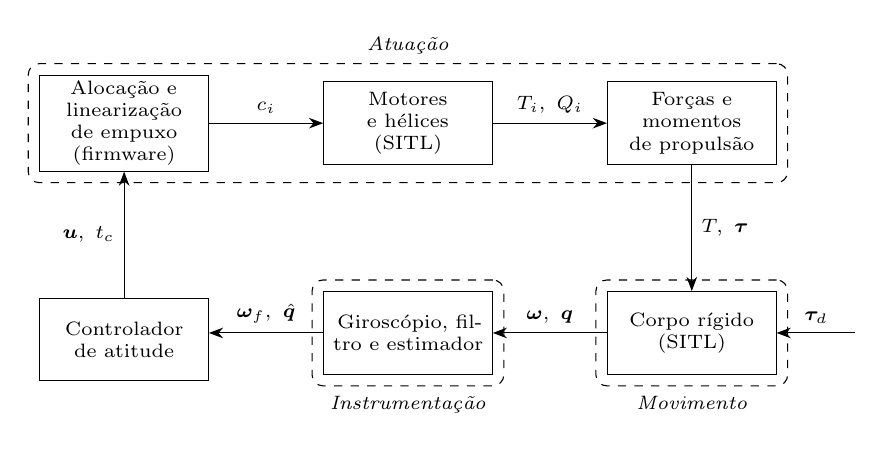
\begin{tikzpicture}[
    font=\scriptsize,
    bloco/.style={draw, rectangle, align=center, minimum height=1.05cm,
                  text width=2.0cm, inner sep=2pt},
    seta/.style={-{Stealth[length=1.8mm]}},
    grupo/.style={draw, dashed, rounded corners, inner sep=4pt},
    rotulo/.style={font=\scriptsize\itshape},
    node distance=1.6cm and 1.45cm,
]
    \node[bloco] (mix) {Alocação e linearização de empuxo\\(firmware)};
    \node[bloco, right=of mix] (mot) {Motores e hélices\\(SITL)};
    \node[bloco, right=of mot] (fm) {Forças e momentos de propulsão};
    \node[bloco, below=of fm] (cr) {Corpo rígido\\(SITL)};
    \node[bloco, below=of mot] (ins) {Giroscópio, filtro e estimador};
    \node[bloco, below=of mix] (ctl) {Controlador de atitude};

    \node[grupo, fit=(mix)(mot)(fm)] (gat) {};
    \node[rotulo, above] at (gat.north) {Atuação};
    \node[grupo, fit=(cr)] (gmv) {};
    \node[rotulo, below] at (gmv.south) {Movimento};
    \node[grupo, fit=(ins)] (gin) {};
    \node[rotulo, below] at (gin.south) {Instrumentação};

    \draw[seta] (ctl.north) -- node[left] {$\vetor{u},\ t_c$} (mix.south);
    \draw[seta] (mix) -- node[above] {$c_i$} (mot);
    \draw[seta] (mot) -- node[above] {$T_i,\ Q_i$} (fm);
    \draw[seta] (fm.south) -- node[right] {$T,\ \vetor{\tau}$} (cr.north);
    \draw[seta] (cr.west) -- node[above] {$\vetor{\omega},\ \vetor{q}$}
        (cr.west -| ins.east);
    \draw[seta] (ins.west) -- node[above] {$\vetor{\omega}_f,\ \hat{\vetor{q}}$}
        (ins.west -| ctl.east);
    \draw[seta] ($(cr.east)+(1.0,0)$) -- node[above] {$\vetor{\tau}_d$} (cr.east);
\end{tikzpicture}
\fonte{Elaborada pelo autor com base em \citeonline{fischer2025}.}
\end{figure}

A escolha das entradas e dos estados é a principal diferença em relação ao
minicurso. Lá, a entrada é o vetor das tensões aplicadas aos motores, e o
estado tem vinte componentes: a corrente e a velocidade de cada um dos quatro
motores, somadas aos doze estados do corpo rígido. Aqui, a entrada é a saída
do controlador de velocidade angular, o vetor de esforços normalizados
$\vetor{u} = [u_x\ u_y\ u_z]^{\mathsf{T}} \in [-1, 1]^3$ de
\eqref{eq:pid-taxa}, acompanhado do empuxo coletivo $t_c$ comandado pela malha
de altitude. É essa a grandeza que um \textit{backend} do
\codigo{AC\_CustomControl} entrega ao firmware (Seção~\ref{sec:customcontrol}),
e, portanto, a entrada do modelo de projeto. Os estados dos motores
desaparecem porque o SITL não os modela, como se mostra a seguir.

% ----------------------------------------------------------------------
\section{Subsistema de atuação}
\label{sec:atuacao}

\subsection{Conjunto motor--hélice}
\label{sec:motor-helice}

No modelo do minicurso, cada rotor é um motor de corrente contínua acoplado a
uma hélice. A hélice produz o empuxo $T_i = k_T\,\Omega_i^2$ e o torque de
reação $Q_i = k_Q\,\Omega_i^2$ da Seção~\ref{sec:modelo}, e o motor obedece
às equações elétrica e mecânica~\cite{fischer2025}
\begin{equation}
L_m\,\dot I_i = V_{m,i} - R_m\,I_i - K_e\,\Omega_i, \qquad
J_m\,\dot\Omega_i = K_\tau\,I_i - Q_i - B_m\,\Omega_i,
\label{eq:motor-cc}
\end{equation}
em que $I_i$ e $V_{m,i}$ são a corrente e a tensão do motor $i$, $L_m$ e $R_m$
a indutância e a resistência do enrolamento, $K_e$ e $K_\tau$ as constantes de
força contraeletromotriz e de torque, e $J_m$ e $B_m$ a inércia do rotor com
a hélice e o atrito viscoso. O comando do controlador eletrônico de
velocidade é a tensão normalizada $\delta_i = V_{m,i}/V_{\mathrm{bat}}$;
calculando-o a partir da tensão desejada e da tensão medida da bateria, obtém-se
a mesma tensão no motor qualquer que seja a carga da
bateria~\cite{fischer2025} --- ideia que reaparece na compensação de tensão do
firmware (Seção~\ref{sec:alocacao-firmware}).

No voo pairado, cada rotor sustenta um quarto do peso, e as
Equações~\eqref{eq:motor-cc} em regime fornecem o ponto de
equilíbrio~\cite{fischer2025}
\begin{equation}
\Omega_{\mathrm{eq}} = \sqrt{\frac{mg}{4\,k_T}}, \qquad
I_{\mathrm{eq}} = \frac{k_Q\,\Omega_{\mathrm{eq}}^2 + B_m\,\Omega_{\mathrm{eq}}}{K_\tau}, \qquad
V_{\mathrm{eq}} = R_m\,I_{\mathrm{eq}} + K_e\,\Omega_{\mathrm{eq}}.
\label{eq:motor-equilibrio}
\end{equation}
Em torno dele, as pequenas variações obedecem a
$L_m\,\delta\dot I = \delta V - R_m\,\delta I - K_e\,\delta\Omega$ e
$J_m\,\delta\dot\Omega = K_\tau\,\delta I - (2k_Q\Omega_{\mathrm{eq}} + B_m)\,\delta\Omega$.
A constante de tempo elétrica $L_m/R_m$ costuma ser bem menor que a mecânica;
desprezando-a (aproximação de quase regime
permanente~\cite{kokotovic1999}), $\delta I = (\delta V - K_e\,\delta\Omega)/R_m$, e o conjunto se
reduz ao modelo de primeira ordem apresentado no minicurso,
\begin{equation}
\frac{\delta\Omega(s)}{\delta V(s)} = \frac{k_m}{\tau_m\,s + 1}, \qquad
\tau_m = \frac{J_m}{K_\tau K_e/R_m + 2k_Q\Omega_{\mathrm{eq}} + B_m}, \qquad
k_m = \frac{K_\tau\,\tau_m}{R_m\,J_m},
\label{eq:motor-primeira-ordem}
\end{equation}
com o empuxo variando em $\delta T_i = 2k_T\,\Omega_{\mathrm{eq}}\,\delta\Omega_i$.
O arrasto da própria hélice, pelo termo $2k_Q\Omega_{\mathrm{eq}}$, contribui
para o amortecimento do motor. Em uma aeronave real, cada motor acrescenta,
assim, um polo em $-1/\tau_m$ entre o comando e o empuxo, cujo valor depende do
motor e da hélice e deve ser medido em bancada, como no procedimento
experimental descrito por \citeonline{fischer2025}.

Uma observação de método vale para quem parte do modelo completo de vinte
estados e deseja um modelo de projeto reduzido. Como as tensões atuam apenas
sobre as correntes, as linhas e as colunas dos motores na matriz linearizada
contêm todo o caminho da entrada até as forças; truncá-las anula a matriz de
entrada do modelo reduzido. A redução correta é a residualização dos estados
rápidos, por perturbação singular~\cite{kokotovic1999}: impõe-se $\dot I_i = \dot\Omega_i = 0$ e
substituem-se as relações estáticas resultantes, como se fez acima para a
corrente.

\subsection{O motor no SITL}
\label{sec:motor-sitl}

O modelo de multirrotor do SITL não tem estados de motor. O comando
$c_i \in [0, 1]$ é obtido do PWM pela faixa útil do motor
(\codigo{SIM\_FRM\_SPIN\_MIN} e \codigo{SIM\_FRM\_SPIN\_MAX}), passa por um
limitador de taxa e determina o empuxo pela teoria do momento, em função da
velocidade do escoamento induzido~\cite{ardupilot2026}:
\begin{equation}
T_i = \frac{1}{2}\,\rho\,A_e\,\left(V_s\,v_{\max}\right)^2
      \left[(1-e)\,c_i + e\,c_i^2\right],
\qquad
Q_i = 0{,}05\,D\,T_i\,c_i,
\label{eq:empuxo-sitl}
\end{equation}
em que $\rho$ é a densidade do ar, $A_e$ a área efetiva do disco de cada
rotor, $v_{\max}$ a velocidade máxima do escoamento e $V_s$ a razão entre a
tensão da bateria simulada e a nominal. A área $A_e$ e a velocidade $v_{\max}$
são calculadas pelo simulador a partir da corrente e da tensão de referência
no pairado (\codigo{SIM\_FRM\_REF\_AMP} e \codigo{SIM\_FRM\_REF\_VOLT}) e do
coletivo de pairado do modelo (\codigo{SIM\_FRM\_HOVR\_THR}); a
Equação~\eqref{eq:motor-sitl} é o caso $\rho = \rho_{\mathrm{ref}}$ e
$V_s = 1$ desta.

A expressão completa do simulador tem ainda um termo de escoamento de
entrada: do quadrado da velocidade de saída, $(V_s\,v_{\max})^2[\cdots]$, ela
subtrai o quadrado da velocidade axial $v_{e,i} \geq 0$ com que o ar entra no
rotor quando este sobe em relação ao ar --- por exemplo, pela própria rotação
do corpo~\cite{ardupilot2026}. Como $v_{e,i}$ é nula no pairado e entra ao
quadrado, a derivada do empuxo em relação a ela é nula no equilíbrio, e o
termo foi omitido em~\eqref{eq:empuxo-sitl}: ele não contribui para o modelo
linear, apenas para as respostas a velocidades angulares grandes.

O limitador de taxa (\codigo{SIM\_FRM\_SLEW\_MAX}) permite variar o comando
em até \SI{150}{\per\second}: a faixa inteira é percorrida em
\SI{6.7}{\milli\second}, menos de três períodos do laço de controle, e as
pequenas variações da regulação não chegam a acioná-lo. Na prática, o
atuador do SITL é um mapa estático do comando no empuxo --- o modelo do
minicurso com $\tau_m \to 0$. A ausência de dinâmica de atuador é uma das
razões pelas quais a planta simulada é mais fácil de controlar que uma
aeronave real, e fica registrada como discrepância conhecida, conforme as
hipóteses da Seção~\ref{sec:modelo}.

O torque de reação merece atenção. No modelo da hélice, $Q_i/T_i = k_Q/k_T$
é constante; no SITL, $Q_i/T_i = 0{,}05\,D\,c_i$ cresce com o comando. Para o
controle, o que importa não é essa razão total, e sim a razão incremental
\begin{equation}
\kappa' = \frac{\mathrm{d}Q_i}{\mathrm{d}T_i}
        = 0{,}05\,D\left(c_i + T_i\,\frac{\mathrm{d}c_i}{\mathrm{d}T_i}\right),
\label{eq:kappa-incremental}
\end{equation}
que, no pairado da aeronave simulada, vale \SI{0.0165}{\metre}, 1,66 vez a
razão total $\kappa = \SI{0.0100}{\metre}$. Uma mesma diferença de empuxo
produz, portanto, um torque de guinada 66\,\% maior do que o modelo de
$\kappa$ constante faria supor.

\subsection{Alocação e linearização de empuxo no firmware}
\label{sec:alocacao-firmware}

Do lado do firmware, os esforços e o coletivo são distribuídos entre os
motores pela biblioteca \codigo{AP\_MotorsMatrix}. No regime linear, longe da
saturação, a fração de empuxo pedida ao motor $i$ é
\begin{equation}
t_i = t_c + f_{x,i}\,u_x + f_{y,i}\,u_y + f_{z,i}\,u_z,
\label{eq:mistura}
\end{equation}
com os fatores de rolagem $\cos(\alpha_i + \ang{90})$, de arfagem
$\cos\alpha_i$ e de guinada $\pm 1$ (positivo para os rotores CCW),
normalizados de modo que o maior valor absoluto em cada eixo seja
0,5~\cite{ardupilot2026}. A Tabela~\ref{tab:fatores} mostra o resultado para
o quadrirrotor X. Em cada eixo, os fatores somam zero: um esforço de atitude
redistribui o empuxo sem alterar o total.

\begin{table}[htbp]
\centering
\caption{Posição, sentido de rotação e fatores de alocação dos motores do
quadrirrotor X.}
\label{tab:fatores}
\begin{tabular}{ccccccc}
\toprule
Motor & $\alpha_i$ & $(x_i,\ y_i)/\ell_{xy}$ & Sentido & $f_{x,i}$ & $f_{y,i}$ & $f_{z,i}$ \\
\midrule
M1 & \ang{45}   & $(+1,\ +1)$ & CCW & $-0{,}5$ & $+0{,}5$ & $+0{,}5$ \\
M2 & \ang{-135} & $(-1,\ -1)$ & CCW & $+0{,}5$ & $-0{,}5$ & $+0{,}5$ \\
M3 & \ang{-45}  & $(+1,\ -1)$ & CW  & $+0{,}5$ & $+0{,}5$ & $-0{,}5$ \\
M4 & \ang{135}  & $(-1,\ +1)$ & CW  & $-0{,}5$ & $-0{,}5$ & $-0{,}5$ \\
\bottomrule
\end{tabular}

\fonte{\citeonline{ardupilot2026}: \codigo{AP\_MotorsMatrix.cpp} e
\codigo{SIM\_Frame.cpp}.}
\end{table}

Antes de chegar ao motor, as frações $t_i$ passam por três transformações. A
primeira é um ganho de compensação $g_c = 1/(L_{\max}\,\rho_r)$. O fator
$L_{\max}$ corrige a tensão da bateria em relação a
\codigo{MOT\_BAT\_VOLT\_MAX}, e $\rho_r$ é a razão entre a densidade do ar
estimada e a do nível do mar; com eles, o mesmo esforço produz o mesmo empuxo
em qualquer condição de bateria e de altitude. A tensão usada em $L_{\max}$
não é a medida, que cai com a corrente, e sim uma estimativa da tensão de
repouso,
\begin{equation}
\hat V_r = V + I\,\hat R,
\label{eq:tensao-repouso}
\end{equation}
em que $V$ e $I$ são a tensão e a corrente medidas e $\hat R$ é a resistência
interna da bateria, que o monitor de bateria do firmware estima em voo a
partir das variações de tensão e de corrente~\cite{ardupilot2026}. A
compensação depende, portanto, de uma estimativa, e não da tensão
verdadeira, o que tem consequência no ponto de equilíbrio
(Seção~\ref{sec:modelo-linear}). A segunda é a inversa da curva de empuxo,
que no código inclui o próprio $L_{\max}$ e a razão de tensão
$v = \hat V_r/\codigo{MOT\_BAT\_VOLT\_MAX}$,
\begin{equation}
c = \frac{-(1-e) + \sqrt{(1-e)^2 + 4\,e\,L_{\max}\,t}}{2\,e\,v},
\label{eq:inversa-empuxo-codigo}
\end{equation}
e se reduz à Equação~\eqref{eq:linearizacao-empuxo} quando $L_{\max} = v = 1$;
como $g_c$ já divide $t$ por $L_{\max}$, os dois fatores se cancelam, e a
compensação de tensão que resta é o fator $1/v$ sobre o comando. A terceira é
o mapeamento na faixa
útil do motor e a conversão em PWM. Como o firmware e o simulador usam o mesmo
expoente da curva ($e = 0{,}65$) e a mesma faixa útil, a inversa do firmware
cancela a curva do SITL, e o empuxo de cada motor fica, com ótima aproximação,
proporcional à fração pedida:
\begin{equation}
T_i \approx k_t\,t_i, \qquad k_t = \frac{mg}{4\,t_h},
\label{eq:empuxo-linear}
\end{equation}
em que $t_h$ é o coletivo de pairado, que o firmware aprende em voo e grava
no parâmetro \codigo{MOT\_THST\_HOVER}. Assim, $k_t$ incorpora todas as
compensações sem que seja preciso conhecer $\rho$, a tensão da bateria ou os
detalhes da curva --- inclusive os erros das estimativas que o próprio
firmware usa nelas. A não linearidade residual vem de $\hat V_r$ não
coincidir com \codigo{MOT\_BAT\_VOLT\_MAX}: quando coincide, a inversa cancela
a curva; no voo analisado, a diferença altera os coeficientes de controle em
0,5\,\% (Seção~\ref{sec:modelo-linear}).

% ----------------------------------------------------------------------
\section{Forças e momentos de propulsão}
\label{sec:forcas-momentos}

O minicurso escreve as forças e os momentos de propulsão para a configuração
``$+$'', em que cada eixo de rolagem e de arfagem é
atuado por um par de motores com braço $\ell$~\cite{fischer2025}. Na
configuração X, os quatro motores participam dos dois eixos, com alavanca
$\ell_{xy} = \ell/\sqrt{2}$, como na matriz de alocação~\eqref{eq:alocacao}.
Levando a mistura~\eqref{eq:mistura} e o empuxo linear~\eqref{eq:empuxo-linear}
à matriz de alocação, com as posições e os fatores da
Tabela~\ref{tab:fatores}, cada esforço produz torque apenas no próprio eixo:
\begin{equation}
\tau_x = 2\,\ell_{xy}\,k_t\,u_x, \qquad
\tau_y = 2\,\ell_{xy}\,k_t\,u_y, \qquad
\tau_z = 2\,\kappa'\,k_t\,u_z.
\label{eq:torques-esforcos}
\end{equation}
Em rolagem, por exemplo, $\tau_x = -\sum_i y_i\,k_t\,f_{x,i}\,u_x$, e os
quatro produtos $-y_i f_{x,i}$ valem $+\ell_{xy}/2$. Em guinada, o torque é
a soma dos incrementos de torque de reação, $\kappa'\,k_t\,f_{z,i}\,u_z$, com
o sinal do sentido de rotação de cada rotor. O empuxo total depende apenas de
$t_c$, porque os fatores de cada eixo somam zero.

A razão entre as autoridades de controle em rolagem e em guinada é
$\ell_{xy}/\kappa' = 15$ em torque e, como $J_{zz} = 2J_{xx}$, cerca de 30 em
aceleração angular. Com a razão total $\kappa$, que supõe o torque de reação
proporcional ao empuxo, seriam 25 e 50: o modelo de $\kappa$ constante
superestima a assimetria entre os eixos.

% ----------------------------------------------------------------------
\section{Subsistema de movimento}
\label{sec:movimento}

No minicurso, a dinâmica de translação é escrita no referencial do corpo,
\begin{equation}
m\,\dot{\vetor{v}}_b = -\vetor{\omega}\times m\,\vetor{v}_b + \vetor{F}_p
                      + \vetor{F}_a + m\,\matriz{R}^{\mathsf{T}} g\,\vetor{e}_3,
\qquad \dot{\vetor{p}} = \matriz{R}\,\vetor{v}_b,
\label{eq:translacao-corpo}
\end{equation}
com $\vetor{F}_p = [0\ 0\ -T]^{\mathsf{T}}$ o empuxo e $\vetor{F}_a$ a força
aerodinâmica~\cite{fischer2025}, forma equivalente a~\eqref{eq:translacao},
escrita com a velocidade no referencial inercial. As duas formas são
corretas; o que não se pode é combiná-las. Com a velocidade no corpo, o empuxo
permanece no corpo, a gravidade entra rotacionada por $\matriz{R}^{\mathsf{T}}$
e a posição se obtém por $\matriz{R}\,\vetor{v}_b$; com a velocidade no
referencial inercial, é o empuxo que se rotaciona, por $\matriz{R}$, e
$\dot{\vetor{p}} = \vetor{v}$. Somar o empuxo já rotacionado para o
referencial inercial à gravidade rotacionada para o corpo produz um modelo cuja
linearização não reproduz $\delta\ddot x = -g\,\delta\theta$
de~\eqref{eq:linear}. No pairado, a translação não realimenta a atitude em
primeira ordem, e o restante do capítulo trata apenas da rotação.

A dinâmica de rotação que o SITL integra (\codigo{SIM\_Frame.cpp}) difere
de~\eqref{eq:rotacao-euler} em dois pontos. O termo giroscópico
$\vetor{\omega}\times\matriz{J}\vetor{\omega}$ não é modelado
(Seção~\ref{sec:sitl}), e a força de cada rotor inclui um \emph{arrasto de
momento}: o rotor, ao se deslocar em relação ao ar, sofre uma força contrária
à sua velocidade, proporcional à vazão de ar que ele processa. Com
$\vetor{r}_i$ a posição do rotor $i$ e
$\vetor{v}_i = \vetor{\omega}\times\vetor{r}_i$ a sua velocidade devida à
rotação do corpo, a dinâmica é
\begin{equation}
\dot{\vetor{\omega}} = \matriz{J}^{-1}\sum_{i=1}^{4}\left[
    \vetor{r}_i\times\left(-T_i\,\vetor{e}_3 - k_{md,i}\,\vetor{v}_i\right)
    + s_i\,Q_i\,\vetor{e}_3\right]
  - a_r\,\vetor{\omega} + \vetor{a}_{\mathrm{tw}},
\qquad
k_{md,i} = C_{md}\sqrt{\rho\,A_p\,T_i},
\label{eq:rotacao-sitl-completa}
\end{equation}
em que $s_i = \pm 1$ é o sentido de rotação do rotor (positivo para CCW),
$C_{md}$ é o coeficiente de arrasto de momento (\codigo{SIM\_FRM\_MDRAG},
0,2), $A_p$ a área real do disco de cada rotor e $a_r$ a resistência
rotacional explícita do modelo, que vale \SI{0.058}{\per\second} com o valor
padrão de \codigo{SIM\_FRM\_ROT\_RATE}.

O arrasto de momento é um amortecimento aerodinâmico. Uma velocidade de
rolagem $p$ desloca o rotor $i$ na vertical com velocidade $p\,y_i$, e a força
de arrasto resultante produz o torque $-k_{md}\,y_i^2\,p$; uma velocidade de
guinada $r$ desloca o rotor no plano com velocidade de módulo $r\,\ell$, e o
torque é $-k_{md}\,\ell^2\,r$. Somando os quatro rotores,
\begin{equation}
a_{md,x} = a_{md,y} = \frac{4\,k_{md}\,\ell_{xy}^2}{J_{xx}}, \qquad
a_{md,z} = \frac{4\,k_{md}\,\ell^2}{J_{zz}},
\label{eq:amortecimento-md}
\end{equation}
iguais entre si na aeronave simulada, porque $\ell^2 = 2\ell_{xy}^2$ e
$J_{zz} = 2J_{xx}$. É esse termo, e não a resistência rotacional $a_r$, que
domina o amortecimento: $a_{md} = \SI{1.93}{\per\second}$ contra
$a_r = \SI{0.058}{\per\second}$. A constante de tempo de \SI{17}{\second}
associada a $a_r$ cai, com o arrasto de momento, para \SI{0.50}{\second}.

A origem desse amortecimento, porém, não é a mesma nos três eixos. Em
guinada, a velocidade $r\,\ell$ dos rotores é paralela ao plano do disco, e a
força correspondente é o arrasto de momento propriamente dito, que um rotor
real também sofre. Em rolagem e arfagem, a velocidade $p\,y_i$ é
\emph{axial}, e o simulador aplica a ela o mesmo coeficiente, porque modela o
arrasto de momento como isotrópico. Em um rotor real, uma velocidade axial age
por outro mecanismo: altera o escoamento através do disco e, com ele, o
empuxo, já em primeira ordem. No SITL, esse efeito aparece apenas pelo termo
em $v_{e,i}^2$ da Seção~\ref{sec:motor-sitl}, de derivada nula no pairado, e o
próprio código-fonte descreve a componente axial do arrasto de momento como
um artifício para compensar essa deficiência, introduzido para que a
aeronave não suba com velocidade irreal quando o acelerador é comandado
diretamente pelo piloto~\cite{ardupilot2026}. O valor de $a$ em rolagem e
arfagem é, assim, um efeito colateral desse ajuste, e não uma previsão
física. Para o projeto, isso significa que $a$ não pode ser transposto do
simulador para uma aeronave real: lá, ele precisa ser identificado
(Seção~\ref{sec:validacao-identificacao}).

A cinemática de atitude é a da Equação~\eqref{eq:cinematica-euler}, a matriz
$\matriz{S}$ do minicurso~\cite{fischer2025}; no pairado, ela se reduz a
$\dot\phi = p$, $\dot\theta = q$ e $\dot\psi = r$.

% ----------------------------------------------------------------------
\section{Ponto de equilíbrio e modelo linear de atitude}
\label{sec:modelo-linear}

Como na Parte~3 do minicurso, o modelo é linearizado em torno do voo pairado,
com $\vetor{\omega} = \vetor{0}$, $\phi = \theta = 0$, $\vetor{u} = \vetor{0}$
e o coletivo que equilibra o peso. Sem estados de motor, o equilíbrio se
reduz a encontrar o coletivo $t_h$ para o qual a cadeia da
Seção~\ref{sec:atuacao} produz $\sum_i T_i = mg$, o que o programa faz por
bisseção, na altitude dos ensaios, \SI{599}{\metre} acima do nível do mar, e
com a queda de tensão da bateria simulada sob a corrente de pairado.

Esse cálculo depende de uma grandeza que não pertence à física, e sim ao
firmware: a tensão de repouso estimada $\hat V_r$ com que o ganho de
compensação é calculado~\eqref{eq:tensao-repouso}. Tomando-a igual à tensão
sem carga da bateria simulada, \SI{12.6}{\volt}, como seria se a resistência
interna fosse estimada sem erro, o coletivo previsto é $t_h = 0{,}3775$, 2\,\%
acima dos $0{,}3702$ aprendidos pelo firmware no mesmo voo. O registro do voo
mostra a origem da diferença. O estimador de resistência, que só se atualiza
quando a corrente varia, chegou ao pairado com $\hat R = \SI{0.0045}{\ohm}$,
menos da metade dos \SI{0.010}{\ohm} da bateria simulada
(\codigo{SIM\_FRM\_BAT\_RES}), e manteve esse valor durante todo o pairado.
Com isso, a tensão de repouso estimada ficou em $\hat V_r = \SI{12.44}{\volt}$,
e o fator registrado $L_{\max}$ (\codigo{MOTB.LiftMax}), em 0,954, contra
0,974 com a tensão sem carga. Com o $\hat V_r$ do registro, o programa
reproduz esse $L_{\max}$ e prevê $t_h = 0{,}3703$, a 0,03\,\% do valor
aprendido. O modelo físico estava correto; faltava reproduzir a estimativa
que o firmware efetivamente usa.

A consequência para o projeto é que os coeficientes de controle dependem de
$\hat R$. Como o estimador se atualiza a cada variação de corrente, essa
estimativa muda ao longo do voo e de um voo para outro --- no voo analisado,
subiu para \SI{0.0068}{\ohm} até o pouso ---, e um erro nela desloca o
coletivo de pairado e, na mesma proporção, $b_x$ e $b_y$: 2\,\% neste caso.
A forma de acompanhar essa variação já está na
Equação~\eqref{eq:empuxo-linear}: o $t_h$ aprendido é obtido pelo mesmo
firmware, sob a mesma compensação, e as expressões que o usam incorporam a
estimativa vigente, com o atraso do aprendizado, sem que seja preciso
conhecê-la. O comando de pairado de cada motor, $c_h = 0{,}569$, não depende
de $\hat V_r$, porque é fixado pelo empuxo que o simulador precisa produzir;
fica um pouco acima do valor da Tabela~\ref{tab:aeronave}, calculado nas
condições de referência do modelo.

A linearização é feita, como no minicurso, por diferenças centrais: cada
componente de $\vetor{\omega}$ e de $\vetor{u}$ é perturbada de $\pm 10^{-4}$
em torno do equilíbrio, e a cadeia completa --- mistura, compensação,
linearização de empuxo, motor e corpo rígido --- é reavaliada, com o
$\hat V_r$ do registro. O resultado é
\begin{equation}
\dot{\vetor{\omega}} = -a\,\vetor{\omega} + \matriz{B}_\omega\,\vetor{u} + \vetor{d},
\qquad
\matriz{B}_\omega = \operatorname{diag}(b_x,\ b_y,\ b_z),
\label{eq:modelo-taxa}
\end{equation}
com $a = \SI{1.988}{\per\second}$, $b_x = b_y = \SI{430.0}{\radian\per\second\squared}$,
$b_z = \SI{14.37}{\radian\per\second\squared}$ e
$\vetor{d} = \matriz{J}^{-1}\vetor{\tau}_d$ a perturbação expressa em
aceleração angular. Os termos fora da diagonal das matrizes linearizadas são
nulos: no pairado, os três eixos estão desacoplados. As expressões fechadas
das Seções~\ref{sec:forcas-momentos} e~\ref{sec:movimento},
\begin{equation}
b_x = b_y = \frac{m\,g\,\ell_{xy}}{2\,t_h\,J_{xx}}, \qquad
b_z = \frac{2\,\kappa'\,k_t}{J_{zz}} = \frac{\kappa'\,m\,g}{2\,t_h\,J_{zz}}, \qquad
a = a_{md} + a_r,
\label{eq:coeficientes-fechados}
\end{equation}
reproduzem a linearização numérica com diferença de 0,5\,\% em $b_x$, $b_y$
e $b_z$ e de menos de 0,1\,\% em $a$. A
Tabela~\ref{tab:modelo-linear} reúne os valores.

\begin{table}[htbp]
\centering
\caption{Parâmetros do modelo linear de atitude da aeronave simulada no voo
pairado.}
\label{tab:modelo-linear}
\begin{tabular}{llr}
\toprule
Grandeza & Símbolo & Valor \\
\midrule
Densidade do ar a \SI{599}{\metre}                 & $\rho$     & \SI{1.156}{\kilogram\per\cubic\metre} \\
Resistência da bateria, estimada / simulada        & $\hat R$   & \SI{0.0045}{\ohm} / \SI{0.010}{\ohm} \\
Tensão de repouso estimada pelo firmware           & $\hat V_r$ & \SI{12.44}{\volt} \\
Coletivo de pairado, previsto / aprendido          & $t_h$      & 0,3703 / 0,3702 \\
Comando de cada motor no pairado                   & $c_h$      & 0,569 \\
Empuxo de cada motor no pairado                    & $T_h$      & \SI{7.355}{\newton} \\
Empuxo por unidade de fração de empuxo             & $k_t$      & \SI{19.86}{\newton} \\
Razão total entre torque de reação e empuxo        & $\kappa$   & \SI{0.0100}{\metre} \\
Razão incremental                                  & $\kappa'$  & \SI{0.0165}{\metre} \\
Coeficiente de arrasto de momento por rotor        & $k_{md}$   & \SI{0.181}{\newton\second\per\metre} \\
Amortecimento por arrasto de momento               & $a_{md}$   & \SI{1.930}{\per\second} \\
Resistência rotacional do modelo                   & $a_r$      & \SI{0.058}{\per\second} \\
Amortecimento total                                & $a$        & \SI{1.988}{\per\second} \\
Eficácia de controle em rolagem e arfagem          & $b_x = b_y$ & \SI{430.0}{\radian\per\second\squared} \\
Eficácia de controle em guinada                    & $b_z$      & \SI{14.37}{\radian\per\second\squared} \\
\bottomrule
\end{tabular}

\fonte{Calculados por \codigo{modelagem/modelo\_sitl.py} a partir dos
parâmetros gravados no ensaio \codigo{vento/rajada/nativo/2026-10-27\_214349},
o mesmo de que parte o projeto (Capítulo~\ref{cap:projeto}), do $\hat V_r$ do
registro do mesmo voo (\codigo{BAT.VoltR}) e do
código-fonte~\cite{ardupilot2026}.}
\nota{\raggedright Coeficientes por linearização numérica; $k_t$ e $\kappa'$
pelas Equações~\eqref{eq:empuxo-linear} e~\eqref{eq:kappa-incremental} com o
$t_h$ previsto. Com a tensão sem carga da bateria simulada no lugar de
$\hat V_r$, o programa prevê $t_h = 0{,}3775$,
$b_x = b_y = \SI{420.9}{\radian\per\second\squared}$ e
$b_z = \SI{14.06}{\radian\per\second\squared}$.}
\end{table}

Com a cinemática do pairado, cada eixo de atitude é descrito por dois estados.
Para a rolagem, com $\vetor{x}_\phi = [\phi\ \ p]^{\mathsf{T}}$,
\begin{equation}
\dot{\vetor{x}}_\phi =
\begin{bmatrix} 0 & 1 \\ 0 & -a \end{bmatrix} \vetor{x}_\phi +
\begin{bmatrix} 0 \\ b_x \end{bmatrix} u_x +
\begin{bmatrix} 0 \\ 1 \end{bmatrix} d_x,
\qquad
\frac{\Phi(s)}{U_x(s)} = \frac{b_x}{s\,(s + a)},
\label{eq:modelo-eixo}
\end{equation}
e analogamente para a arfagem e a guinada, com $b_y$ e $b_z$. Em relação ao
duplo integrador~\eqref{eq:duplo-integrador}, mudam duas coisas. A entrada
passa a ser o esforço normalizado, e $1/J_{xx}$ dá lugar à eficácia $b_x$, que
reúne a mistura, a linearização de empuxo, o braço e a inércia. E um dos
polos sai da origem para $-a \approx \SI{-2}{\radian\per\second}$. Esse polo
fica muito abaixo da banda passante da malha de velocidade angular, de
algumas dezenas de radianos por segundo, e pouco altera o rastreamento; ele
pesa, porém, na resposta a perturbações lentas, sobretudo em guinada, em que
a eficácia é 30 vezes menor. A perturbação $d$ entra exatamente na escala em
que o injetor de perturbações dos ensaios a aplica, em
\si{\radian\per\second\squared}.

Discretizado com segurador de ordem zero~\cite{franklin1998} no período $T_s$
do laço de controle, o modelo~\eqref{eq:modelo-eixo} fica
\begin{equation}
\vetor{x}_{\phi,k+1} =
\begin{bmatrix} 1 & \beta \\ 0 & \mathrm{e}^{-aT_s} \end{bmatrix} \vetor{x}_{\phi,k} +
b_x \begin{bmatrix} (T_s - \beta)/a \\ \beta \end{bmatrix} u_{x,k},
\qquad
\beta = \frac{1 - \mathrm{e}^{-aT_s}}{a},
\label{eq:modelo-eixo-discreto}
\end{equation}
que, com $aT_s = 0{,}005$, difere do duplo integrador
discretizado~\eqref{eq:discreto} apenas na terceira casa decimal.

% ----------------------------------------------------------------------
\section{Instrumentação}
\label{sec:instrumentacao}

O controlador não recebe $\vetor{\omega}$, e sim a velocidade angular medida
pelo giroscópio e filtrada por um passa-baixas de segunda ordem do tipo
Butterworth~\cite{butterworth1930}, com frequência de corte de
\SI{20}{\hertz} (\codigo{INS\_GYRO\_FILTER}). Na frequência $f < f_c$, o
filtro atrasa a fase em
$\arctan\!\left[\sqrt{2}\,(f/f_c)\big/\left(1 - (f/f_c)^2\right)\right]$:
\ang{24} a \SI{5.7}{\hertz}, a ordem da banda passante da malha de
velocidade angular, e \ang{43} a \SI{10}{\hertz}. Nos ensaios-base, o ruído
do giroscópio proporcional ao acelerador está desligado
(\codigo{SIM\_GYR1\_RND} nulo), e resta só o ruído mínimo fixo do simulador,
da ordem de \SI{0.01}{\degree\per\second} (Seção~\ref{sec:sensores-sitl}),
condição mais favorável que a de uma aeronave real, sobretudo para
observadores de perturbação; os cenários de ruído do
Capítulo~\ref{cap:resultados} o ligam em quatro níveis.

Entre a amostra do giroscópio e o efeito do comando no modelo físico, o modelo
considera o segurador de ordem zero do laço de controle: o esforço calculado
em um laço já vale durante os três passos seguintes do modelo físico, de
\SI{1200}{\hertz}, até o próximo laço, de \SI{400}{\hertz}, porque o SITL
integra o modelo físico com a última saída dos motores antes de gerar a
amostra seguinte do giroscópio~\cite{ardupilot2026}. O ângulo, ao contrário,
chega ao controlador com um laço de atraso, e a validação da
Seção~\ref{sec:validacao-identificacao} usa essa temporização. Acrescentando
à simulação mais um laço de atraso na atuação (\SI{2.5}{\milli\second}), a
resposta em frequência de rolagem e arfagem passa a diferir da do SITL em
\SI{0.57}{\decibel} de ganho, na mediana, em até
\SI{2.1}{\decibel} e em até \ang{7.7} de fase,
contra \SI{0.08}{\decibel}, \SI{1.3}{\decibel} e \ang{5.8} sem ele; no tempo, o desvio máximo do modelo passa de 2,3\,\% abaixo
a 0,3\,\% acima do valor do SITL para 0,8\,\% a 2,6\,\% acima. Não há,
portanto, atraso de atuação apreciável além do segurador.

% ----------------------------------------------------------------------
\section{Validação e identificação}
\label{sec:validacao-identificacao}

O modelo~\eqref{eq:modelo-taxa} foi confrontado com os ensaios em SITL de
duas formas: no domínio do tempo, simulando a malha fechada nos ensaios de
torque em pulso e em degrau, e no domínio da frequência, nas varreduras de
torque, comparando a resposta em frequência da malha fechada e identificando
os parâmetros da planta. Todos os ensaios são do mesmo lote, com os ganhos da
Tabela~\ref{tab:ganhos}.

\subsection{Malha fechada no domínio do tempo}
\label{sec:validacao-tempo}

Um segundo programa (\codigo{modelagem/validacao.py}) simula, para cada
ensaio, a malha fechada de cada eixo perturbado: a planta de primeira ordem
com o ângulo, integrada a \SI{1200}{\hertz} como no SITL; o filtro do
giroscópio; o controlador de ângulo --- com o controlador de raiz
quadrada~\eqref{eq:sqrt-controller} no PID nativo e só o ganho proporcional
no \textit{backend} de exemplo, como no código de cada um --- e o controlador
de velocidade angular~\eqref{eq:pid-taxa}, com os filtros e o limite do
integrador, a \SI{400}{\hertz}. Os ganhos são lidos dos parâmetros gravados
no próprio voo, e $a$ e $b$ vêm da linearização da
Seção~\ref{sec:modelo-linear}, com a tensão de repouso que o firmware estimou
naquele voo. A entrada é o torque que o injetor registrou no ensaio, e as
métricas são calculadas pelo mesmo código e na mesma janela da análise dos
ensaios (Seção~\ref{sec:metricas}); modelo e SITL são comparados, assim,
número a número. Não há ajuste: nenhum parâmetro do modelo é escolhido para
aproximar os resultados. O ângulo chega ao controlador com um laço de atraso,
como o firmware o entrega (Seção~\ref{sec:instrumentacao}), e o esforço
calculado em um laço já age no modelo físico até o laço seguinte.

\begin{table}[htbp]
\centering
\caption{Métricas de rejeição de torque no SITL e no modelo linear em malha
fechada.}
\label{tab:validacao}
\small
\setlength{\tabcolsep}{4pt}
% Gerada por modelagem/validacao.py — nao editar a mao.
\begin{tabular}{lllrrrrrr}
\toprule
 & & & \multicolumn{2}{c}{Desvio máx. (\si{\degree})} & \multicolumn{2}{c}{Recuperação (\si{\second})} & \multicolumn{2}{c}{RMSE (\si{\degree})} \\
\cmidrule(lr){4-5}\cmidrule(lr){6-7}\cmidrule(lr){8-9}
Eixo & Torque & Controlador & SITL & Modelo & SITL & Modelo & SITL & Modelo \\
\midrule
Rolagem & pulso & nativo & 0,90 & 0,89 & 1,32 & 1,40 & 0,229 & 0,230 \\
Rolagem & pulso & \codigo{cc\_pid} & 0,91 & 0,90 & 1,21 & 1,29 & 0,224 & 0,224 \\
Arfagem & pulso & nativo & 0,93 & 0,92 & 1,25 & 1,34 & 0,233 & 0,233 \\
Arfagem & pulso & \codigo{cc\_pid} & 0,94 & 0,93 & 1,25 & 1,30 & 0,233 & 0,234 \\
Guinada & pulso & nativo & 6,06 & 6,04 & 0,35 & 0,35 & 1,678 & 1,672 \\
Guinada & pulso & \codigo{cc\_pid} & 5,70 & 5,67 & 0,35 & 0,35 & 1,563 & 1,554 \\
Rolagem & degrau & nativo & 0,60 & 0,59 & 2,25 & 2,09 & 0,070 & 0,069 \\
Rolagem & degrau & \codigo{cc\_pid} & 0,61 & 0,60 & 2,09 & 2,10 & 0,070 & 0,069 \\
Arfagem & degrau & nativo & 0,61 & 0,61 & 2,15 & 2,14 & 0,073 & 0,072 \\
Arfagem & degrau & \codigo{cc\_pid} & 0,62 & 0,62 & 2,22 & 2,10 & 0,073 & 0,072 \\
Guinada & degrau & nativo & 2,56 & 2,56 & 22,18 & 22,78 & 0,847 & 0,846 \\
Guinada & degrau & \codigo{cc\_pid} & 2,56 & 2,56 & 22,09 & 22,84 & 0,847 & 0,847 \\
Rolagem (3 eixos) & pulso & nativo & 0,90 & 0,89 & 1,29 & 1,37 & 0,228 & 0,226 \\
Rolagem (3 eixos) & pulso & \codigo{cc\_pid} & 0,91 & 0,90 & 1,29 & 1,34 & 0,229 & 0,227 \\
Arfagem (3 eixos) & pulso & nativo & 0,92 & 0,92 & 1,31 & 1,36 & 0,234 & 0,237 \\
Arfagem (3 eixos) & pulso & \codigo{cc\_pid} & 0,93 & 0,93 & 1,27 & 1,36 & 0,235 & 0,237 \\
Guinada (3 eixos) & pulso & nativo & 6,03 & 6,02 & 0,35 & 0,35 & 1,669 & 1,665 \\
Guinada (3 eixos) & pulso & \codigo{cc\_pid} & 6,02 & 6,02 & 0,35 & 0,35 & 1,666 & 1,665 \\
Rolagem (3 eixos) & degrau & nativo & 0,59 & 0,59 & 2,30 & 2,09 & 0,056 & 0,055 \\
Rolagem (3 eixos) & degrau & \codigo{cc\_pid} & 0,61 & 0,60 & 2,21 & 2,09 & 0,056 & 0,055 \\
Arfagem (3 eixos) & degrau & nativo & 0,61 & 0,61 & 2,28 & 2,14 & 0,058 & 0,057 \\
Arfagem (3 eixos) & degrau & \codigo{cc\_pid} & 0,62 & 0,62 & 2,23 & 2,10 & 0,058 & 0,057 \\
Guinada (3 eixos) & degrau & nativo & 2,54 & 2,55 & 22,14 & 22,78 & 0,842 & 0,845 \\
Guinada (3 eixos) & degrau & \codigo{cc\_pid} & 2,54 & 2,56 & 22,24 & 22,88 & 0,843 & 0,848 \\
\bottomrule
\end{tabular}


\fonte{Elaborada pelo autor, por \codigo{modelagem/validacao.py}.}
\end{table}

A entrada da simulação é o torque como o injetor efetivamente o aplicou: o
valor de cada escrita da mensagem \codigo{WND}, segurado até a escrita
seguinte, no instante registrado. O perfil nominal não serviria, porque o laço
do injetor roda a cerca de \SI{44}{\hertz}, e não aos \SI{50}{\hertz}
pedidos, e a duração efetiva do pulso nominal de \SI{0.3}{\second} variou de
300 a \SI{338}{\milli\second} entre os voos deste lote (em todos os voos
válidos, até \SI{344}{\milli\second}; Seção~\ref{sec:injetor}).

A Tabela~\ref{tab:validacao} e a Figura~\ref{fig:validacao-tempo} mostram o
resultado, em 24 comparações, que incluem os ensaios simultâneos nos três
eixos. O desvio máximo é reproduzido com diferença de no máximo 2,3\,\%, no
pulso e no degrau sustentado, e o erro quadrático médio, com no máximo
2,2\,\%. Em rolagem e arfagem, o desvio máximo do modelo fica entre 2,3\,\%
abaixo e 0,3\,\% acima do valor do SITL; em guinada, a diferença não passa de
0,7\,\%. O tempo de recuperação concorda com diferença de no máximo 9,2\,\%
no degrau sustentado; em guinada, a recuperação lenta é reproduzida em
detalhe, \SI{22.8}{\second} no modelo contra \SI{22.2}{\second} no SITL. No
pulso de rolagem e arfagem, o modelo recupera de 3\,\% a 7\,\% mais devagar.
A recuperação do pulso é, de todas, a métrica mais sensível: quando a resposta
tem um pequeno sobressinal de amplitude próxima ao limiar de 10\,\% do pico,
uma diferença mínima decide se o erro volta ou não a cruzar o limiar, e a
recuperação muda de forma descontínua --- é o que ocorre no pulso de guinada
quando se acrescenta à simulação um laço de atraso na atuação: com o desvio
máximo praticamente igual, a recuperação do modelo salta de 0,35 para cerca
de \SI{0.55}{\second}.

\begin{figure}[htbp]
\centering
\caption{Erro de atitude no SITL e no modelo linear em malha fechada, com o
PID nativo, nos ensaios de torque em pulso e em degrau.}
\label{fig:validacao-tempo}
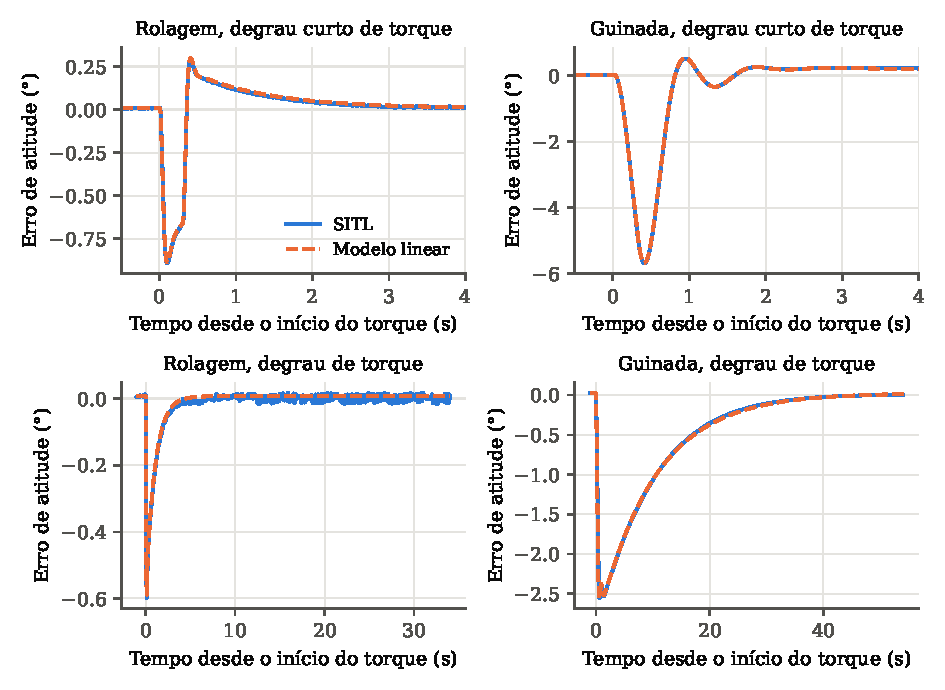
\includegraphics[width=\textwidth]{figuras/validacao_tempo}
\fonte{Elaborada pelo autor, por \codigo{modelagem/validacao.py}.}
\end{figure}

A simulação explica também a recuperação lenta da guinada. Desprezando os
filtros, a malha fechada de um eixo com o controlador de ângulo proporcional
de ganho $k$ e o PI de velocidade angular tem o polinômio característico
\begin{equation}
s^3 + (a + b\,k_P)\,s^2 + b\,(k_P\,k + k_I)\,s + b\,k_I\,k,
\label{eq:polinomio-malha}
\end{equation}
que, em guinada, tem um polo real lento próximo de $-k_I/k_P$, praticamente
independente de $a$ e de $b$. Com os ganhos gravados no voo, que a
Tabela~\ref{tab:ganhos} traz arredondados, as raízes são $-8{,}20$,
$-2{,}42$ e $\SI{-0.101}{\per\second}$, e o polo lento
tem constante de tempo de \SI{9.9}{\second}, para $k_P/k_I = \SI{10}{\second}$.
Uma exponencial com essa constante leva $\tau\ln 10 = \SI{22.8}{\second}$ para
cair a 10\,\% do pico, exatamente o tempo de recuperação do modelo e,
com 3\,\% de diferença no nativo e 3,4\,\% no \textit{backend} de exemplo, o
do SITL. A recuperação lenta não é, portanto, uma
limitação da planta, e sim consequência direta da razão $k_I = k_P/10$ que o
AutoTune impõe em guinada (Seção~\ref{sec:autotune}). Para o torque aplicado
como perturbação, o zero do PI em $-k_I/k_P$ não cancela esse polo, ao
contrário do que ocorre para um degrau de referência.

\subsection{Domínio da frequência}
\label{sec:validacao-frequencia}

Nas varreduras de torque, a resposta em frequência da perturbação para o
ângulo foi estimada pela Equação~\eqref{eq:frf}, no SITL e na simulação
alimentada pelo mesmo torque, com o mesmo método; nos dois casos, a entrada é
o torque registrado na mensagem \codigo{WND}, segurado entre as escritas do
injetor. Nos pontos em que a
coerência do SITL é de pelo menos 0,8 --- de 0,4 a \SI{9.6}{\hertz} em
rolagem e arfagem e de 0,2 a \SI{4.8}{\hertz} em guinada, praticamente toda
a faixa das varreduras ---, o modelo reproduz o ganho com diferença mediana
de no máximo \SI{0.08}{\decibel} e máxima de \SI{1.3}{\decibel}, e a fase
com diferença máxima de \ang{5.8}, em rolagem e arfagem; em guinada, as
diferenças são de \SI{0.05}{\decibel}, \SI{0.9}{\decibel} e \ang{3.2}
(Figura~\ref{fig:validacao-freq}), nos dois controladores.

\begin{figure}[htbp]
\centering
\caption{Resposta em frequência do torque para o ângulo com o PID nativo, no
SITL (pontos com coerência de pelo menos 0,8) e no modelo linear.}
\label{fig:validacao-freq}
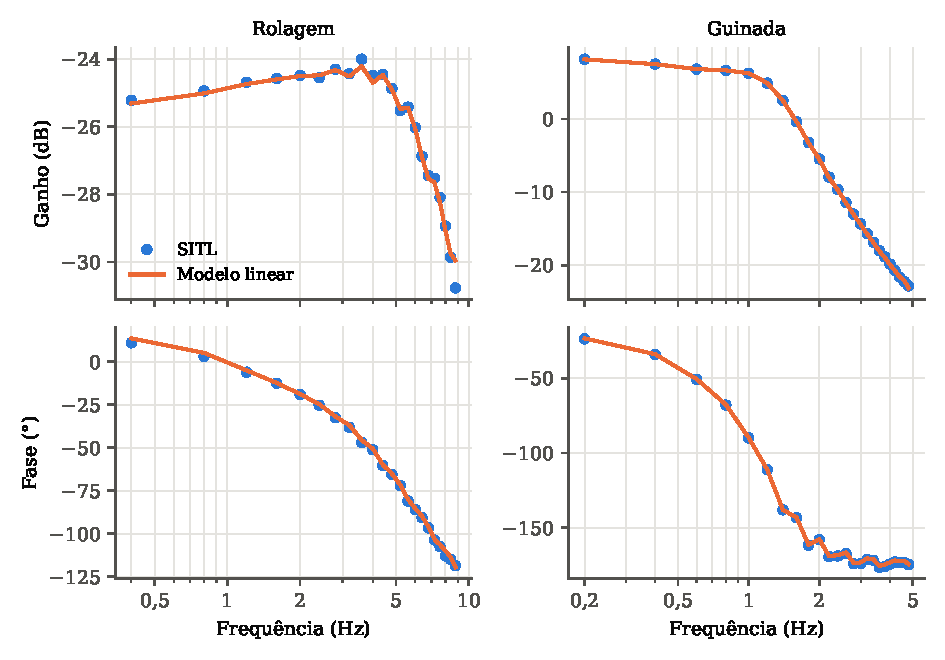
\includegraphics[width=\textwidth]{figuras/validacao_freq}
\fonte{Elaborada pelo autor, por \codigo{modelagem/validacao.py}.}
\end{figure}

As mesmas varreduras permitem identificar a planta, como prevê a
Seção~\ref{sec:identificacao}, apesar de a malha estar fechada. O torque
injetado $d$ é externo à malha e, como o ruído do giroscópio simulado é
mínimo e independente dele, não se correlaciona com nenhuma outra entrada. Dividindo a transformada de
$\dot\omega = -a\,\omega + b\,u + d$ pela de $d$, obtém-se
\begin{equation}
\mathrm{j}2\pi f\;\hat T_{d\omega}(f) - 1 = -a\,\hat T_{d\omega}(f) + b\,\hat T_{du}(f),
\label{eq:identificacao-planta}
\end{equation}
em que $\hat T_{d\omega}$ e $\hat T_{du}$ são as respostas em frequência de
$d$ para a velocidade angular e para o esforço, estimadas pelo método de
Welch contra o torque injetado. A equação é linear em $a$ e $b$, que são
obtidos por mínimos quadrados sobre os pontos de coerência de pelo menos 0,8
nas duas estimativas, separando as partes real e imaginária. A velocidade
angular registrada é a filtrada pelo passa-baixas do giroscópio, cuja
resposta em frequência é descontada de $\hat T_{d\omega}$, e os sinais são
lidos do registro a \SI{400}{\hertz}, com o torque segurado entre as escritas
do injetor, como no SITL.

Nas quatro varreduras de rolagem e arfagem, com os dois controladores, a
faixa útil vai de 0,4 a cerca de \SI{9.5}{\hertz}, com 23 ou 24 pontos. Com
$a$ e $b$ livres, $b$ sai entre 440 e \SI{446}{\radian\per\second\squared},
de 2,4\,\% a 3,6\,\% acima do previsto, mas $a$ sai negativo, entre $-1{,}5$
e $\SI{-0.06}{\per\second}$, sem significado físico. Na faixa em que a coerência
é alta, o termo $a\,\hat T_{d\omega}$ é pequeno diante de
$\mathrm{j}2\pi f\,\hat T_{d\omega}$, e os dois parâmetros se compensam: as
varreduras não identificam $a$. Fixando $a$ no valor do modelo,
$\SI{1.988}{\per\second}$, a eficácia identificada fica entre 429,5 e
\SI{432.1}{\radian\per\second\squared}, a no máximo 0,5\,\% dos
\SI{430.0}{\radian\per\second\squared} previstos.

Em guinada, a varredura começa em \SI{0.2}{\hertz}, onde $2\pi f$ é da
ordem de $a$, e os dois parâmetros se separam. Nas duas varreduras,
identificam-se $a$ entre 2,01 e $\SI{2.07}{\per\second}$, de 1\,\% a
4\,\% acima dos $\SI{1.988}{\per\second}$ previstos, e
$b_z = \SI{14.6}{\radian\per\second\squared}$, 1,4\,\% a 1,8\,\% acima
dos \SI{14.37}{\radian\per\second\squared} do modelo. As eficácias de
controle dos três eixos, parâmetros de que o projeto mais depende, estão
confirmadas dentro de 2\,\%, e o amortecimento, identificado diretamente em
guinada, onde as varreduras o alcançam, e indiretamente, pelas respostas no
tempo, em rolagem e arfagem.

% ======================================================================
%  CAPÍTULO 5 — PROJETO E IMPLEMENTAÇÃO DO CONTROLADOR
%
%  Ainda não escrito. Existe para que a numeração dos capítulos seguintes
%  bata com a Seção "Organização do trabalho" e com as referências cruzadas.
% ======================================================================
\chapter{Projeto e implementação do controlador}
\label{cap:projeto}

\pendente{Projeto do controlador de atitude sobre o modelo da
Seção~\ref{sec:modelo-linear}: LQR com ação integral, com a alocação de polos
como alternativa, margens de estabilidade e discretização a
\SI{400}{\hertz}; observador de estado estendido para estimação e
compensação da perturbação; implementação como novo \textit{backend} do
\codigo{AC\_CustomControl} (as quatro edições do \textit{framework} já
estão localizadas e listadas no modelo de configuração
\codigo{cc\_lqr.yaml.exemplo}), com ganhos expostos
como parâmetros, registro dos sinais internos e reinicialização na
comutação; e a decisão sobre como tratar erros grandes, já que o
\textit{backend} não herda o controlador de raiz quadrada do nativo
(Seção~\ref{sec:res-integracao}).}

% ======================================================================
%  CAPÍTULO 6 — RESULTADOS E DISCUSSÃO
%
%  Lotes de 27, 29 e 31/10/2026 (análise com ANG a 400 Hz, reanalisados em
%  1º e 2/11). As tabelas saem de ensaios/tabelas_monografia.py --desde
%  2026-10-27 (voo mais recente de cada par); os números do texto, das
%  mesmas pastas de resultado e de monografia/verificacao/.
% ======================================================================
\chapter{Resultados e discussão}
\label{cap:resultados}

Este capítulo apresenta os resultados dos ensaios descritos no
Capítulo~\ref{cap:metodos}: os 49 cenários e as 14 configurações de
controlador da Seção~\ref{sec:controladores}, em 398 pares cenário ×
controlador, voados em 27, 29 e 31/10/2026; vale, para cada par, o voo mais
recente. As Seções~\ref{sec:res-integracao} a~\ref{sec:res-vento} discutem o
PID nativo, com os ganhos da Tabela~\ref{tab:ganhos}, e o \textit{backend} de
exemplo, com os mesmos ganhos, e têm duas funções: verificar que o caminho de
integração pelo \codigo{AC\_CustomControl} reproduz o controlador nativo,
condição para que a comparação com os controladores propostos seja válida, e
caracterizar o PID nativo como linha de base quantitativa. As tabelas dessas
seções já trazem as linhas dos controladores propostos, que a
Seção~\ref{sec:res-proposto} discute.

Cada cenário foi voado ao menos uma vez com cada controlador da sua lista;
quando houve repetição, vale o voo mais recente. Ensaios repetidos depois dos
lotes, com os mesmos ganhos, dão a medida da repetibilidade: em dois ensaios
do LQG repetidos em 1º/11 --- o degrau de torque com o braço encurtado e o
degrau de torque com \codigo{SIM\_GYR1\_RND} = 20 ---, o desvio máximo e o
erro quadrático médio se reproduziram a menos de 5\,\%, com desvios de
\ang{0.433} e \ang{0.413} no primeiro e de \ang{0.522} e \ang{0.525} no
segundo. Com o ruído de giroscópio mais alto, a variação entre voos idênticos
cresce, e a Seção~\ref{sec:res-proposto} a quantifica. A única fonte de
variação entre voos identificada na entrada é a duração efetiva do pulso de
torque, discutida na Seção~\ref{sec:res-torque}.

% ----------------------------------------------------------------------
\section{Verificação do caminho de integração}
\label{sec:res-integracao}

Em todos os ensaios com o \textit{backend} de exemplo, a mensagem
\codigo{CC} do registro mostra que ele assumiu o controle cerca de
\SI{0.4}{\second} depois do início do perfil e permaneceu ativo até o fim,
antes, portanto, de qualquer degrau ou perturbação. Com os mesmos ganhos, os
dois controladores produzem respostas praticamente iguais à perturbação de
torque (Tabela~\ref{tab:res-torque}): no degrau sustentado, os desvios
máximos diferem em no máximo 2\,\% e os erros quadráticos médios coincidem;
no pulso de rolagem e arfagem, os desvios diferem em 1,5\,\%. O modelo da
Seção~\ref{sec:validacao-tempo} reproduz cada controlador separadamente, com
a mesma precisão, a partir do código de cada um.

Duas diferenças aparecem, e ambas têm explicação. A primeira é o
sobressinal do degrau de rolagem e arfagem, maior no \textit{backend}
(Tabela~\ref{tab:res-degrau}): 27\,\% e 24\,\%, contra 22\,\% e 20\,\% no
nativo. A causa é estrutural. O controlador de ângulo nativo é o controlador
de raiz quadrada~\eqref{eq:sqrt-controller}, que, com o ganho de
\SI{26.7}{\per\second} e o limite de aceleração da rolagem, só é linear para
erros de até \ang{1.0}; o do \textit{backend} é puramente proporcional. No
degrau, o erro de ângulo chega a \ang{3.3}, e, nesse erro, o nativo pede uma
velocidade angular 28\,\% menor que a do proporcional, o que reduz o
sobressinal. Em guinada, o limite linear é de \ang{10.9}, o erro do degrau
não passa de \ang{7.9}, e os dois controladores coincidem. A segunda é o
desvio no pulso de guinada: medido, é 6\,\% menor no \textit{backend}, mas o
impulso aplicado no voo dele foi 7\,\% menor (Seção~\ref{sec:res-torque}).
A diferença não vem do controlador: simulados com a mesma entrada, os dois
dão o mesmo desvio, e, normalizados pelo impulso, os desvios são de
\ang{5.55} e \ang{5.64} (Tabela~\ref{tab:res-torque}), 1,6\,\% de
diferença.

O caminho de integração está, portanto, verificado: um controlador executado
dentro do \codigo{AC\_CustomControl} enfrenta a mesma planta, a mesma
perturbação e a mesma análise que o nativo, e as diferenças medidas entre os
dois correspondem às diferenças de código. Para a comparação com os
controladores propostos, fica a lição de que o \textit{backend} não herda o
controlador de raiz quadrada do nativo: o que os controladores propostos
fizerem com erros grandes é escolha de projeto
(Capítulo~\ref{cap:projeto}), e não um detalhe de implementação.

% ----------------------------------------------------------------------
\section{Resposta ao degrau}
\label{sec:res-degrau}

\begin{table}[htbp]
\centering
\caption{Resposta ao degrau de atitude: \ang{10} em rolagem e arfagem e
\ang{30} em guinada.}
\label{tab:res-degrau}
\small
% Gerada por ensaios/tabelas_monografia.py — nao editar a mao.
\begin{tabular}{llrrrrr}
\toprule
Eixo & Controlador & Subida & Sobressinal & Acomodação & \multicolumn{2}{c}{Erro de rastreamento} \\
\cmidrule(lr){6-7}
 & & (\si{\second}) & (\%) & (\si{\second}) & máx. (\si{\degree}) & eficaz (\si{\degree}) \\
\midrule
Rolagem & nativo & 0,045 & 22,1 & 0,18 & 3,25 & 0,36 \\
Rolagem & \codigo{cc\_pid} & 0,040 & 27,1 & 0,23 & 3,31 & 0,39 \\
Rolagem & LQI & 0,045 & 5,6 & 0,10 & 0,59 & 0,06 \\
Rolagem & LQR+ESO & 0,043 & 6,2 & 0,10 & 0,65 & 0,06 \\
Rolagem & LQG & 0,045 & 5,2 & 0,18 & 0,50 & 0,06 \\
Rolagem & LQG (mesmo ruído) & 0,045 & 6,0 & 0,19 & 0,58 & 0,07 \\
Arfagem & nativo & 0,048 & 19,8 & 0,18 & 3,18 & 0,35 \\
Arfagem & \codigo{cc\_pid} & 0,045 & 23,8 & 0,18 & 3,25 & 0,37 \\
Arfagem & LQI & 0,045 & 3,3 & 0,10 & 0,57 & 0,06 \\
Arfagem & LQR+ESO & 0,045 & 3,6 & 0,10 & 0,60 & 0,06 \\
Arfagem & LQG & 0,048 & 5,1 & 0,19 & 0,51 & 0,06 \\
Arfagem & LQG (mesmo ruído) & 0,048 & 5,3 & 0,19 & 0,53 & 0,07 \\
Guinada & nativo & 0,465 & 10,8 & 1,53 & 7,88 & 2,20 \\
Guinada & \codigo{cc\_pid} & 0,465 & 11,0 & 1,54 & 7,88 & 2,19 \\
Guinada & LQI & 0,560 & 0,1 & 0,81 & 0,09 & 0,04 \\
Guinada & LQR+ESO & 0,560 & 0,0 & 0,82 & 0,24 & 0,08 \\
Guinada & LQI (mesmo ruído) & 0,560 & 0,1 & 0,81 & 0,10 & 0,05 \\
Guinada & LQG & 0,568 & 0,3 & 0,82 & 0,11 & 0,04 \\
Guinada & LQG (mesmo ruído) & 0,568 & 0,3 & 0,82 & 0,09 & 0,03 \\
\bottomrule
\end{tabular}


\fonte{Elaborada pelo autor.}
\end{table}

A Tabela~\ref{tab:res-degrau} reúne as métricas dos degraus. Com o nativo e o
\textit{backend} de exemplo, em rolagem e
arfagem, o degrau de \ang{10} sobe em 40 a \SI{48}{\milli\second}, com
sobressinal de 20\,\% a 27\,\% e acomodação em 0,18 a \SI{0.23}{\second}; a
aeronave chega a ficar \ang{3.3} atrás do alvo modelado. Os ganhos de ângulo
do AutoTune são altos --- cerca de seis vezes os do arquivo de parâmetros
padrão --- e o atuador do SITL não tem dinâmica (Seção~\ref{sec:motor-sitl}),
o que permite respostas tão rápidas; numa aeronave real, a dinâmica dos
motores limitaria essa banda. A arfagem repete a rolagem, como prevê a
simetria do quadro X. Em guinada, o degrau de \ang{30} sobe em
\SI{0.46}{\second}, com 11\,\% de sobressinal e acomodação em
\SI{1.5}{\second}, e o erro de rastreamento chega a \ang{8}: o alvo é
modelado com a aceleração máxima de \SI{115}{\degree\per\second\squared}, e
a eficácia de controle em guinada é 30 vezes menor que em rolagem.

% ----------------------------------------------------------------------
\section{Rejeição de perturbações de torque}
\label{sec:res-torque}

\begin{table}[htbp]
\centering
\caption{Rejeição de torque: pulso de \SI{15}{\radian\per\second\squared}
(rolagem e arfagem) e \SI{3}{\radian\per\second\squared} (guinada) por
\SI{0.3}{\second}, e degrau de 10 e \SI{1}{\radian\per\second\squared}; no
pulso de guinada, desvio normalizado ao impulso nominal ($\dagger$).}
\label{tab:res-torque}
\small
% Gerada por ensaios/tabelas_monografia.py — nao editar a mao.
\begin{tabular}{lllrrrr}
\toprule
Eixo & Torque & Controlador & Desvio máx. (\si{\degree}) & Recuperação (\si{\second}) & RMSE (\si{\degree}) & $u_{\max}$ \\
\midrule
Rolagem & pulso & nativo & 0,90 & 1,32 & 0,229 & 0,051 \\
Rolagem & pulso & \codigo{cc\_pid} & 0,91 & 1,21 & 0,224 & 0,051 \\
Rolagem & pulso & LQI & 0,98 & 0,75 & 0,267 & 0,051 \\
Rolagem & pulso & LQR+ESO & 0,99 & 0,73 & 0,275 & 0,051 \\
Rolagem & pulso & LQG & 0,81 & 0,51 & 0,180 & 0,053 \\
Rolagem & pulso & LQG (mesmo ruído) & 0,79 & 0,22 & 0,189 & 0,051 \\
Arfagem & pulso & nativo & 0,93 & 1,25 & 0,233 & 0,050 \\
Arfagem & pulso & \codigo{cc\_pid} & 0,94 & 1,25 & 0,233 & 0,050 \\
Arfagem & pulso & LQI & 1,04 & 0,87 & 0,290 & 0,049 \\
Arfagem & pulso & LQR+ESO & 1,04 & 0,78 & 0,295 & 0,050 \\
Arfagem & pulso & LQG & 0,84 & 0,18 & 0,189 & 0,051 \\
Arfagem & pulso & LQG (mesmo ruído) & 0,86 & 0,17 & 0,198 & 0,051 \\
Guinada & pulso & nativo & 5,55$^\dagger$ & 0,35 & 1,678 & 0,254 \\
Guinada & pulso & \codigo{cc\_pid} & 5,64$^\dagger$ & 0,35 & 1,563 & 0,242 \\
Guinada & pulso & LQI & 3,96$^\dagger$ & 1,68 & 1,402 & 0,225 \\
Guinada & pulso & LQR+ESO & 3,97$^\dagger$ & 1,55 & 1,379 & 0,235 \\
Guinada & pulso & LQI (mesmo ruído) & 7,53$^\dagger$ & 3,25 & 3,477 & 0,132 \\
Guinada & pulso & LQG & 5,35$^\dagger$ & 1,64 & 1,708 & 0,276 \\
Guinada & pulso & LQG (mesmo ruído) & 4,66$^\dagger$ & 1,72 & 1,357 & 0,271 \\
\addlinespace
Rolagem & degrau & nativo & 0,60 & 2,25 & 0,070 & 0,034 \\
Rolagem & degrau & \codigo{cc\_pid} & 0,61 & 2,09 & 0,070 & 0,034 \\
Rolagem & degrau & LQI & 0,65 & 0,44 & 0,049 & 0,035 \\
Rolagem & degrau & LQR+ESO & 0,66 & 0,41 & 0,051 & 0,033 \\
Rolagem & degrau & LQG & 0,51 & 0,17 & 0,031 & 0,034 \\
Rolagem & degrau & LQG (mesmo ruído) & 0,54 & 0,20 & 0,033 & 0,035 \\
Arfagem & degrau & nativo & 0,61 & 2,15 & 0,073 & 0,033 \\
Arfagem & degrau & \codigo{cc\_pid} & 0,62 & 2,22 & 0,073 & 0,033 \\
Arfagem & degrau & LQI & 0,69 & 0,60 & 0,060 & 0,033 \\
Arfagem & degrau & LQR+ESO & 0,69 & 0,46 & 0,056 & 0,033 \\
Arfagem & degrau & LQG & 0,56 & 0,17 & 0,033 & 0,035 \\
Arfagem & degrau & LQG (mesmo ruído) & 0,57 & 0,18 & 0,034 & 0,036 \\
Guinada & degrau & nativo & 2,56 & 22,18 & 0,847 & 0,093 \\
Guinada & degrau & \codigo{cc\_pid} & 2,56 & 22,09 & 0,847 & 0,093 \\
Guinada & degrau & LQI & 1,87 & 1,13 & 0,214 & 0,084 \\
Guinada & degrau & LQR+ESO & 1,77 & 1,02 & 0,193 & 0,087 \\
Guinada & degrau & LQI (mesmo ruído) & 6,16 & 2,33 & 0,987 & 0,082 \\
Guinada & degrau & LQG & 2,28 & 1,34 & 0,261 & 0,097 \\
Guinada & degrau & LQG (mesmo ruído) & 1,90 & 1,61 & 0,230 & 0,093 \\
\bottomrule
\multicolumn{7}{l}{\footnotesize $^\dagger$ Pulso de guinada: desvio máximo normalizado ao impulso nominal do cenário, $\delta_{\max}\,I_{\mathrm{nom}}/I_{\mathrm{reg}}$.} \\
\end{tabular}


\fonte{Elaborada pelo autor.}
\end{table}

A Tabela~\ref{tab:res-torque} mostra a rejeição de torque. Com o nativo e o
\textit{backend} de exemplo, em rolagem e
arfagem, o pulso desvia a atitude em 0,90 a \ang{0.94}, e o erro volta a
10\,\% do pico em 1,2 a \SI{1.3}{\second}; o degrau sustentado de
\SI{10}{\radian\per\second\squared} desvia \ang{0.6} e é compensado pelo
integrador em 2,1 a \SI{2.3}{\second}. O esforço de controle é pequeno: o
pulso pede cerca de 5\,\% da faixa de esforço normalizado, e o degrau,
3,4\,\%. Em guinada, o quadro muda. Um torque sustentado dez vezes menor,
\SI{1}{\radian\per\second\squared}, desvia o rumo em \ang{2.56}, quatro vezes
mais que o de rolagem, e a recuperação leva \SI{22}{\second}, dez vezes mais.
No pulso de guinada, a recuperação de \SI{0.35}{\second} é medida até
10\,\% do pico, mas resta um desvio de cerca de 4\,\% do pico, que o
integrador lento só elimina em dezenas de segundos. A Seção~\ref{sec:validacao-tempo} mostrou que essa recuperação é governada
pelo polo em $-k_I/k_P$, imposto pela razão $k_I = k_P/10$ que o AutoTune
adota em guinada, e não pela planta. É nesse eixo, com a menor eficácia de
controle e a ação integral mais lenta, que a rejeição de perturbação do PID
nativo é mais fraca, e onde um controlador com estimação explícita da
perturbação tem mais a oferecer.

O pulso de torque exige uma ressalva. O laço do injetor roda a cerca de
\SI{44}{\hertz}, e não aos \SI{50}{\hertz} pedidos, e a duração efetiva do
pulso nominal de \SI{0.3}{\second} variou de 300 a \SI{338}{\milli\second}
nos voos de 27/10 do nativo e do \textit{backend} de exemplo (de 300 a
\SI{344}{\milli\second} em todos os voos válidos), e o impulso aplicado, em
até 10\,\% entre dois voos. Em rolagem e
arfagem, a malha fechada é rápida o bastante para que o pico do desvio ocorra
durante o próprio pulso, e ele depende pouco da duração: dois voos com
impulsos 7\,\% diferentes desviaram 0,90 e \ang{0.91}. Em guinada, a resposta
é lenta, e o desvio acompanha o impulso. Por isso, nas tabelas deste
capítulo, o desvio do pulso de guinada é normalizado ao impulso nominal do
cenário, $\delta_{\max}\,I_{\mathrm{nom}}/I_{\mathrm{reg}}$ (marca
$\dagger$); em rolagem e arfagem, em que o pico precede o fim do pulso, vale o
desvio medido. A alternativa seria o injetor temporizar o pulso pelo próprio
simulador, que é capaz de aplicar o torque por uma duração exata
(\codigo{SIM\_TWIST\_TIME}).

\begin{table}[htbp]
\centering
\caption{Rejeição de torque com o PID nativo, no ensaio de cada eixo e no
ensaio simultâneo dos três eixos.}
\label{tab:res-simultaneo}
\small
% Gerada por ensaios/tabelas_monografia.py — nao editar a mao.
\begin{tabular}{llrrrr}
\toprule
 & & \multicolumn{2}{c}{Desvio máx. (\si{\degree})} & \multicolumn{2}{c}{Recuperação (\si{\second})} \\
\cmidrule(lr){3-4}\cmidrule(lr){5-6}
Eixo & Torque & isolado & 3 eixos & isolado & 3 eixos \\
\midrule
Rolagem & pulso & 0,90 & 0,90 & 1,32 & 1,29 \\
Arfagem & pulso & 0,93 & 0,92 & 1,25 & 1,31 \\
Guinada & pulso & 5,55$^\dagger$ & 5,58$^\dagger$ & 0,35 & 0,35 \\
Rolagem & degrau & 0,60 & 0,59 & 2,25 & 2,29 \\
Arfagem & degrau & 0,61 & 0,61 & 2,15 & 2,27 \\
Guinada & degrau & 2,56 & 2,54 & 22,18 & 22,14 \\
\bottomrule
\multicolumn{6}{l}{\footnotesize $^\dagger$ Pulso de guinada: desvio máximo normalizado ao impulso nominal do cenário, $\delta_{\max}\,I_{\mathrm{nom}}/I_{\mathrm{reg}}$.} \\
\end{tabular}


\fonte{Elaborada pelo autor.}
\end{table}

Os ensaios simultâneos nos três eixos (Tabela~\ref{tab:res-simultaneo})
mostram que o acoplamento entre os eixos é desprezível no SITL --- em parte
porque o simulador não modela o termo giroscópico
$\vetor{\omega}\times\matriz{J}\,\vetor{\omega}$ (Seção~\ref{sec:sitl}),
que numa aeronave real acoplaria rolagem e arfagem em velocidades angulares
altas. Com rolagem,
arfagem e guinada perturbadas ao mesmo tempo, e com os motores M3 e M4
trabalhando o dobro do que trabalham num ensaio de um eixo, cada eixo desvia
o mesmo que no ensaio isolado, com diferença de no máximo 1,1\,\%, e
recupera com diferença de no máximo 6\,\%. É o que prevê a matriz de entrada
diagonal da Seção~\ref{sec:modelo-linear}, e justifica projetar o
controlador eixo a eixo.

% ----------------------------------------------------------------------
\section{Sensibilidade à perturbação na entrada da planta}
\label{sec:res-frequencia}

\begin{table}[htbp]
\centering
\caption{Resposta em frequência do torque para o ângulo, nas varreduras de
torque.}
\label{tab:res-frequencia}
\small
% Gerada por ensaios/tabelas_monografia.py — nao editar a mao.
\begin{tabular}{llrrrr}
\toprule
Eixo & Controlador & Ganho máx. & $f$ do máx. (\si{\hertz}) & Queda de \SI{3}{\decibel} (\si{\hertz}) & Coerência \\
\midrule
Rolagem & nativo & 0,063 & 3,6 & 6,8 & 0,99 \\
Rolagem & \codigo{cc\_pid} & 0,063 & 3,6 & 7,2 & 0,99 \\
Rolagem & LQI & 0,084 & 1,6 & 4,8 & 0,99 \\
Rolagem & LQR+ESO & 0,086 & 1,6 & 4,4 & 0,99 \\
Rolagem & LQG & 0,087 & 2,0 & 4,4 & 0,98 \\
Rolagem & LQG (mesmo ruído) & 0,077 & 2,8 & 5,2 & 0,98 \\
Arfagem & nativo & 0,064 & 3,6 & 6,8 & 0,99 \\
Arfagem & \codigo{cc\_pid} & 0,065 & 3,6 & 6,8 & 0,99 \\
Arfagem & LQI & 0,085 & 1,6 & 4,8 & 0,99 \\
Arfagem & LQR+ESO & 0,089 & 1,6 & 4,0 & 0,99 \\
Arfagem & LQG & 0,091 & 2,0 & 4,0 & 0,98 \\
Arfagem & LQG (mesmo ruído) & 0,077 & 2,8 & 5,2 & 0,98 \\
Guinada & nativo & 2,562 & 0,2 & 1,2 & 0,98 \\
Guinada & \codigo{cc\_pid} & 2,564 & 0,2 & 1,2 & 0,98 \\
Guinada & LQI & 2,328 & 0,4 & 1,0 & 0,99 \\
Guinada & LQR+ESO & 2,309 & 0,6 & 1,0 & 0,99 \\
Guinada & LQI (mesmo ruído) & 7,795 & 0,2 & 0,6 & 0,99 \\
Guinada & LQG & 2,540 & 0,6 & 1,2 & 0,98 \\
Guinada & LQG (mesmo ruído) & 3,024 & 0,6 & 1,0 & 0,98 \\
\bottomrule
\end{tabular}


\fonte{Elaborada pelo autor.}
\nota{\raggedright Ganho em \si{\degree} por
\si{\radian\per\second\squared}; queda de \SI{3}{\decibel} em relação ao
ganho máximo, acima da frequência do máximo; coerência mediana na faixa da
varredura.}
\end{table}

As varreduras (Tabela~\ref{tab:res-frequencia}) estimam a resposta do ângulo
ao torque de perturbação, $P\,S$, a sensibilidade à perturbação na entrada da
planta (Seção~\ref{sec:bode}), e mostram em que frequências a malha fechada é
mais sensível a ela. Com o nativo e o \textit{backend} de exemplo, em rolagem
e arfagem, o ganho é máximo em \SI{3.6}{\hertz}, com 0,061 a
\SI{0.065}{\degree} por \si{\radian\per\second\squared}, e cai
\SI{3}{\decibel} entre 6,4 e \SI{7.6}{\hertz}; abaixo do máximo, o integrador
atenua a perturbação lenta, e acima dele, a própria inércia da
aeronave~\cite[seção~11.3]{astrom2008}. Em guinada, o ganho é máximo na menor
frequência da varredura, \SI{0.2}{\hertz}, com \SI{2.56}{\degree} por
\si{\radian\per\second\squared} --- quarenta vezes o máximo de rolagem ---, e
cai \SI{3}{\decibel} em \SI{1.2}{\hertz}. A guinada é sensível justamente às
perturbações lentas, que o integrador fraco demora a compensar, coerente com
o degrau sustentado. A coerência mediana é de 0,97 ou mais em todas as
varreduras, e o modelo linear reproduz essas respostas
(Seção~\ref{sec:validacao-frequencia}).

% ----------------------------------------------------------------------
\section{Vento e torque}
\label{sec:res-vento}

O ensaio de rajada confirma, com medida, a divisão de trabalho entre as duas
famílias de perturbação (Seção~\ref{sec:injetor}). Sob uma rajada lateral de
\SI{10}{\metre\per\second}, a aeronave, com a atitude comandada e sem
controle de posição, chegou a \SI{4.2}{\metre\per\second} e derivou
\SI{18.6}{\metre}, mas o erro de rolagem não passou de \ang{0.017}, contra
\ang{0.013} a \ang{0.015} no trecho calmo antes da rajada, e o de arfagem
ficou em \ang{0.015}. O pulso de torque de rolagem desvia a atitude 50 vezes
mais. A guinada é a única exceção visível: o erro de rumo passou de
\ang{0.03} para \ang{0.30} durante a rajada, ainda vinte vezes menos que no
pulso de torque de guinada. O nativo e o \textit{backend} de exemplo dão os
mesmos números. No modelo de multirrotor do SITL, o vento é, assim,
sobretudo uma perturbação de posição: o arrasto de corpo age no centro de
massa, e o arrasto de momento nos rotores só produz momento na medida em que
os empuxos diferem, o que explica o pequeno efeito em guinada; os ensaios de
rejeição de perturbação da malha de atitude usam, por isso, torque.

% ----------------------------------------------------------------------
\section{Comparação com o controlador proposto}
\label{sec:res-proposto}

\pendente{Comparar o controlador proposto (Capítulo~\ref{cap:projeto}) com o PID nativo nos
mesmos dezesseis cenários, pelas métricas da Seção~\ref{sec:metricas}, com
atenção especial à guinada sob torque sustentado e normalizando os pulsos de
guinada pelo impulso registrado.}

% ======================================================================
%  CAPÍTULO 7 — CONCLUSÕES
%
%  Roteiro: monografia/verificacao/anotacoes/cap07.md. Números das tabelas
%  de monografia/tabelas/ e da verificação (relatorio.md, seção 2e).
% ======================================================================
\chapter{Conclusões}
\label{cap:conclusoes}

Este trabalho projetou três controladores de atitude baseados em modelo ---
LQI, LQR com observador de estado estendido e LQG ---, embarcou-os no
firmware ArduPilot como \textit{backends} do \codigo{AC\_CustomControl} e os
comparou ao PID nativo, sintonizado pelo AutoTune, em SITL, sob as mesmas
referências e as mesmas perturbações reprodutíveis. Este capítulo responde à
pergunta de pesquisa, discute os limites que nenhuma lei de controle rompe e
as limitações do simulador, situa outras técnicas em relação a esses limites
e termina com uma recomendação para uma aeronave real e com sugestões de
trabalhos futuros.

% ----------------------------------------------------------------------
\section{Resposta à pergunta de pesquisa}
\label{sec:resposta}

A pergunta do Capítulo~\ref{cap:introducao} era se um controlador projetado
por métodos de controle moderno, a partir de um modelo da aeronave, é capaz
de igualar ou superar o PID nativo quando embarcado no firmware e submetido
às mesmas condições. A resposta depende do eixo e do controlador.

Em rolagem e arfagem, com a mesma frequência de cruzamento e a mesma margem
de fase do nativo, o LQI e o LQR com ESO \emph{não} o superam na rejeição de
torque: o pico do degrau curto de rolagem é de \ang{0.98} e \ang{0.99},
contra \ang{0.89} do nativo, e o do degrau sustentado, de \ang{0.65} e
\ang{0.66}, contra \ang{0.60}. Eles recuperam mais depressa ---
\SI{0.44}{\second} e \SI{0.42}{\second} no degrau sustentado, contra
\SI{2.20}{\second} ---, mas devolvem, quando um torque curto acaba, um
desvio de sinal oposto quase do tamanho do primeiro. E o LQI é, nesses
eixos, a própria cascata nativa com outros ganhos: o nativo voado com os
ganhos do LQI o reproduz (\ang{0.99} contra \ang{0.98} no degrau curto;
\ang{0.66} contra \ang{0.65} no degrau). O que o projeto muda é a sintonia, e
não a estrutura. No modelo, sob as mesmas restrições de ruído e de margem e
no espaço de ganhos varrido, nenhum PID em cascata supera o AutoTune no pico
do degrau curto de rolagem (Tabela~\ref{tab:projeto-portao}).

O LQG projetado para o ruído no esforço do nativo é o único que reduz o pico
em rolagem e arfagem: \ang{0.83} e \ang{0.82} no degrau curto (7\,\% e
11\,\% abaixo do nativo), \ang{0.55} no degrau sustentado (8\,\% e 11\,\%
abaixo), com recuperação de \SI{0.20}{\second}, e de 8\,\% a 9\,\% menos no
impulso de \SI{20}{\milli\second}. Com ruído de giroscópio e cinco voos por
par, a vantagem no impulso se confirma: $-9 \pm 2$\,\% em rolagem e
$-10 \pm 2$\,\% em arfagem. Ela se mantém com erro de modelo e com falha de
motor, cresce com o filtro do giroscópio de \SI{10}{\hertz} e o nativo
ressintonizado (\ang{1.72} contra \ang{2.13}, 19\,\% abaixo) e aparece também
sob torque estocástico, em que ele é o único abaixo do nativo
($-4 \pm 3$\,\% e $-6 \pm 2$\,\%), enquanto o LQI e o ESO ficam de 18\,\% a
23\,\% acima. O LQG com a regra de sintonia comum, de banda igual à do LQI,
não reduz o pico do degrau curto e do degrau, mas reduz o do impulso: a
vantagem vem da estrutura e do critério do portão juntos. A ablação mostra a
parte da estrutura: sem modelar o filtro do giroscópio ou o erro do ângulo
do AHRS, nenhum LQG cumpre o ruído no esforço do nativo, e o atraso de um
laço e o viés pesam pouco. A lei de realimentação é a mesma do LQR com ESO.

Em guinada, todos os propostos eliminam a recuperação lenta que a razão
$k_I = k_P/10$ do AutoTune impõe ao nativo: 0,75 a \SI{2.3}{\second}, contra
\SI{22}{\second}, no degrau sustentado. Mas o nativo com a guinada
ressintonizada também a elimina (\SI{1.8}{\second}), com o mesmo ruído no
esforço: a recuperação lenta é de sintonia. O LQI e o ESO também reduzem o
pico --- \ang{1.87} e \ang{1.78}, contra \ang{2.56} ---, mas com 2,4 e 2,0
vezes o ganho de ruído do nativo; com o ruído do nativo, o LQI piora para
\ang{6.16}. O LQG de mesmo ruído reduz o pico de 7\,\% a 8\,\% (\ang{2.35}
no degrau), com 1,13 vez o ruído no esforço do nativo, onde o melhor PID
reduz de 3\,\% a 4\,\%; em troca, recupera do degrau curto em
\SI{1.45}{\second}, contra \SI{0.35}{\second}, e fica 9\,\% acima sob torque
estocástico.

Por fim, a vantagem mais visível dos propostos, no rastreamento do degrau de
atitude --- sobressinal de 1\,\% a 6\,\%, contra 20\,\% a 27\,\%, em rolagem e
arfagem ---, vem da alimentação direta pela inversão do modelo, e não da
realimentação: o PID com a mesma alimentação direta chega a 4,3\,\% de
sobressinal em rolagem, contra 5,8\,\% do LQI.

Em resumo, um controlador baseado em modelo, embarcado no firmware, iguala o
PID nativo na rejeição de perturbações em rolagem e arfagem e só o supera
quando modela o caminho de medida e é projetado sob a mesma restrição de
ruído (o LQG, de 7\,\% a 11\,\% no pico). Em guinada, a recuperação rápida
vem da sintonia, e a redução do pico vem de banda e de ruído ou, no LQG, é
de alguns por cento. E ele supera o nativo no rastreamento por uma
alimentação direta que o próprio PID poderia usar.

% ----------------------------------------------------------------------
\section{Limites que nenhuma lei de controle rompe}
\label{sec:limites}

Os resultados mostram limites que vêm da informação disponível ao controlador
e da planta, e não da lei de controle.

\subsection{A integral de Bode}

Para qualquer controlador linear e invariante
no tempo, atenuar a perturbação numa faixa de frequências aumenta a
sensibilidade em outra (Seção~\ref{sec:bode}). O que as varreduras medem é
$P\,S$, e não $S$; como a planta $P$ é a mesma para todos os controladores, a
diferença entre os $\ln|P\,S|$ de dois deles é a diferença entre os seus
$\ln|S|$, e o argumento vale para a comparação. No modelo, a integral
discreta de $\ln|S|$ é nula em todos os controladores, com as áreas negativa
e positiva iguais~\cite{sung1988,mohtadi1990}; o LQG de mesmo ruído tem a
maior área em rolagem, 0,051 contra 0,049 do nativo: atenua mais em baixa
frequência, o que dá a recuperação rápida, e paga com um máximo de $|P\,S|$
maior perto do cruzamento. No tempo, a mesma troca aparece como o desvio de
sinal oposto que os propostos devolvem quando um torque curto acaba.

\subsection{O ruído do giroscópio contra a autoridade em guinada}

A
eficácia de controle em guinada é de \SI{14.37}{\radian\per\second\squared},
30 vezes menor que em rolagem (Tabela~\ref{tab:modelo-linear}). Mais banda
em guinada custa ruído no esforço na mesma proporção, como mostram as
fronteiras de projeto e medida (Figuras~\ref{fig:projeto-fronteira}
e~\ref{fig:comparacao-fronteira}).

\subsection{O filtro do giroscópio e o atraso do laço}

O filtro de
\SI{20}{\hertz} custa cerca de \ang{33} de fase no cruzamento da rolagem, em
\SI{48.5}{\radian\per\second}, e o ângulo do AHRS chega com um laço de atraso,
cerca de \ang{7} na mesma frequência. A margem de fase da malha ideal do
LQR, de 65 a \ang{73}, cai por isso para 39 a \ang{42} medidos no SITL;
elas não sobrevivem ao sensor (Seção~\ref{sec:projeto-margens}).

O LQG é ótimo para o critério quadrático e para as estatísticas de ruído e
de perturbação assumidas no projeto --- não para as métricas dos ensaios ---,
e usa só o ângulo do AHRS e o giroscópio filtrado. Ganhos maiores viriam de
mais informação e da cadeia de sinal e de atuação, e beneficiariam também o
PID: um
filtro \textit{notch} dinâmico no lugar do passa-baixas; a telemetria de rotação dos controladores dos motores; ou um
giroscópio menos ruidoso ou mais bem isolado da vibração.

% ----------------------------------------------------------------------
\section{Limitações do simulador e do estudo}
\label{sec:limitacoes}

O SITL é um cenário otimista para o controle baseado em modelo:
\begin{alineas}
    \item não tem dinâmica de motor, só um limitador de taxa do comando
          (\codigo{SIM\_FRM\_SLEW\_MAX}), que não atua na regulação
          (Seção~\ref{sec:motor-sitl}); numa aeronave real, cada motor
          acrescentaria um polo entre o comando e o empuxo;
    \item não modela o termo giroscópico
          $\vetor{\omega}\times\matriz{J}\,\vetor{\omega}$ nem o efeito
          giroscópico dos rotores (Seção~\ref{sec:sitl}), e por isso o
          acoplamento entre os eixos foi desprezível;
    \item aplica a carga suspensa e o cabo (\codigo{SIM\_SLUP\_*} e
          \codigo{SIM\_TETH\_*}) só como força sobre o centro de massa, sem
          momento;
    \item trata o vento quase só como perturbação de posição: o arrasto de
          momento dos rotores só produz momento quando os empuxos diferem, e
          uma rajada de \SI{10}{\metre\per\second} desviou a rolagem em
          \ang{0.015} a \ang{0.018} (Seção~\ref{sec:res-vento});
    \item nos ensaios-base, entrega um giroscópio praticamente sem ruído,
          só com o ruído mínimo do simulador (Seção~\ref{sec:sensores-sitl});
    \item tem a dinâmica angular quase independente da massa, porque a
          propulsão é refeita a partir dela e a inércia escala junto; o erro
          de modelo dos ensaios foi criado pelo empuxo de pairado e pelo
          tamanho do quadro.
\end{alineas}

O estudo tem também limitações próprias. Com ruído de giroscópio, voos
idênticos variam até 8\,\%, e só o impulso com
\codigo{SIM\_GYR\_RND} = 20 voa cinco vezes por par; nas tabelas de níveis
de ruído, com um voo por par, diferenças de poucos por cento entre
controladores não são conclusivas (Seção~\ref{sec:res-ruido}). As métricas
estão na atitude do AHRS, que tem um erro lento de rumo de até cerca de
\ang{1}, igual com qualquer controlador e invisível a todos; a atitude
verdadeira está no Apêndice~\ref{ap:bases}. No LQG de mesmo ruído, o ruído
no esforço medido em guinada ficou 13\,\% acima do previsto, e, depois do
degrau sustentado de guinada, resta um erro de cerca de \ang{0.03} que decai
em dezenas de segundos; as duas coisas pedem investigação antes de um voo
real.

% ----------------------------------------------------------------------
\section{Outras técnicas de controle}
\label{sec:outras-tecnicas}

Os limites da Seção~\ref{sec:limites} valem para toda lei linear e invariante
no tempo com a mesma informação. Outras técnicas atacariam pontos diferentes,
e cada uma teria ganho num grupo específico dos ensaios deste trabalho.

\subsection{Inversão dinâmica não linear incremental (INDI)}

A INDI controla
o incremento de esforço a partir da aceleração angular medida, e com isso
depende pouco do modelo da aeronave e absorve momentos não
modelados~\cite{sieberling2010}; foi aplicada à atitude de multirrotores com
estimação adaptativa da eficácia de controle~\cite{smeur2016}. Ganharia nos
ensaios de erro de modelo e de falha de motor, sobretudo com a realimentação
da rotação dos motores. Em rejeição pura no SITL, ficaria próxima do ESO e do
LQG, que também estimam a perturbação, e, em guinada, limitada pelo ruído do
mesmo modo, porque depende da derivada do giroscópio. É a alternativa mais
relevante para uma aeronave real.

\subsection{\texorpdfstring{Controle $H_\infty$ e \textit{loop shaping}}{Controle H-infinito e loop shaping}}

O projeto
$H_\infty$ trata o pior caso da sensibilidade~\cite{zames1981}, e o
\textit{loop shaping} $H_\infty$ dá margens de robustez por
construção~\cite{mcfarlane1992}; foi aplicado à atitude de um quadricóptero
real sobre um modelo identificado com incerteza
multiplicativa~\cite{noormohammadiasl2020}. Teria ganho onde o critério
quadrático do LQG não olha: poderia limitar por construção o máximo de
$|P\,S|$ do LQG perto do cruzamento e garantiria margens, que o LQG não
tem~\cite{doyle1978}, provavelmente com algum custo no pico do degrau
curto.

\subsection{Controle adaptativo}

O controle adaptativo por modelo de
referência~\cite{astrom1995} e o controle adaptativo
$\mathcal{L}_1$~\cite{hovakimyan2010} ajustam o controlador em voo; o
primeiro foi avaliado em voo num quadricóptero com perda de
empuxo~\cite{dydek2013}, e o segundo, como complemento de um controle
geométrico~\cite{wu2022}. Ganhariam quando a eficácia de controle varia ---
com a bateria, a carga ou o desgaste ---, o que, no SITL, aparece só nos
ensaios de erro de modelo e de falha de motor.

\subsection{Controle preditivo (MPC)}

O MPC trata restrições
explicitamente~\cite{mayne2000} e foi aplicado ao rastreamento de trajetória
de multirrotores, com vento~\cite{kamel2017}. Sem restrições ativas, a lei
coincide com a do LQR, e o ganho ficaria nos ensaios de saturação e de
ângulos grandes, em que a folga de guinada da alocação e a saturação dos
motores pesam, e na antecipação do alvo. A \SI{400}{\hertz}, porém, o custo
de calcular a lei a cada laço é alto para a controladora de voo.

\subsection{Modos deslizantes}

O controle por modos
deslizantes~\cite{utkin1977} e o algoritmo \textit{super-twisting}, de
segunda ordem~\cite{levant1993}, rejeitam em tempo finito as perturbações
que entram no canal do controle e foram aplicados à atitude de um
quadricóptero real~\cite{derafa2012}. São, porém, sensíveis ao ruído de
medida: seriam piores que os propostos em guinada, onde o ruído já limita a
banda, e produzem oscilação de alta frequência no esforço
(\textit{chattering}).

\subsection{\texorpdfstring{Controle geométrico em $SO(3)$}{Controle geométrico em SO(3)}}

O controle formulado no grupo das
rotações~\cite{bullo1999}, aplicado ao quadricóptero em
$SE(3)$~\cite{lee2010}, evita as singularidades e as aproximações de ângulos
pequenos. Perto do pairado, equivale a um controle proporcional-derivativo, e
só teria ganho em manobras grandes, como as dos ensaios de \ang{30} e
\ang{45} (Tabela~\ref{tab:res-grande}).

% ----------------------------------------------------------------------
\section{Recomendação para uma aeronave real}
\label{sec:recomendacao}

Os resultados permitem uma recomendação de engenharia, que é uma opinião
baseada nos ensaios em SITL, e não um resultado deles. Para melhorar o
controle de atitude de uma aeronave real com o ArduPilot, nesta ordem:
\begin{alineas}
    \item acrescentar ao PID nativo a alimentação direta pela inversão do
          modelo, aplicada ao alvo modelado e somada ao esforço, como no
          \textit{backend} de exemplo (\codigo{cc\_pid\_ff}), que dá quase
          toda a vantagem dos propostos no rastreamento
          (Tabela~\ref{tab:res-ff}). Os termos de alimentação direta do
          próprio PID de taxa do ArduPilot (\codigo{FF} e \codigo{D\_FF})
          não fazem o mesmo: agem sobre o alvo de velocidade, que inclui a
          realimentação do ângulo, e mudam a malha. No modelo, eles subiriam
          o cruzamento de rolagem de 46,6 para \SI{68}{\radian\per\second},
          com a margem de fase de \ang{38.8} para \ang{35.4} e 1,6 vez o
          ruído no esforço; em guinada, o \codigo{D\_FF} necessário fica fora
          da faixa documentada. Por isso, não foram voados;
    \item reforçar a ação integral em guinada: o nativo com a guinada
          ressintonizada recupera do degrau de torque em \SI{1.8}{\second},
          contra \SI{22}{\second}, sem mais ruído no esforço, mas quase não
          reduz o pico (Tabela~\ref{tab:res-nativo-guinada}); um observador
          de estado estendido reduz o pico com mais banda e mais ruído;
    \item considerar o LQG só depois de identificar a dinâmica dos motores e
          o ruído real de vibração na aeronave, porque o SITL é um cenário
          otimista para o controle baseado em modelo e a vantagem dele, de
          7\,\% a 11\,\% no pico, é pequena diante dessas incertezas; e
          investigar antes o ruído no esforço em guinada, 13\,\% acima do
          previsto.
\end{alineas}

% ----------------------------------------------------------------------
\section{Trabalhos futuros}
\label{sec:trabalhos-futuros}

Ficam como continuidade natural deste trabalho:
\begin{alineas}
    \item voar os controladores numa aeronave real, começando pela
          alimentação direta no PID nativo;
    \item investigar o ruído no esforço do LQG em guinada e o erro residual
          que ele deixa depois do degrau sustentado;
    \item repetir os ensaios de níveis de ruído de giroscópio com vários voos
          por par, como já se fez no impulso com
          \codigo{SIM\_GYR\_RND} = 20;
    \item modelar o erro lento do AHRS e descontá-lo da atitude verdadeira,
          para comparar os controladores na grandeza física sem esse erro;
    \item avaliar o filtro \textit{notch} dinâmico e a INDI no mesmo
          procedimento de ensaio;
    \item estender o procedimento às malhas externas e aos ensaios de vento
          com momento, num simulador que modele a aerodinâmica dos rotores.
\end{alineas}


% ----------------------------------------------------------------------
%  ELEMENTOS PÓS-TEXTUAIS
% ----------------------------------------------------------------------
\postextual

\bibliography{referencias}

% Apêndices (material do próprio autor) e anexos (material de terceiros),
% quando houver:
% \begin{apendicesenv}
% \input{apendices/A-...}
% \end{apendicesenv}
% \begin{anexosenv}
% \input{anexos/A-...}
% \end{anexosenv}

\end{document}
